\documentclass[aspectratio=169,22pt]{beamer}
\usepackage[utf8]{inputenc}
\usepackage[vietnamese]{babel}
\usepackage{amsmath,amssymb,amsfonts}
\usepackage{graphicx}
\usepackage{tikz}
\usetikzlibrary{positioning,calc}
\usepackage{pgfplots}
\pgfplotsset{compat=1.18}

% Thiết lập đường dẫn cho hình ảnh
\makeatletter
\def\input@path{{../}{../figure/}}
\renewenvironment{figure}[1][]{}{}
\renewcommand{\caption}[1]{}
\renewcommand{\label}[1]{}
\makeatother
\graphicspath{{../figure/}{../}}

% Theme và màu sắc
\usetheme{default}
\usecolortheme{default}

% Font và kích thước
\usefonttheme{professionalfonts}
\setbeamerfont{title}{size=\huge,series=\bfseries}
\setbeamerfont{subtitle}{size=\Large}
\setbeamerfont{frametitle}{size=\LARGE,series=\bfseries}
\setbeamerfont{normal text}{size=\large}
\setbeamerfont{itemize/enumerate body}{size=\large}

% Màu sắc với độ tương phản cao
\definecolor{darkblue}{RGB}{0,51,102}
\definecolor{lightgray}{RGB}{245,245,245}
\setbeamercolor{title}{fg=darkblue}
\setbeamercolor{frametitle}{fg=darkblue}
\setbeamercolor{structure}{fg=darkblue}

% Loại bỏ navigation symbols
\setbeamertemplate{navigation symbols}{}

% Footer đơn giản
\setbeamertemplate{footline}{
\leavevmode%
\hbox{%
\begin{beamercolorbox}[wd=.8\paperwidth,ht=2.25ex,dp=1ex,left]{author in head/foot}%
\usebeamerfont{author in head/foot}\hspace{2ex}Phương pháp thể tích hữu hạn cho phương trình Euler
\end{beamercolorbox}%
\begin{beamercolorbox}[wd=.2\paperwidth,ht=2.25ex,dp=1ex,right]{date in head/foot}%
\usebeamerfont{date in head/foot}\insertframenumber{} / \inserttotalframenumber\hspace{2ex}
\end{beamercolorbox}}%
\vskip0pt%
}

% Thiết lập lề an toàn
\setbeamersize{text margin left=0.05\paperwidth}
\setbeamersize{text margin right=0.05\paperwidth}

\title{Phương pháp thể tích hữu hạn\\cho phương trình Euler}
\subtitle{Nghiên cứu và ứng dụng trong bài toán sóng xung kích}
\author{Nông Thanh Toàn, Nguyễn Hoàng Tú,\\Lê Minh Tuấn Kiệt, Đặng Kim Bảng}
\institute{Trường Đại học Khoa học Tự nhiên - ĐHQG TP.HCM}
\date{2025}

\begin{document}

% Slide mở đầu
\begin{frame}
\titlepage
\end{frame}

% Mục lục
\begin{frame}{Nội dung trình bày}
\begin{enumerate}
\item Cơ sở vật lý động lực học khí
\item Bài toán Riemann và nghiệm chính xác
\item Phương pháp thể tích hữu hạn
\item So sánh kết quả và đánh giá
\item Kết luận và hướng phát triển
\end{enumerate}
\end{frame}

% Section 1
\section{Cơ sở vật lý}

\begin{frame}{Hệ phương trình Euler 1D}
\begin{columns}[T]
\begin{column}{0.6\textwidth}
\textbf{Định luật bảo toàn:}
\begin{align}
\frac{\partial \rho}{\partial t} + \frac{\partial (\rho u)}{\partial x} &= 0\\
\frac{\partial (\rho u)}{\partial t} + \frac{\partial (\rho u^2 + p)}{\partial x} &= 0\\
\frac{\partial E}{\partial t} + \frac{\partial (u(E + p))}{\partial x} &= 0
\end{align}
\end{column}
\begin{column}{0.4\textwidth}
\textbf{Phương trình trạng thái:}
$$E = \frac{p}{\gamma - 1} + \frac{1}{2}\rho u^2$$
với $\gamma = 1.4$
\end{column}
\end{columns}
\end{frame}

\begin{frame}{Bản chất vật lý của áp suất}
\begin{itemize}
\item Áp suất = kết quả trung bình chuyển động phân tử
\item Thông lượng động lượng: $\rho u^2 + p$
\item Entropy tăng qua shock: $s_t + u s_x = 0$
\end{itemize}

\vspace{1cm}
\textbf{Vai trò entropy:} Loại bỏ nghiệm phi vật lý
\end{frame}

% Section 2
\section{Bài toán Riemann}

\begin{frame}{Bài toán ống sốc Sod}
\begin{columns}[T]
\begin{column}{0.5\textwidth}
\textbf{Điều kiện đầu:}
\begin{align}
\rho_L &= 1.0, \quad \rho_R = 0.125\\
p_L &= 1.0, \quad p_R = 0.1\\
u_L &= u_R = 0
\end{align}
\end{column}
\begin{column}{0.5\textwidth}
\begin{center}
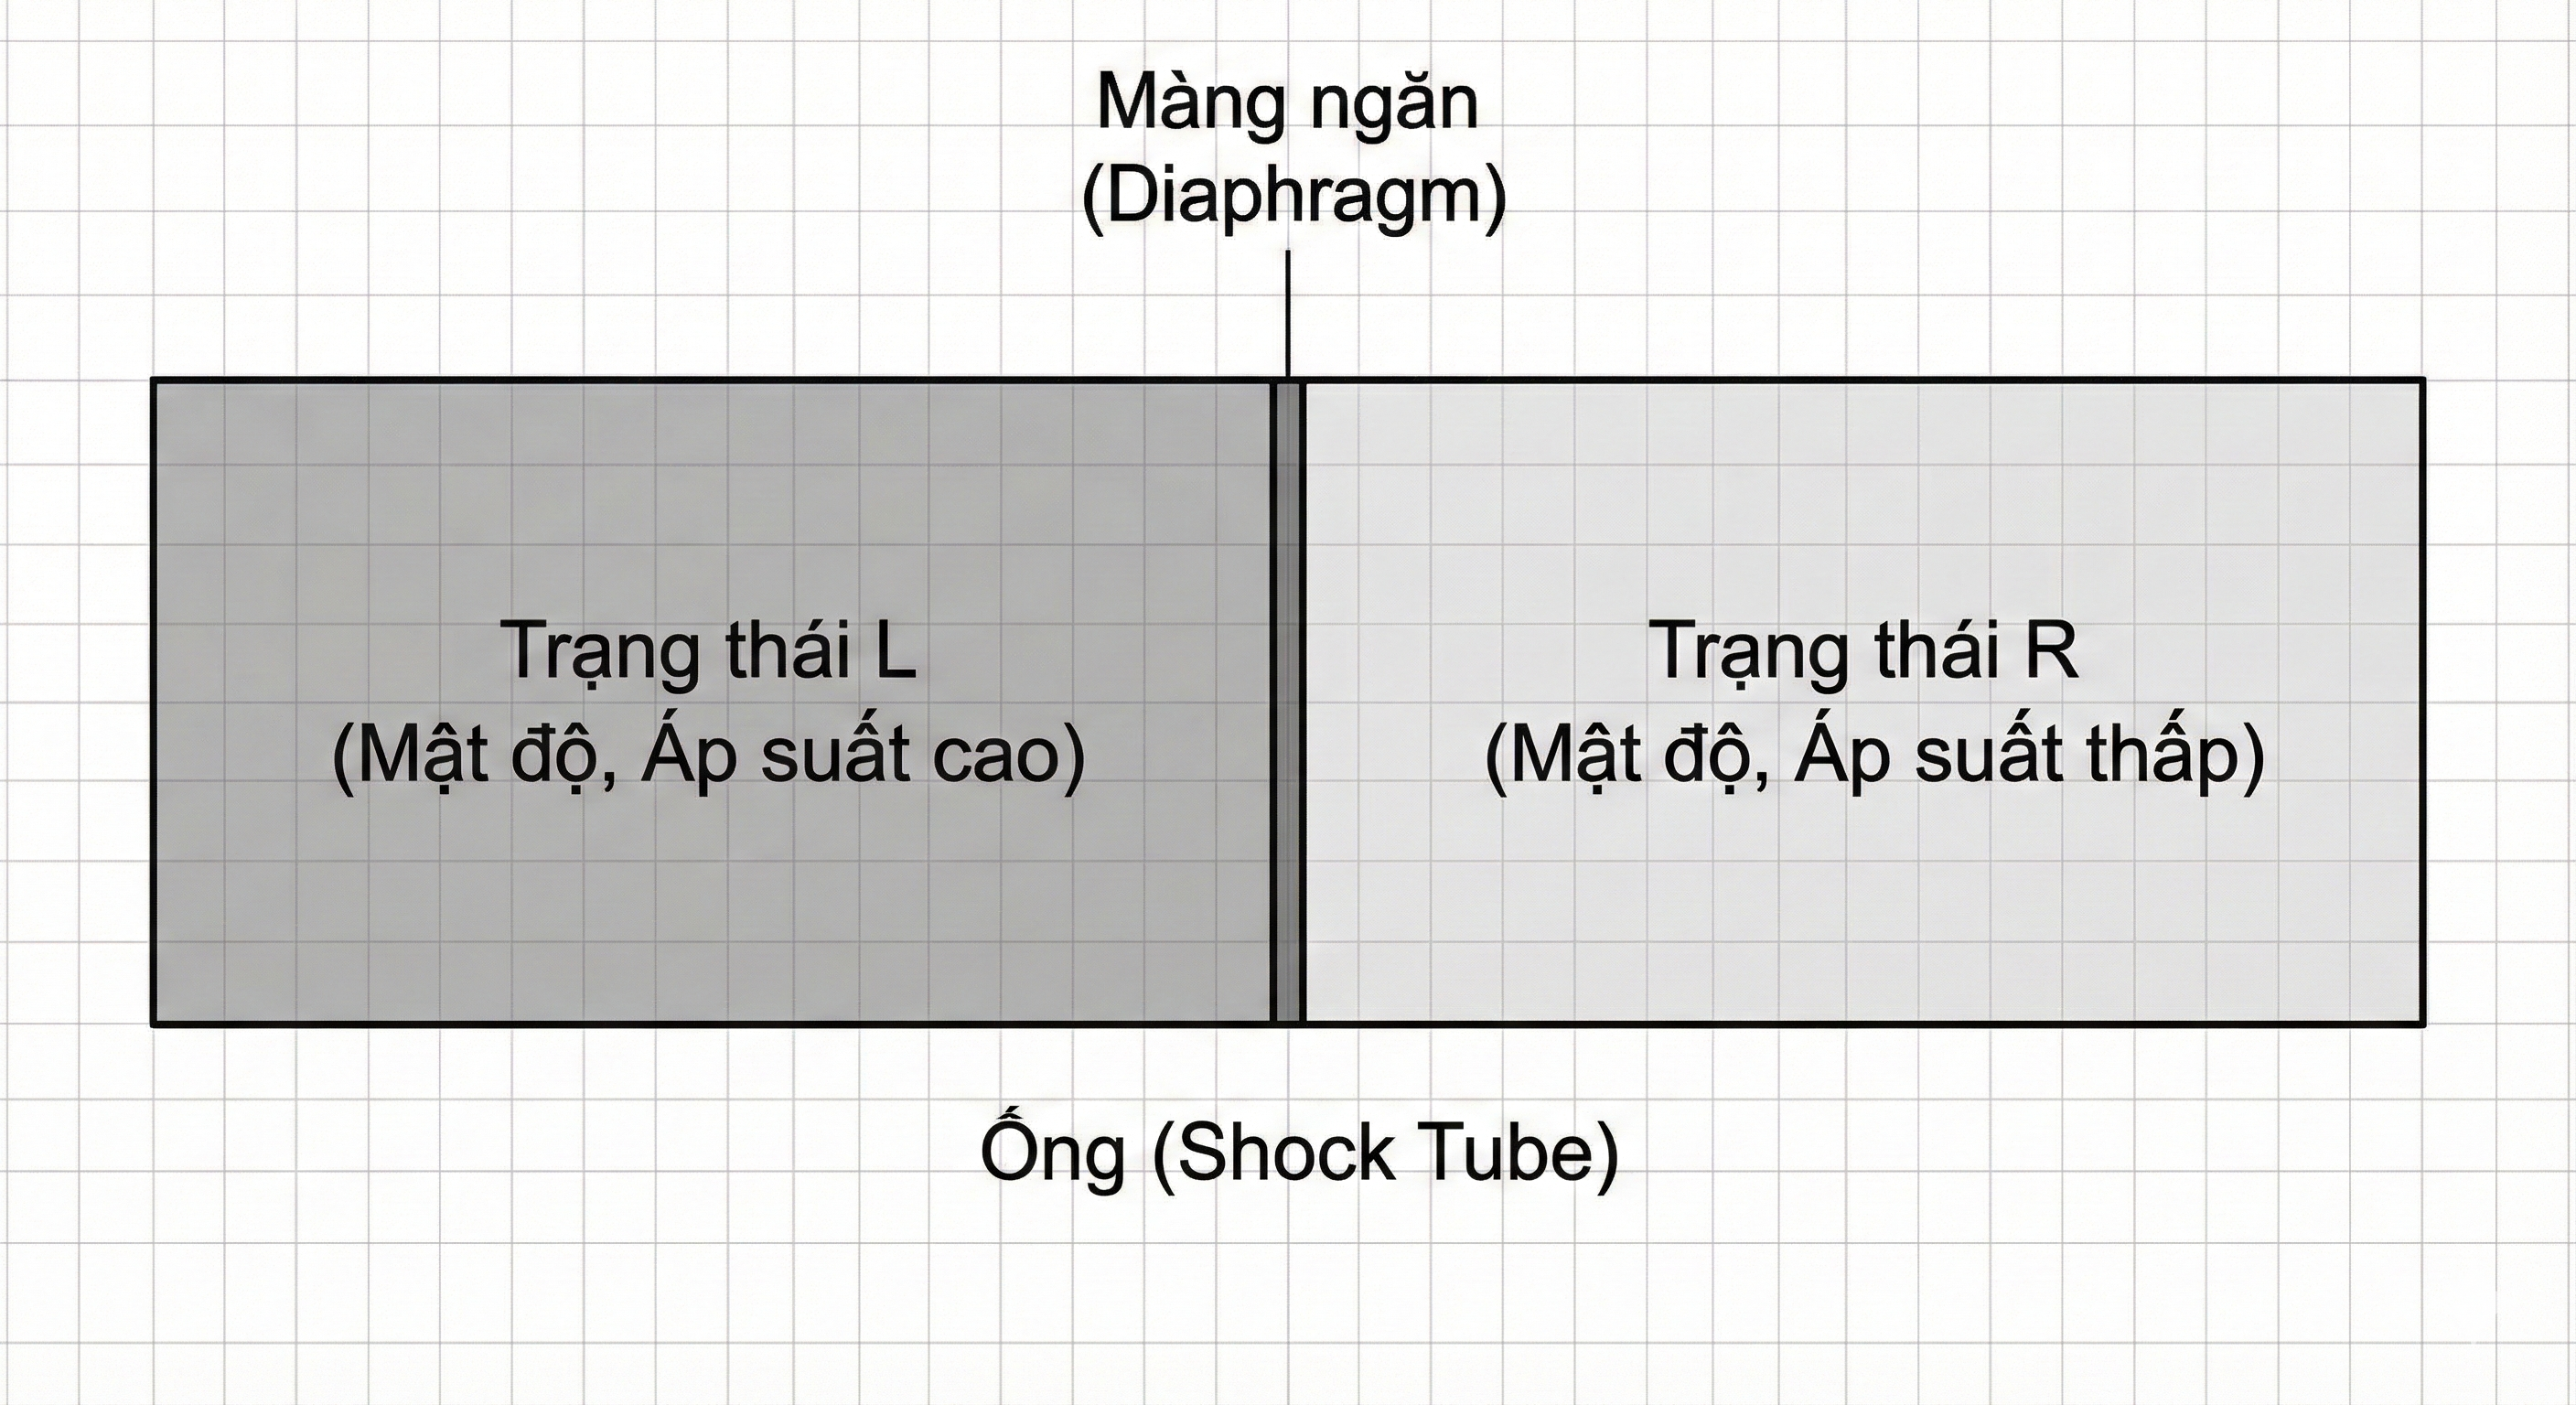
\includegraphics[width=\textwidth]{tube.png}
\end{center}
\end{column}
\end{columns}
\end{frame}

\begin{frame}{Cấu trúc nghiệm Riemann}
\begin{center}
\begin{tikzpicture}[scale=1.2]
% Axes
\draw[->] (0,0) -- (6,0) node[right] {$x$};
\draw[->] (0,0) -- (0,4) node[above] {$t$};

% Wave lines
\draw[thick, blue] (1,0.5) -- (2,3.5); % Rarefaction head
\draw[thick, blue] (2,0.5) -- (2.8,3.5); % Rarefaction tail
\draw[thick, red] (3,0.5) -- (3,3.5); % Contact
\draw[thick, green] (3.5,0.5) -- (4.5,3.5); % Shock

% Regions
\node[font=\Large] at (0.5,2) {L};
\node[font=\Large] at (2.4,2) {L*};
\node[font=\Large] at (3.2,2) {R*};
\node[font=\Large] at (5,2) {R};

% Labels
\node[blue] at (1.5,3.8) {Sóng giãn};
\node[red] at (3,3.8) {Tiếp xúc};
\node[green] at (4,3.8) {Shock};
\end{tikzpicture}
\end{center}
\end{frame}

\begin{frame}{Thuật toán nghiệm chính xác}
\textbf{Bước 1:} Thiết lập phương trình áp suất $p^*$
$$f(p) = u_L^*(p) - u_R^*(p) = 0$$

\textbf{Bước 2:} Newton-Raphson
$$p_{k+1} = p_k - \frac{f(p_k)}{f'(p_k)}$$

\textbf{Bước 3:} Tính biến trạng thái vùng sao

\textbf{Bước 4:} Xác định nghiệm tại $(x,t)$
\end{frame}

\begin{frame}{Kết quả nghiệm chính xác}
\begin{center}
\scalebox{0.9}{\begin{figure}[H]
\centering
\begin{tikzpicture}
    % Define spacing and dimensions
    \def\plotwidth{7cm}
    \def\plotheight{5.5cm}
    \def\hspace{8cm}
    \def\vspace{6.5cm}
    
    % Top row
    \node[anchor=south west, fill=white] at (0,\vspace) {
        \resizebox{\plotwidth}{\plotheight}{% This file was created by matlab2tikz.
%
%The latest updates can be retrieved from
%  http://www.mathworks.com/matlabcentral/fileexchange/22022-matlab2tikz-matlab2tikz
%where you can also make suggestions and rate matlab2tikz.
%
\definecolor{mycolor1}{rgb}{0.12941,0.12941,0.12941}%
%
\begin{tikzpicture}

\begin{axis}[%
width=3.229in,
height=2.498in,
at={(0.542in,0.392in)},
scale only axis,
xmin=0,
xmax=1,
xlabel style={font=\color{mycolor1}},
xlabel={x},
ymin=0.1,
ymax=1,
ylabel style={font=\color{mycolor1}},
ylabel={$\text{Density (}\rho\text{)}$},
axis background/.style={fill=white},
title style={font=\bfseries\color{mycolor1}},
title={Exact Density Distribution},
xmajorgrids,
ymajorgrids,
legend style={legend cell align=left, align=left}
]
\addplot [color=blue, line width=2.0pt]
  table[row sep=crcr]{%
0	1\\
0.001001001001001	1\\
0.002002002002002	1\\
0.003003003003003	1\\
0.004004004004004	1\\
0.005005005005005	1\\
0.00600600600600601	1\\
0.00700700700700701	1\\
0.00800800800800801	1\\
0.00900900900900901	1\\
0.01001001001001	1\\
0.011011011011011	1\\
0.012012012012012	1\\
0.013013013013013	1\\
0.014014014014014	1\\
0.015015015015015	1\\
0.016016016016016	1\\
0.017017017017017	1\\
0.018018018018018	1\\
0.019019019019019	1\\
0.02002002002002	1\\
0.021021021021021	1\\
0.022022022022022	1\\
0.023023023023023	1\\
0.024024024024024	1\\
0.025025025025025	1\\
0.026026026026026	1\\
0.027027027027027	1\\
0.028028028028028	1\\
0.029029029029029	1\\
0.03003003003003	1\\
0.031031031031031	1\\
0.032032032032032	1\\
0.033033033033033	1\\
0.034034034034034	1\\
0.035035035035035	1\\
0.036036036036036	1\\
0.037037037037037	1\\
0.038038038038038	1\\
0.039039039039039	1\\
0.04004004004004	1\\
0.041041041041041	1\\
0.042042042042042	1\\
0.043043043043043	1\\
0.044044044044044	1\\
0.045045045045045	1\\
0.046046046046046	1\\
0.047047047047047	1\\
0.048048048048048	1\\
0.049049049049049	1\\
0.0500500500500501	1\\
0.0510510510510511	1\\
0.0520520520520521	1\\
0.0530530530530531	1\\
0.0540540540540541	1\\
0.0550550550550551	1\\
0.0560560560560561	1\\
0.0570570570570571	1\\
0.0580580580580581	1\\
0.0590590590590591	1\\
0.0600600600600601	1\\
0.0610610610610611	1\\
0.0620620620620621	1\\
0.0630630630630631	1\\
0.0640640640640641	1\\
0.0650650650650651	1\\
0.0660660660660661	1\\
0.0670670670670671	1\\
0.0680680680680681	1\\
0.0690690690690691	1\\
0.0700700700700701	1\\
0.0710710710710711	1\\
0.0720720720720721	1\\
0.0730730730730731	1\\
0.0740740740740741	1\\
0.0750750750750751	1\\
0.0760760760760761	1\\
0.0770770770770771	1\\
0.0780780780780781	1\\
0.0790790790790791	1\\
0.0800800800800801	1\\
0.0810810810810811	1\\
0.0820820820820821	1\\
0.0830830830830831	1\\
0.0840840840840841	1\\
0.0850850850850851	1\\
0.0860860860860861	1\\
0.0870870870870871	1\\
0.0880880880880881	1\\
0.0890890890890891	1\\
0.0900900900900901	1\\
0.0910910910910911	1\\
0.0920920920920921	1\\
0.0930930930930931	1\\
0.0940940940940941	1\\
0.0950950950950951	1\\
0.0960960960960961	1\\
0.0970970970970971	1\\
0.0980980980980981	1\\
0.0990990990990991	1\\
0.1001001001001	1\\
0.101101101101101	1\\
0.102102102102102	1\\
0.103103103103103	1\\
0.104104104104104	1\\
0.105105105105105	1\\
0.106106106106106	1\\
0.107107107107107	1\\
0.108108108108108	1\\
0.109109109109109	1\\
0.11011011011011	1\\
0.111111111111111	1\\
0.112112112112112	1\\
0.113113113113113	1\\
0.114114114114114	1\\
0.115115115115115	1\\
0.116116116116116	1\\
0.117117117117117	1\\
0.118118118118118	1\\
0.119119119119119	1\\
0.12012012012012	1\\
0.121121121121121	1\\
0.122122122122122	1\\
0.123123123123123	1\\
0.124124124124124	1\\
0.125125125125125	1\\
0.126126126126126	1\\
0.127127127127127	1\\
0.128128128128128	1\\
0.129129129129129	1\\
0.13013013013013	1\\
0.131131131131131	1\\
0.132132132132132	1\\
0.133133133133133	1\\
0.134134134134134	1\\
0.135135135135135	1\\
0.136136136136136	1\\
0.137137137137137	1\\
0.138138138138138	1\\
0.139139139139139	1\\
0.14014014014014	1\\
0.141141141141141	1\\
0.142142142142142	1\\
0.143143143143143	1\\
0.144144144144144	1\\
0.145145145145145	1\\
0.146146146146146	1\\
0.147147147147147	1\\
0.148148148148148	1\\
0.149149149149149	1\\
0.15015015015015	1\\
0.151151151151151	1\\
0.152152152152152	1\\
0.153153153153153	1\\
0.154154154154154	1\\
0.155155155155155	1\\
0.156156156156156	1\\
0.157157157157157	1\\
0.158158158158158	1\\
0.159159159159159	1\\
0.16016016016016	1\\
0.161161161161161	1\\
0.162162162162162	1\\
0.163163163163163	1\\
0.164164164164164	1\\
0.165165165165165	1\\
0.166166166166166	1\\
0.167167167167167	1\\
0.168168168168168	1\\
0.169169169169169	1\\
0.17017017017017	1\\
0.171171171171171	1\\
0.172172172172172	1\\
0.173173173173173	1\\
0.174174174174174	1\\
0.175175175175175	1\\
0.176176176176176	1\\
0.177177177177177	1\\
0.178178178178178	1\\
0.179179179179179	1\\
0.18018018018018	1\\
0.181181181181181	1\\
0.182182182182182	1\\
0.183183183183183	1\\
0.184184184184184	1\\
0.185185185185185	1\\
0.186186186186186	1\\
0.187187187187187	1\\
0.188188188188188	1\\
0.189189189189189	1\\
0.19019019019019	1\\
0.191191191191191	1\\
0.192192192192192	1\\
0.193193193193193	1\\
0.194194194194194	1\\
0.195195195195195	1\\
0.196196196196196	1\\
0.197197197197197	1\\
0.198198198198198	1\\
0.199199199199199	1\\
0.2002002002002	1\\
0.201201201201201	1\\
0.202202202202202	1\\
0.203203203203203	1\\
0.204204204204204	1\\
0.205205205205205	1\\
0.206206206206206	1\\
0.207207207207207	1\\
0.208208208208208	1\\
0.209209209209209	1\\
0.21021021021021	1\\
0.211211211211211	1\\
0.212212212212212	1\\
0.213213213213213	1\\
0.214214214214214	1\\
0.215215215215215	1\\
0.216216216216216	1\\
0.217217217217217	1\\
0.218218218218218	1\\
0.219219219219219	1\\
0.22022022022022	1\\
0.221221221221221	1\\
0.222222222222222	1\\
0.223223223223223	1\\
0.224224224224224	1\\
0.225225225225225	1\\
0.226226226226226	1\\
0.227227227227227	1\\
0.228228228228228	1\\
0.229229229229229	1\\
0.23023023023023	1\\
0.231231231231231	1\\
0.232232232232232	1\\
0.233233233233233	1\\
0.234234234234234	1\\
0.235235235235235	1\\
0.236236236236236	1\\
0.237237237237237	1\\
0.238238238238238	1\\
0.239239239239239	1\\
0.24024024024024	1\\
0.241241241241241	1\\
0.242242242242242	1\\
0.243243243243243	1\\
0.244244244244244	1\\
0.245245245245245	1\\
0.246246246246246	1\\
0.247247247247247	1\\
0.248248248248248	1\\
0.249249249249249	1\\
0.25025025025025	1\\
0.251251251251251	1\\
0.252252252252252	1\\
0.253253253253253	1\\
0.254254254254254	1\\
0.255255255255255	1\\
0.256256256256256	1\\
0.257257257257257	1\\
0.258258258258258	1\\
0.259259259259259	1\\
0.26026026026026	1\\
0.261261261261261	1\\
0.262262262262262	1\\
0.263263263263263	1\\
0.264264264264264	0.996808498960078\\
0.265265265265265	0.993297458040382\\
0.266266266266266	0.989796317599393\\
0.267267267267267	0.986305056684211\\
0.268268268268268	0.982823654371522\\
0.269269269269269	0.97935208976757\\
0.27027027027027	0.975890342008143\\
0.271271271271271	0.97243839025855\\
0.272272272272272	0.968996213713598\\
0.273273273273273	0.965563791597575\\
0.274274274274274	0.962141103164227\\
0.275275275275275	0.958728127696733\\
0.276276276276276	0.955324844507693\\
0.277277277277277	0.9519312329391\\
0.278278278278278	0.948547272362322\\
0.279279279279279	0.94517294217808\\
0.28028028028028	0.941808221816428\\
0.281281281281281	0.938453090736732\\
0.282282282282282	0.935107528427646\\
0.283283283283283	0.931771514407098\\
0.284284284284284	0.928445028222263\\
0.285285285285285	0.925128049449543\\
0.286286286286286	0.921820557694549\\
0.287287287287287	0.918522532592077\\
0.288288288288288	0.915233953806091\\
0.289289289289289	0.911954801029695\\
0.29029029029029	0.908685053985118\\
0.291291291291291	0.905424692423697\\
0.292292292292292	0.902173696125843\\
0.293293293293293	0.898932044901032\\
0.294294294294294	0.895699718587779\\
0.295295295295295	0.89247669705362\\
0.296296296296296	0.889262960195086\\
0.297297297297297	0.886058487937686\\
0.298298298298298	0.882863260235888\\
0.299299299299299	0.879677257073092\\
0.3003003003003	0.876500458461617\\
0.301301301301301	0.87333284444267\\
0.302302302302302	0.870174395086335\\
0.303303303303303	0.867025090491547\\
0.304304304304304	0.86388491078607\\
0.305305305305305	0.860753836126482\\
0.306306306306306	0.857631846698146\\
0.307307307307307	0.854518922715196\\
0.308308308308308	0.851415044420512\\
0.309309309309309	0.848320192085701\\
0.31031031031031	0.845234346011077\\
0.311311311311311	0.842157486525636\\
0.312312312312312	0.839089593987038\\
0.313313313313313	0.83603064878159\\
0.314314314314314	0.832980631324216\\
0.315315315315315	0.829939522058443\\
0.316316316316316	0.82690730145638\\
0.317317317317317	0.823883950018692\\
0.318318318318318	0.820869448274584\\
0.319319319319319	0.817863776781779\\
0.32032032032032	0.814866916126497\\
0.321321321321321	0.81187884692343\\
0.322322322322322	0.808899549815731\\
0.323323323323323	0.805929005474981\\
0.324324324324324	0.802967194601177\\
0.325325325325325	0.80001409792271\\
0.326326326326326	0.797069696196337\\
0.327327327327327	0.794133970207167\\
0.328328328328328	0.791206900768644\\
0.329329329329329	0.788288468722513\\
0.33033033033033	0.785378654938809\\
0.331331331331331	0.782477440315837\\
0.332332332332332	0.779584805780143\\
0.333333333333333	0.7767007322865\\
0.334334334334334	0.773825200817887\\
0.335335335335335	0.770958192385463\\
0.336336336336336	0.768099688028551\\
0.337337337337337	0.765249668814614\\
0.338338338338338	0.762408115839236\\
0.339339339339339	0.759575010226101\\
0.34034034034034	0.756750333126972\\
0.341341341341341	0.753934065721667\\
0.342342342342342	0.751126189218046\\
0.343343343343343	0.74832668485198\\
0.344344344344344	0.745535533887337\\
0.345345345345345	0.742752717615957\\
0.346346346346346	0.739978217357638\\
0.347347347347347	0.737212014460107\\
0.348348348348348	0.734454090299001\\
0.349349349349349	0.731704426277851\\
0.35035035035035	0.728963003828056\\
0.351351351351351	0.726229804408862\\
0.352352352352352	0.723504809507348\\
0.353353353353353	0.720788000638393\\
0.354354354354354	0.718079359344668\\
0.355355355355355	0.715378867196605\\
0.356356356356356	0.712686505792382\\
0.357357357357357	0.710002256757903\\
0.358358358358358	0.707326101746769\\
0.359359359359359	0.704658022440265\\
0.36036036036036	0.701998000547337\\
0.361361361361361	0.699346017804573\\
0.362362362362362	0.696702055976176\\
0.363363363363363	0.694066096853946\\
0.364364364364364	0.691438122257266\\
0.365365365365365	0.68881811403307\\
0.366366366366366	0.686206054055828\\
0.367367367367367	0.683601924227527\\
0.368368368368368	0.681005706477644\\
0.369369369369369	0.678417382763132\\
0.37037037037037	0.675836935068391\\
0.371371371371371	0.673264345405257\\
0.372372372372372	0.670699595812972\\
0.373373373373373	0.668142668358169\\
0.374374374374374	0.665593545134849\\
0.375375375375375	0.663052208264357\\
0.376376376376376	0.660518639895369\\
0.377377377377377	0.657992822203864\\
0.378378378378378	0.655474737393104\\
0.379379379379379	0.652964367693619\\
0.38038038038038	0.650461695363176\\
0.381381381381381	0.647966702686767\\
0.382382382382382	0.645479371976586\\
0.383383383383383	0.642999685572005\\
0.384384384384384	0.640527625839553\\
0.385385385385385	0.638063175172903\\
0.386386386386386	0.635606315992839\\
0.387387387387387	0.633157030747246\\
0.388388388388388	0.630715301911081\\
0.389389389389389	0.62828111198636\\
0.39039039039039	0.625854443502127\\
0.391391391391391	0.623435279014443\\
0.392392392392392	0.62102360110636\\
0.393393393393393	0.618619392387899\\
0.394394394394394	0.616222635496034\\
0.395395395395395	0.613833313094666\\
0.396396396396396	0.611451407874604\\
0.397397397397397	0.609076902553548\\
0.398398398398398	0.606709779876059\\
0.399399399399399	0.604350022613548\\
0.4004004004004	0.601997613564249\\
0.401401401401401	0.599652535553199\\
0.402402402402402	0.59731477143222\\
0.403403403403403	0.594984304079894\\
0.404404404404404	0.592661116401545\\
0.405405405405405	0.590345191329216\\
0.406406406406406	0.588036511821652\\
0.407407407407407	0.585735060864273\\
0.408408408408408	0.583440821469158\\
0.409409409409409	0.581153776675024\\
0.41041041041041	0.578873909547202\\
0.411411411411411	0.576601203177618\\
0.412412412412412	0.574335640684771\\
0.413413413413413	0.572077205213716\\
0.414414414414414	0.569825879936036\\
0.415415415415415	0.567581648049829\\
0.416416416416416	0.56534449277968\\
0.417417417417417	0.563114397376647\\
0.418418418418418	0.560891345118232\\
0.419419419419419	0.55867531930837\\
0.42042042042042	0.556466303277396\\
0.421421421421421	0.554264280382037\\
0.422422422422422	0.552069234005383\\
0.423423423423423	0.549881147556865\\
0.424424424424424	0.547700004472242\\
0.425425425425425	0.545525788213571\\
0.426426426426426	0.543358482269192\\
0.427427427427427	0.541198070153706\\
0.428428428428428	0.539044535407954\\
0.429429429429429	0.536897861598993\\
0.43043043043043	0.534758032320079\\
0.431431431431431	0.532625031190645\\
0.432432432432432	0.530498841856281\\
0.433433433433433	0.52837944798871\\
0.434434434434434	0.526266833285771\\
0.435435435435435	0.524160981471394\\
0.436436436436436	0.522061876295583\\
0.437437437437437	0.519969501534392\\
0.438438438438438	0.517883840989908\\
0.439439439439439	0.515804878490226\\
0.44044044044044	0.513732597889428\\
0.441441441441441	0.511666983067567\\
0.442442442442442	0.50960801793064\\
0.443443443443443	0.507555686410575\\
0.444444444444444	0.505509972465197\\
0.445445445445445	0.503470860078223\\
0.446446446446446	0.501438333259228\\
0.447447447447447	0.499412376043634\\
0.448448448448448	0.49739297249268\\
0.449449449449449	0.495380106693409\\
0.45045045045045	0.49337376275864\\
0.451451451451451	0.491373924826956\\
0.452452452452452	0.489380577062674\\
0.453453453453453	0.487393703655828\\
0.454454454454454	0.485413288822151\\
0.455455455455455	0.48343931680305\\
0.456456456456456	0.481471771865583\\
0.457457457457457	0.479510638302447\\
0.458458458458458	0.477555900431948\\
0.459459459459459	0.475607542597983\\
0.46046046046046	0.473665549170023\\
0.461461461461461	0.471729904543085\\
0.462462462462462	0.469800593137719\\
0.463463463463463	0.467877599399979\\
0.464464464464464	0.46596090780141\\
0.465465465465465	0.464050502839019\\
0.466466466466466	0.462146369035263\\
0.467467467467467	0.460248490938019\\
0.468468468468468	0.458356853120571\\
0.469469469469469	0.456471440181583\\
0.47047047047047	0.454592236745083\\
0.471471471471471	0.452719227460437\\
0.472472472472472	0.450852397002335\\
0.473473473473473	0.448991730070763\\
0.474474474474474	0.447137211390985\\
0.475475475475475	0.445288825713525\\
0.476476476476476	0.443446557814139\\
0.477477477477477	0.441610392493802\\
0.478478478478478	0.439780314578683\\
0.479479479479479	0.437956308920124\\
0.48048048048048	0.436138360394619\\
0.481481481481481	0.434326453903796\\
0.482482482482482	0.432520574374392\\
0.483483483483483	0.430720706758233\\
0.484484484484485	0.428926836032218\\
0.485485485485485	0.427138947198293\\
0.486486486486487	0.426319428178495\\
0.487487487487487	0.426319428178495\\
0.488488488488488	0.426319428178495\\
0.48948948948949	0.426319428178495\\
0.49049049049049	0.426319428178495\\
0.491491491491492	0.426319428178495\\
0.492492492492492	0.426319428178495\\
0.493493493493493	0.426319428178495\\
0.494494494494495	0.426319428178495\\
0.495495495495495	0.426319428178495\\
0.496496496496497	0.426319428178495\\
0.497497497497497	0.426319428178495\\
0.498498498498498	0.426319428178495\\
0.4994994994995	0.426319428178495\\
0.500500500500501	0.426319428178495\\
0.501501501501502	0.426319428178495\\
0.502502502502503	0.426319428178495\\
0.503503503503503	0.426319428178495\\
0.504504504504504	0.426319428178495\\
0.505505505505506	0.426319428178495\\
0.506506506506507	0.426319428178495\\
0.507507507507508	0.426319428178495\\
0.508508508508508	0.426319428178495\\
0.509509509509509	0.426319428178495\\
0.510510510510511	0.426319428178495\\
0.511511511511512	0.426319428178495\\
0.512512512512513	0.426319428178495\\
0.513513513513513	0.426319428178495\\
0.514514514514514	0.426319428178495\\
0.515515515515516	0.426319428178495\\
0.516516516516517	0.426319428178495\\
0.517517517517518	0.426319428178495\\
0.518518518518518	0.426319428178495\\
0.519519519519519	0.426319428178495\\
0.520520520520521	0.426319428178495\\
0.521521521521522	0.426319428178495\\
0.522522522522523	0.426319428178495\\
0.523523523523523	0.426319428178495\\
0.524524524524524	0.426319428178495\\
0.525525525525526	0.426319428178495\\
0.526526526526527	0.426319428178495\\
0.527527527527528	0.426319428178495\\
0.528528528528528	0.426319428178495\\
0.529529529529529	0.426319428178495\\
0.530530530530531	0.426319428178495\\
0.531531531531532	0.426319428178495\\
0.532532532532533	0.426319428178495\\
0.533533533533533	0.426319428178495\\
0.534534534534535	0.426319428178495\\
0.535535535535536	0.426319428178495\\
0.536536536536537	0.426319428178495\\
0.537537537537538	0.426319428178495\\
0.538538538538539	0.426319428178495\\
0.53953953953954	0.426319428178495\\
0.540540540540541	0.426319428178495\\
0.541541541541542	0.426319428178495\\
0.542542542542543	0.426319428178495\\
0.543543543543544	0.426319428178495\\
0.544544544544545	0.426319428178495\\
0.545545545545546	0.426319428178495\\
0.546546546546547	0.426319428178495\\
0.547547547547548	0.426319428178495\\
0.548548548548549	0.426319428178495\\
0.54954954954955	0.426319428178495\\
0.550550550550551	0.426319428178495\\
0.551551551551552	0.426319428178495\\
0.552552552552553	0.426319428178495\\
0.553553553553554	0.426319428178495\\
0.554554554554555	0.426319428178495\\
0.555555555555556	0.426319428178495\\
0.556556556556557	0.426319428178495\\
0.557557557557558	0.426319428178495\\
0.558558558558559	0.426319428178495\\
0.55955955955956	0.426319428178495\\
0.560560560560561	0.426319428178495\\
0.561561561561562	0.426319428178495\\
0.562562562562563	0.426319428178495\\
0.563563563563564	0.426319428178495\\
0.564564564564565	0.426319428178495\\
0.565565565565566	0.426319428178495\\
0.566566566566567	0.426319428178495\\
0.567567567567568	0.426319428178495\\
0.568568568568569	0.426319428178495\\
0.56956956956957	0.426319428178495\\
0.570570570570571	0.426319428178495\\
0.571571571571572	0.426319428178495\\
0.572572572572573	0.426319428178495\\
0.573573573573574	0.426319428178495\\
0.574574574574575	0.426319428178495\\
0.575575575575576	0.426319428178495\\
0.576576576576577	0.426319428178495\\
0.577577577577578	0.426319428178495\\
0.578578578578579	0.426319428178495\\
0.57957957957958	0.426319428178495\\
0.580580580580581	0.426319428178495\\
0.581581581581582	0.426319428178495\\
0.582582582582583	0.426319428178495\\
0.583583583583584	0.426319428178495\\
0.584584584584585	0.426319428178495\\
0.585585585585586	0.426319428178495\\
0.586586586586587	0.426319428178495\\
0.587587587587588	0.426319428178495\\
0.588588588588589	0.426319428178495\\
0.58958958958959	0.426319428178495\\
0.590590590590591	0.426319428178495\\
0.591591591591592	0.426319428178495\\
0.592592592592593	0.426319428178495\\
0.593593593593594	0.426319428178495\\
0.594594594594595	0.426319428178495\\
0.595595595595596	0.426319428178495\\
0.596596596596597	0.426319428178495\\
0.597597597597598	0.426319428178495\\
0.598598598598599	0.426319428178495\\
0.5995995995996	0.426319428178495\\
0.600600600600601	0.426319428178495\\
0.601601601601602	0.426319428178495\\
0.602602602602603	0.426319428178495\\
0.603603603603604	0.426319428178495\\
0.604604604604605	0.426319428178495\\
0.605605605605606	0.426319428178495\\
0.606606606606607	0.426319428178495\\
0.607607607607608	0.426319428178495\\
0.608608608608609	0.426319428178495\\
0.60960960960961	0.426319428178495\\
0.610610610610611	0.426319428178495\\
0.611611611611612	0.426319428178495\\
0.612612612612613	0.426319428178495\\
0.613613613613614	0.426319428178495\\
0.614614614614615	0.426319428178495\\
0.615615615615616	0.426319428178495\\
0.616616616616617	0.426319428178495\\
0.617617617617618	0.426319428178495\\
0.618618618618619	0.426319428178495\\
0.61961961961962	0.426319428178495\\
0.620620620620621	0.426319428178495\\
0.621621621621622	0.426319428178495\\
0.622622622622623	0.426319428178495\\
0.623623623623624	0.426319428178495\\
0.624624624624625	0.426319428178495\\
0.625625625625626	0.426319428178495\\
0.626626626626627	0.426319428178495\\
0.627627627627628	0.426319428178495\\
0.628628628628629	0.426319428178495\\
0.62962962962963	0.426319428178495\\
0.630630630630631	0.426319428178495\\
0.631631631631632	0.426319428178495\\
0.632632632632633	0.426319428178495\\
0.633633633633634	0.426319428178495\\
0.634634634634635	0.426319428178495\\
0.635635635635636	0.426319428178495\\
0.636636636636637	0.426319428178495\\
0.637637637637638	0.426319428178495\\
0.638638638638639	0.426319428178495\\
0.63963963963964	0.426319428178495\\
0.640640640640641	0.426319428178495\\
0.641641641641642	0.426319428178495\\
0.642642642642643	0.426319428178495\\
0.643643643643644	0.426319428178495\\
0.644644644644645	0.426319428178495\\
0.645645645645646	0.426319428178495\\
0.646646646646647	0.426319428178495\\
0.647647647647648	0.426319428178495\\
0.648648648648649	0.426319428178495\\
0.64964964964965	0.426319428178495\\
0.650650650650651	0.426319428178495\\
0.651651651651652	0.426319428178495\\
0.652652652652653	0.426319428178495\\
0.653653653653654	0.426319428178495\\
0.654654654654655	0.426319428178495\\
0.655655655655656	0.426319428178495\\
0.656656656656657	0.426319428178495\\
0.657657657657658	0.426319428178495\\
0.658658658658659	0.426319428178495\\
0.65965965965966	0.426319428178495\\
0.660660660660661	0.426319428178495\\
0.661661661661662	0.426319428178495\\
0.662662662662663	0.426319428178495\\
0.663663663663664	0.426319428178495\\
0.664664664664665	0.426319428178495\\
0.665665665665666	0.426319428178495\\
0.666666666666667	0.426319428178495\\
0.667667667667668	0.426319428178495\\
0.668668668668669	0.426319428178495\\
0.66966966966967	0.426319428178495\\
0.670670670670671	0.426319428178495\\
0.671671671671672	0.426319428178495\\
0.672672672672673	0.426319428178495\\
0.673673673673674	0.426319428178495\\
0.674674674674675	0.426319428178495\\
0.675675675675676	0.426319428178495\\
0.676676676676677	0.426319428178495\\
0.677677677677678	0.426319428178495\\
0.678678678678679	0.426319428178495\\
0.67967967967968	0.426319428178495\\
0.680680680680681	0.426319428178495\\
0.681681681681682	0.426319428178495\\
0.682682682682683	0.426319428178495\\
0.683683683683684	0.426319428178495\\
0.684684684684685	0.426319428178495\\
0.685685685685686	0.265573711705307\\
0.686686686686687	0.265573711705307\\
0.687687687687688	0.265573711705307\\
0.688688688688689	0.265573711705307\\
0.68968968968969	0.265573711705307\\
0.690690690690691	0.265573711705307\\
0.691691691691692	0.265573711705307\\
0.692692692692693	0.265573711705307\\
0.693693693693694	0.265573711705307\\
0.694694694694695	0.265573711705307\\
0.695695695695696	0.265573711705307\\
0.696696696696697	0.265573711705307\\
0.697697697697698	0.265573711705307\\
0.698698698698699	0.265573711705307\\
0.6996996996997	0.265573711705307\\
0.700700700700701	0.265573711705307\\
0.701701701701702	0.265573711705307\\
0.702702702702703	0.265573711705307\\
0.703703703703704	0.265573711705307\\
0.704704704704705	0.265573711705307\\
0.705705705705706	0.265573711705307\\
0.706706706706707	0.265573711705307\\
0.707707707707708	0.265573711705307\\
0.708708708708709	0.265573711705307\\
0.70970970970971	0.265573711705307\\
0.710710710710711	0.265573711705307\\
0.711711711711712	0.265573711705307\\
0.712712712712713	0.265573711705307\\
0.713713713713714	0.265573711705307\\
0.714714714714715	0.265573711705307\\
0.715715715715716	0.265573711705307\\
0.716716716716717	0.265573711705307\\
0.717717717717718	0.265573711705307\\
0.718718718718719	0.265573711705307\\
0.71971971971972	0.265573711705307\\
0.720720720720721	0.265573711705307\\
0.721721721721722	0.265573711705307\\
0.722722722722723	0.265573711705307\\
0.723723723723724	0.265573711705307\\
0.724724724724725	0.265573711705307\\
0.725725725725726	0.265573711705307\\
0.726726726726727	0.265573711705307\\
0.727727727727728	0.265573711705307\\
0.728728728728729	0.265573711705307\\
0.72972972972973	0.265573711705307\\
0.730730730730731	0.265573711705307\\
0.731731731731732	0.265573711705307\\
0.732732732732733	0.265573711705307\\
0.733733733733734	0.265573711705307\\
0.734734734734735	0.265573711705307\\
0.735735735735736	0.265573711705307\\
0.736736736736737	0.265573711705307\\
0.737737737737738	0.265573711705307\\
0.738738738738739	0.265573711705307\\
0.73973973973974	0.265573711705307\\
0.740740740740741	0.265573711705307\\
0.741741741741742	0.265573711705307\\
0.742742742742743	0.265573711705307\\
0.743743743743744	0.265573711705307\\
0.744744744744745	0.265573711705307\\
0.745745745745746	0.265573711705307\\
0.746746746746747	0.265573711705307\\
0.747747747747748	0.265573711705307\\
0.748748748748749	0.265573711705307\\
0.74974974974975	0.265573711705307\\
0.750750750750751	0.265573711705307\\
0.751751751751752	0.265573711705307\\
0.752752752752753	0.265573711705307\\
0.753753753753754	0.265573711705307\\
0.754754754754755	0.265573711705307\\
0.755755755755756	0.265573711705307\\
0.756756756756757	0.265573711705307\\
0.757757757757758	0.265573711705307\\
0.758758758758759	0.265573711705307\\
0.75975975975976	0.265573711705307\\
0.760760760760761	0.265573711705307\\
0.761761761761762	0.265573711705307\\
0.762762762762763	0.265573711705307\\
0.763763763763764	0.265573711705307\\
0.764764764764765	0.265573711705307\\
0.765765765765766	0.265573711705307\\
0.766766766766767	0.265573711705307\\
0.767767767767768	0.265573711705307\\
0.768768768768769	0.265573711705307\\
0.76976976976977	0.265573711705307\\
0.770770770770771	0.265573711705307\\
0.771771771771772	0.265573711705307\\
0.772772772772773	0.265573711705307\\
0.773773773773774	0.265573711705307\\
0.774774774774775	0.265573711705307\\
0.775775775775776	0.265573711705307\\
0.776776776776777	0.265573711705307\\
0.777777777777778	0.265573711705307\\
0.778778778778779	0.265573711705307\\
0.77977977977978	0.265573711705307\\
0.780780780780781	0.265573711705307\\
0.781781781781782	0.265573711705307\\
0.782782782782783	0.265573711705307\\
0.783783783783784	0.265573711705307\\
0.784784784784785	0.265573711705307\\
0.785785785785786	0.265573711705307\\
0.786786786786787	0.265573711705307\\
0.787787787787788	0.265573711705307\\
0.788788788788789	0.265573711705307\\
0.78978978978979	0.265573711705307\\
0.790790790790791	0.265573711705307\\
0.791791791791792	0.265573711705307\\
0.792792792792793	0.265573711705307\\
0.793793793793794	0.265573711705307\\
0.794794794794795	0.265573711705307\\
0.795795795795796	0.265573711705307\\
0.796796796796797	0.265573711705307\\
0.797797797797798	0.265573711705307\\
0.798798798798799	0.265573711705307\\
0.7997997997998	0.265573711705307\\
0.800800800800801	0.265573711705307\\
0.801801801801802	0.265573711705307\\
0.802802802802803	0.265573711705307\\
0.803803803803804	0.265573711705307\\
0.804804804804805	0.265573711705307\\
0.805805805805806	0.265573711705307\\
0.806806806806807	0.265573711705307\\
0.807807807807808	0.265573711705307\\
0.808808808808809	0.265573711705307\\
0.80980980980981	0.265573711705307\\
0.810810810810811	0.265573711705307\\
0.811811811811812	0.265573711705307\\
0.812812812812813	0.265573711705307\\
0.813813813813814	0.265573711705307\\
0.814814814814815	0.265573711705307\\
0.815815815815816	0.265573711705307\\
0.816816816816817	0.265573711705307\\
0.817817817817818	0.265573711705307\\
0.818818818818819	0.265573711705307\\
0.81981981981982	0.265573711705307\\
0.820820820820821	0.265573711705307\\
0.821821821821822	0.265573711705307\\
0.822822822822823	0.265573711705307\\
0.823823823823824	0.265573711705307\\
0.824824824824825	0.265573711705307\\
0.825825825825826	0.265573711705307\\
0.826826826826827	0.265573711705307\\
0.827827827827828	0.265573711705307\\
0.828828828828829	0.265573711705307\\
0.82982982982983	0.265573711705307\\
0.830830830830831	0.265573711705307\\
0.831831831831832	0.265573711705307\\
0.832832832832833	0.265573711705307\\
0.833833833833834	0.265573711705307\\
0.834834834834835	0.265573711705307\\
0.835835835835836	0.265573711705307\\
0.836836836836837	0.265573711705307\\
0.837837837837838	0.265573711705307\\
0.838838838838839	0.265573711705307\\
0.83983983983984	0.265573711705307\\
0.840840840840841	0.265573711705307\\
0.841841841841842	0.265573711705307\\
0.842842842842843	0.265573711705307\\
0.843843843843844	0.265573711705307\\
0.844844844844845	0.265573711705307\\
0.845845845845846	0.265573711705307\\
0.846846846846847	0.265573711705307\\
0.847847847847848	0.265573711705307\\
0.848848848848849	0.265573711705307\\
0.84984984984985	0.265573711705307\\
0.850850850850851	0.125\\
0.851851851851852	0.125\\
0.852852852852853	0.125\\
0.853853853853854	0.125\\
0.854854854854855	0.125\\
0.855855855855856	0.125\\
0.856856856856857	0.125\\
0.857857857857858	0.125\\
0.858858858858859	0.125\\
0.85985985985986	0.125\\
0.860860860860861	0.125\\
0.861861861861862	0.125\\
0.862862862862863	0.125\\
0.863863863863864	0.125\\
0.864864864864865	0.125\\
0.865865865865866	0.125\\
0.866866866866867	0.125\\
0.867867867867868	0.125\\
0.868868868868869	0.125\\
0.86986986986987	0.125\\
0.870870870870871	0.125\\
0.871871871871872	0.125\\
0.872872872872873	0.125\\
0.873873873873874	0.125\\
0.874874874874875	0.125\\
0.875875875875876	0.125\\
0.876876876876877	0.125\\
0.877877877877878	0.125\\
0.878878878878879	0.125\\
0.87987987987988	0.125\\
0.880880880880881	0.125\\
0.881881881881882	0.125\\
0.882882882882883	0.125\\
0.883883883883884	0.125\\
0.884884884884885	0.125\\
0.885885885885886	0.125\\
0.886886886886887	0.125\\
0.887887887887888	0.125\\
0.888888888888889	0.125\\
0.88988988988989	0.125\\
0.890890890890891	0.125\\
0.891891891891892	0.125\\
0.892892892892893	0.125\\
0.893893893893894	0.125\\
0.894894894894895	0.125\\
0.895895895895896	0.125\\
0.896896896896897	0.125\\
0.897897897897898	0.125\\
0.898898898898899	0.125\\
0.8998998998999	0.125\\
0.900900900900901	0.125\\
0.901901901901902	0.125\\
0.902902902902903	0.125\\
0.903903903903904	0.125\\
0.904904904904905	0.125\\
0.905905905905906	0.125\\
0.906906906906907	0.125\\
0.907907907907908	0.125\\
0.908908908908909	0.125\\
0.90990990990991	0.125\\
0.910910910910911	0.125\\
0.911911911911912	0.125\\
0.912912912912913	0.125\\
0.913913913913914	0.125\\
0.914914914914915	0.125\\
0.915915915915916	0.125\\
0.916916916916917	0.125\\
0.917917917917918	0.125\\
0.918918918918919	0.125\\
0.91991991991992	0.125\\
0.920920920920921	0.125\\
0.921921921921922	0.125\\
0.922922922922923	0.125\\
0.923923923923924	0.125\\
0.924924924924925	0.125\\
0.925925925925926	0.125\\
0.926926926926927	0.125\\
0.927927927927928	0.125\\
0.928928928928929	0.125\\
0.92992992992993	0.125\\
0.930930930930931	0.125\\
0.931931931931932	0.125\\
0.932932932932933	0.125\\
0.933933933933934	0.125\\
0.934934934934935	0.125\\
0.935935935935936	0.125\\
0.936936936936937	0.125\\
0.937937937937938	0.125\\
0.938938938938939	0.125\\
0.93993993993994	0.125\\
0.940940940940941	0.125\\
0.941941941941942	0.125\\
0.942942942942943	0.125\\
0.943943943943944	0.125\\
0.944944944944945	0.125\\
0.945945945945946	0.125\\
0.946946946946947	0.125\\
0.947947947947948	0.125\\
0.948948948948949	0.125\\
0.94994994994995	0.125\\
0.950950950950951	0.125\\
0.951951951951952	0.125\\
0.952952952952953	0.125\\
0.953953953953954	0.125\\
0.954954954954955	0.125\\
0.955955955955956	0.125\\
0.956956956956957	0.125\\
0.957957957957958	0.125\\
0.958958958958959	0.125\\
0.95995995995996	0.125\\
0.960960960960961	0.125\\
0.961961961961962	0.125\\
0.962962962962963	0.125\\
0.963963963963964	0.125\\
0.964964964964965	0.125\\
0.965965965965966	0.125\\
0.966966966966967	0.125\\
0.967967967967968	0.125\\
0.968968968968969	0.125\\
0.96996996996997	0.125\\
0.970970970970971	0.125\\
0.971971971971972	0.125\\
0.972972972972973	0.125\\
0.973973973973974	0.125\\
0.974974974974975	0.125\\
0.975975975975976	0.125\\
0.976976976976977	0.125\\
0.977977977977978	0.125\\
0.978978978978979	0.125\\
0.97997997997998	0.125\\
0.980980980980981	0.125\\
0.981981981981982	0.125\\
0.982982982982983	0.125\\
0.983983983983984	0.125\\
0.984984984984985	0.125\\
0.985985985985986	0.125\\
0.986986986986987	0.125\\
0.987987987987988	0.125\\
0.988988988988989	0.125\\
0.98998998998999	0.125\\
0.990990990990991	0.125\\
0.991991991991992	0.125\\
0.992992992992993	0.125\\
0.993993993993994	0.125\\
0.994994994994995	0.125\\
0.995995995995996	0.125\\
0.996996996996997	0.125\\
0.997997997997998	0.125\\
0.998998998998999	0.125\\
1	0.125\\
};
\addlegendentry{Exact Solution}

\end{axis}
\end{tikzpicture}%}
    };
    
    \node[anchor=south west, fill=white] at (\hspace,\vspace) {
        \resizebox{\plotwidth}{\plotheight}{% This file was created by matlab2tikz.
%
%The latest updates can be retrieved from
%  http://www.mathworks.com/matlabcentral/fileexchange/22022-matlab2tikz-matlab2tikz
%where you can also make suggestions and rate matlab2tikz.
%
\definecolor{mycolor1}{rgb}{0.12941,0.12941,0.12941}%
%
\begin{tikzpicture}

\begin{axis}[%
width=3.229in,
height=2.498in,
at={(0.542in,0.392in)},
scale only axis,
xmin=0,
xmax=1,
xlabel style={font=\color{mycolor1}},
xlabel={x},
ymin=0,
ymax=1,
ylabel style={font=\color{mycolor1}},
ylabel={Velocity (u)},
axis background/.style={fill=white},
title style={font=\bfseries\color{mycolor1}},
title={Exact Velocity Distribution},
xmajorgrids,
ymajorgrids,
legend style={legend cell align=left, align=left}
]
\addplot [color=red, line width=2.0pt]
  table[row sep=crcr]{%
0	0\\
0.001001001001001	0\\
0.002002002002002	0\\
0.003003003003003	0\\
0.004004004004004	0\\
0.005005005005005	0\\
0.00600600600600601	0\\
0.00700700700700701	0\\
0.00800800800800801	0\\
0.00900900900900901	0\\
0.01001001001001	0\\
0.011011011011011	0\\
0.012012012012012	0\\
0.013013013013013	0\\
0.014014014014014	0\\
0.015015015015015	0\\
0.016016016016016	0\\
0.017017017017017	0\\
0.018018018018018	0\\
0.019019019019019	0\\
0.02002002002002	0\\
0.021021021021021	0\\
0.022022022022022	0\\
0.023023023023023	0\\
0.024024024024024	0\\
0.025025025025025	0\\
0.026026026026026	0\\
0.027027027027027	0\\
0.028028028028028	0\\
0.029029029029029	0\\
0.03003003003003	0\\
0.031031031031031	0\\
0.032032032032032	0\\
0.033033033033033	0\\
0.034034034034034	0\\
0.035035035035035	0\\
0.036036036036036	0\\
0.037037037037037	0\\
0.038038038038038	0\\
0.039039039039039	0\\
0.04004004004004	0\\
0.041041041041041	0\\
0.042042042042042	0\\
0.043043043043043	0\\
0.044044044044044	0\\
0.045045045045045	0\\
0.046046046046046	0\\
0.047047047047047	0\\
0.048048048048048	0\\
0.049049049049049	0\\
0.0500500500500501	0\\
0.0510510510510511	0\\
0.0520520520520521	0\\
0.0530530530530531	0\\
0.0540540540540541	0\\
0.0550550550550551	0\\
0.0560560560560561	0\\
0.0570570570570571	0\\
0.0580580580580581	0\\
0.0590590590590591	0\\
0.0600600600600601	0\\
0.0610610610610611	0\\
0.0620620620620621	0\\
0.0630630630630631	0\\
0.0640640640640641	0\\
0.0650650650650651	0\\
0.0660660660660661	0\\
0.0670670670670671	0\\
0.0680680680680681	0\\
0.0690690690690691	0\\
0.0700700700700701	0\\
0.0710710710710711	0\\
0.0720720720720721	0\\
0.0730730730730731	0\\
0.0740740740740741	0\\
0.0750750750750751	0\\
0.0760760760760761	0\\
0.0770770770770771	0\\
0.0780780780780781	0\\
0.0790790790790791	0\\
0.0800800800800801	0\\
0.0810810810810811	0\\
0.0820820820820821	0\\
0.0830830830830831	0\\
0.0840840840840841	0\\
0.0850850850850851	0\\
0.0860860860860861	0\\
0.0870870870870871	0\\
0.0880880880880881	0\\
0.0890890890890891	0\\
0.0900900900900901	0\\
0.0910910910910911	0\\
0.0920920920920921	0\\
0.0930930930930931	0\\
0.0940940940940941	0\\
0.0950950950950951	0\\
0.0960960960960961	0\\
0.0970970970970971	0\\
0.0980980980980981	0\\
0.0990990990990991	0\\
0.1001001001001	0\\
0.101101101101101	0\\
0.102102102102102	0\\
0.103103103103103	0\\
0.104104104104104	0\\
0.105105105105105	0\\
0.106106106106106	0\\
0.107107107107107	0\\
0.108108108108108	0\\
0.109109109109109	0\\
0.11011011011011	0\\
0.111111111111111	0\\
0.112112112112112	0\\
0.113113113113113	0\\
0.114114114114114	0\\
0.115115115115115	0\\
0.116116116116116	0\\
0.117117117117117	0\\
0.118118118118118	0\\
0.119119119119119	0\\
0.12012012012012	0\\
0.121121121121121	0\\
0.122122122122122	0\\
0.123123123123123	0\\
0.124124124124124	0\\
0.125125125125125	0\\
0.126126126126126	0\\
0.127127127127127	0\\
0.128128128128128	0\\
0.129129129129129	0\\
0.13013013013013	0\\
0.131131131131131	0\\
0.132132132132132	0\\
0.133133133133133	0\\
0.134134134134134	0\\
0.135135135135135	0\\
0.136136136136136	0\\
0.137137137137137	0\\
0.138138138138138	0\\
0.139139139139139	0\\
0.14014014014014	0\\
0.141141141141141	0\\
0.142142142142142	0\\
0.143143143143143	0\\
0.144144144144144	0\\
0.145145145145145	0\\
0.146146146146146	0\\
0.147147147147147	0\\
0.148148148148148	0\\
0.149149149149149	0\\
0.15015015015015	0\\
0.151151151151151	0\\
0.152152152152152	0\\
0.153153153153153	0\\
0.154154154154154	0\\
0.155155155155155	0\\
0.156156156156156	0\\
0.157157157157157	0\\
0.158158158158158	0\\
0.159159159159159	0\\
0.16016016016016	0\\
0.161161161161161	0\\
0.162162162162162	0\\
0.163163163163163	0\\
0.164164164164164	0\\
0.165165165165165	0\\
0.166166166166166	0\\
0.167167167167167	0\\
0.168168168168168	0\\
0.169169169169169	0\\
0.17017017017017	0\\
0.171171171171171	0\\
0.172172172172172	0\\
0.173173173173173	0\\
0.174174174174174	0\\
0.175175175175175	0\\
0.176176176176176	0\\
0.177177177177177	0\\
0.178178178178178	0\\
0.179179179179179	0\\
0.18018018018018	0\\
0.181181181181181	0\\
0.182182182182182	0\\
0.183183183183183	0\\
0.184184184184184	0\\
0.185185185185185	0\\
0.186186186186186	0\\
0.187187187187187	0\\
0.188188188188188	0\\
0.189189189189189	0\\
0.19019019019019	0\\
0.191191191191191	0\\
0.192192192192192	0\\
0.193193193193193	0\\
0.194194194194194	0\\
0.195195195195195	0\\
0.196196196196196	0\\
0.197197197197197	0\\
0.198198198198198	0\\
0.199199199199199	0\\
0.2002002002002	0\\
0.201201201201201	0\\
0.202202202202202	0\\
0.203203203203203	0\\
0.204204204204204	0\\
0.205205205205205	0\\
0.206206206206206	0\\
0.207207207207207	0\\
0.208208208208208	0\\
0.209209209209209	0\\
0.21021021021021	0\\
0.211211211211211	0\\
0.212212212212212	0\\
0.213213213213213	0\\
0.214214214214214	0\\
0.215215215215215	0\\
0.216216216216216	0\\
0.217217217217217	0\\
0.218218218218218	0\\
0.219219219219219	0\\
0.22022022022022	0\\
0.221221221221221	0\\
0.222222222222222	0\\
0.223223223223223	0\\
0.224224224224224	0\\
0.225225225225225	0\\
0.226226226226226	0\\
0.227227227227227	0\\
0.228228228228228	0\\
0.229229229229229	0\\
0.23023023023023	0\\
0.231231231231231	0\\
0.232232232232232	0\\
0.233233233233233	0\\
0.234234234234234	0\\
0.235235235235235	0\\
0.236236236236236	0\\
0.237237237237237	0\\
0.238238238238238	0\\
0.239239239239239	0\\
0.24024024024024	0\\
0.241241241241241	0\\
0.242242242242242	0\\
0.243243243243243	0\\
0.244244244244244	0\\
0.245245245245245	0\\
0.246246246246246	0\\
0.247247247247247	0\\
0.248248248248248	0\\
0.249249249249249	0\\
0.25025025025025	0\\
0.251251251251251	0\\
0.252252252252252	0\\
0.253253253253253	0\\
0.254254254254254	0\\
0.255255255255255	0\\
0.256256256256256	0\\
0.257257257257257	0\\
0.258258258258258	0\\
0.259259259259259	0\\
0.26026026026026	0\\
0.261261261261261	0\\
0.262262262262262	0\\
0.263263263263263	0\\
0.264264264264264	0.00378106495103706\\
0.265265265265265	0.00795190245520809\\
0.266266266266266	0.0121227399593787\\
0.267267267267267	0.0162935774635498\\
0.268268268268268	0.0204644149677206\\
0.269269269269269	0.0246352524718912\\
0.27027027027027	0.0288060899760623\\
0.271271271271271	0.0329769274802329\\
0.272272272272272	0.0371477649844039\\
0.273273273273273	0.0413186024885748\\
0.274274274274274	0.0454894399927454\\
0.275275275275275	0.0496602774969164\\
0.276276276276276	0.0538311150010871\\
0.277277277277277	0.0580019525052581\\
0.278278278278278	0.062172790009429\\
0.279279279279279	0.0663436275135996\\
0.28028028028028	0.0705144650177706\\
0.281281281281281	0.0746853025219413\\
0.282282282282282	0.0788561400261123\\
0.283283283283283	0.0830269775302831\\
0.284284284284284	0.0871978150344538\\
0.285285285285285	0.0913686525386248\\
0.286286286286286	0.0955394900427955\\
0.287287287287287	0.0997103275469665\\
0.288288288288288	0.103881165051137\\
0.289289289289289	0.108052002555308\\
0.29029029029029	0.112222840059479\\
0.291291291291291	0.11639367756365\\
0.292292292292292	0.120564515067821\\
0.293293293293293	0.124735352571992\\
0.294294294294294	0.128906190076162\\
0.295295295295295	0.133077027580333\\
0.296296296296296	0.137247865084504\\
0.297297297297297	0.141418702588675\\
0.298298298298298	0.145589540092846\\
0.299299299299299	0.149760377597017\\
0.3003003003003	0.153931215101187\\
0.301301301301301	0.158102052605358\\
0.302302302302302	0.162272890109529\\
0.303303303303303	0.1664437276137\\
0.304304304304304	0.170614565117871\\
0.305305305305305	0.174785402622041\\
0.306306306306306	0.178956240126212\\
0.307307307307307	0.183127077630383\\
0.308308308308308	0.187297915134554\\
0.309309309309309	0.191468752638725\\
0.31031031031031	0.195639590142896\\
0.311311311311311	0.199810427647066\\
0.312312312312312	0.203981265151237\\
0.313313313313313	0.208152102655408\\
0.314314314314314	0.212322940159579\\
0.315315315315315	0.21649377766375\\
0.316316316316316	0.220664615167921\\
0.317317317317317	0.224835452672092\\
0.318318318318318	0.229006290176262\\
0.319319319319319	0.233177127680433\\
0.32032032032032	0.237347965184604\\
0.321321321321321	0.241518802688775\\
0.322322322322322	0.245689640192946\\
0.323323323323323	0.249860477697117\\
0.324324324324324	0.254031315201287\\
0.325325325325325	0.258202152705458\\
0.326326326326326	0.262372990209629\\
0.327327327327327	0.2665438277138\\
0.328328328328328	0.270714665217971\\
0.329329329329329	0.274885502722142\\
0.33033033033033	0.279056340226312\\
0.331331331331331	0.283227177730483\\
0.332332332332332	0.287398015234654\\
0.333333333333333	0.291568852738825\\
0.334334334334334	0.295739690242996\\
0.335335335335335	0.299910527747167\\
0.336336336336336	0.304081365251338\\
0.337337337337337	0.308252202755508\\
0.338338338338338	0.312423040259679\\
0.339339339339339	0.31659387776385\\
0.34034034034034	0.320764715268021\\
0.341341341341341	0.324935552772192\\
0.342342342342342	0.329106390276362\\
0.343343343343343	0.333277227780533\\
0.344344344344344	0.337448065284704\\
0.345345345345345	0.341618902788875\\
0.346346346346346	0.345789740293046\\
0.347347347347347	0.349960577797217\\
0.348348348348348	0.354131415301387\\
0.349349349349349	0.358302252805558\\
0.35035035035035	0.362473090309729\\
0.351351351351351	0.3666439278139\\
0.352352352352352	0.370814765318071\\
0.353353353353353	0.374985602822242\\
0.354354354354354	0.379156440326412\\
0.355355355355355	0.383327277830583\\
0.356356356356356	0.387498115334754\\
0.357357357357357	0.391668952838925\\
0.358358358358358	0.395839790343096\\
0.359359359359359	0.400010627847267\\
0.36036036036036	0.404181465351437\\
0.361361361361361	0.408352302855608\\
0.362362362362362	0.412523140359779\\
0.363363363363363	0.41669397786395\\
0.364364364364364	0.420864815368121\\
0.365365365365365	0.425035652872292\\
0.366366366366366	0.429206490376463\\
0.367367367367367	0.433377327880633\\
0.368368368368368	0.437548165384804\\
0.369369369369369	0.441719002888975\\
0.37037037037037	0.445889840393146\\
0.371371371371371	0.450060677897317\\
0.372372372372372	0.454231515401488\\
0.373373373373373	0.458402352905659\\
0.374374374374374	0.462573190409829\\
0.375375375375375	0.466744027914\\
0.376376376376376	0.470914865418171\\
0.377377377377377	0.475085702922342\\
0.378378378378378	0.479256540426513\\
0.379379379379379	0.483427377930683\\
0.38038038038038	0.487598215434854\\
0.381381381381381	0.491769052939025\\
0.382382382382382	0.495939890443196\\
0.383383383383383	0.500110727947367\\
0.384384384384384	0.504281565451538\\
0.385385385385385	0.508452402955708\\
0.386386386386386	0.512623240459879\\
0.387387387387387	0.51679407796405\\
0.388388388388388	0.520964915468221\\
0.389389389389389	0.525135752972392\\
0.39039039039039	0.529306590476562\\
0.391391391391391	0.533477427980733\\
0.392392392392392	0.537648265484904\\
0.393393393393393	0.541819102989075\\
0.394394394394394	0.545989940493246\\
0.395395395395395	0.550160777997417\\
0.396396396396396	0.554331615501588\\
0.397397397397397	0.558502453005759\\
0.398398398398398	0.562673290509929\\
0.399399399399399	0.5668441280141\\
0.4004004004004	0.571014965518271\\
0.401401401401401	0.575185803022442\\
0.402402402402402	0.579356640526613\\
0.403403403403403	0.583527478030784\\
0.404404404404404	0.587698315534954\\
0.405405405405405	0.591869153039125\\
0.406406406406406	0.596039990543296\\
0.407407407407407	0.600210828047467\\
0.408408408408408	0.604381665551638\\
0.409409409409409	0.608552503055809\\
0.41041041041041	0.61272334055998\\
0.411411411411411	0.61689417806415\\
0.412412412412412	0.621065015568321\\
0.413413413413413	0.625235853072492\\
0.414414414414414	0.629406690576663\\
0.415415415415415	0.633577528080834\\
0.416416416416416	0.637748365585004\\
0.417417417417417	0.641919203089175\\
0.418418418418418	0.646090040593346\\
0.419419419419419	0.650260878097517\\
0.42042042042042	0.654431715601688\\
0.421421421421421	0.658602553105859\\
0.422422422422422	0.66277339061003\\
0.423423423423423	0.6669442281142\\
0.424424424424424	0.671115065618371\\
0.425425425425425	0.675285903122542\\
0.426426426426426	0.679456740626713\\
0.427427427427427	0.683627578130884\\
0.428428428428428	0.687798415635055\\
0.429429429429429	0.691969253139225\\
0.43043043043043	0.696140090643396\\
0.431431431431431	0.700310928147567\\
0.432432432432432	0.704481765651738\\
0.433433433433433	0.708652603155909\\
0.434434434434434	0.712823440660079\\
0.435435435435435	0.71699427816425\\
0.436436436436436	0.721165115668421\\
0.437437437437437	0.725335953172592\\
0.438438438438438	0.729506790676763\\
0.439439439439439	0.733677628180934\\
0.44044044044044	0.737848465685105\\
0.441441441441441	0.742019303189275\\
0.442442442442442	0.746190140693446\\
0.443443443443443	0.750360978197617\\
0.444444444444444	0.754531815701788\\
0.445445445445445	0.758702653205959\\
0.446446446446446	0.762873490710129\\
0.447447447447447	0.7670443282143\\
0.448448448448448	0.771215165718471\\
0.449449449449449	0.775386003222642\\
0.45045045045045	0.779556840726813\\
0.451451451451451	0.783727678230984\\
0.452452452452452	0.787898515735155\\
0.453453453453453	0.792069353239325\\
0.454454454454454	0.796240190743496\\
0.455455455455455	0.800411028247667\\
0.456456456456456	0.804581865751838\\
0.457457457457457	0.808752703256009\\
0.458458458458458	0.81292354076018\\
0.459459459459459	0.81709437826435\\
0.46046046046046	0.821265215768521\\
0.461461461461461	0.825436053272692\\
0.462462462462462	0.829606890776863\\
0.463463463463463	0.833777728281034\\
0.464464464464464	0.837948565785205\\
0.465465465465465	0.842119403289376\\
0.466466466466466	0.846290240793546\\
0.467467467467467	0.850461078297717\\
0.468468468468468	0.854631915801888\\
0.469469469469469	0.858802753306059\\
0.47047047047047	0.86297359081023\\
0.471471471471471	0.8671444283144\\
0.472472472472472	0.871315265818571\\
0.473473473473473	0.875486103322742\\
0.474474474474474	0.879656940826913\\
0.475475475475475	0.883827778331084\\
0.476476476476476	0.887998615835255\\
0.477477477477477	0.892169453339426\\
0.478478478478478	0.896340290843596\\
0.479479479479479	0.900511128347767\\
0.48048048048048	0.904681965851938\\
0.481481481481481	0.908852803356109\\
0.482482482482482	0.91302364086028\\
0.483483483483483	0.91719447836445\\
0.484484484484485	0.921365315868621\\
0.485485485485485	0.925536153372792\\
0.486486486486487	0.92745262004895\\
0.487487487487487	0.92745262004895\\
0.488488488488488	0.92745262004895\\
0.48948948948949	0.92745262004895\\
0.49049049049049	0.92745262004895\\
0.491491491491492	0.92745262004895\\
0.492492492492492	0.92745262004895\\
0.493493493493493	0.92745262004895\\
0.494494494494495	0.92745262004895\\
0.495495495495495	0.92745262004895\\
0.496496496496497	0.92745262004895\\
0.497497497497497	0.92745262004895\\
0.498498498498498	0.92745262004895\\
0.4994994994995	0.92745262004895\\
0.500500500500501	0.92745262004895\\
0.501501501501502	0.92745262004895\\
0.502502502502503	0.92745262004895\\
0.503503503503503	0.92745262004895\\
0.504504504504504	0.92745262004895\\
0.505505505505506	0.92745262004895\\
0.506506506506507	0.92745262004895\\
0.507507507507508	0.92745262004895\\
0.508508508508508	0.92745262004895\\
0.509509509509509	0.92745262004895\\
0.510510510510511	0.92745262004895\\
0.511511511511512	0.92745262004895\\
0.512512512512513	0.92745262004895\\
0.513513513513513	0.92745262004895\\
0.514514514514514	0.92745262004895\\
0.515515515515516	0.92745262004895\\
0.516516516516517	0.92745262004895\\
0.517517517517518	0.92745262004895\\
0.518518518518518	0.92745262004895\\
0.519519519519519	0.92745262004895\\
0.520520520520521	0.92745262004895\\
0.521521521521522	0.92745262004895\\
0.522522522522523	0.92745262004895\\
0.523523523523523	0.92745262004895\\
0.524524524524524	0.92745262004895\\
0.525525525525526	0.92745262004895\\
0.526526526526527	0.92745262004895\\
0.527527527527528	0.92745262004895\\
0.528528528528528	0.92745262004895\\
0.529529529529529	0.92745262004895\\
0.530530530530531	0.92745262004895\\
0.531531531531532	0.92745262004895\\
0.532532532532533	0.92745262004895\\
0.533533533533533	0.92745262004895\\
0.534534534534535	0.92745262004895\\
0.535535535535536	0.92745262004895\\
0.536536536536537	0.92745262004895\\
0.537537537537538	0.92745262004895\\
0.538538538538539	0.92745262004895\\
0.53953953953954	0.92745262004895\\
0.540540540540541	0.92745262004895\\
0.541541541541542	0.92745262004895\\
0.542542542542543	0.92745262004895\\
0.543543543543544	0.92745262004895\\
0.544544544544545	0.92745262004895\\
0.545545545545546	0.92745262004895\\
0.546546546546547	0.92745262004895\\
0.547547547547548	0.92745262004895\\
0.548548548548549	0.92745262004895\\
0.54954954954955	0.92745262004895\\
0.550550550550551	0.92745262004895\\
0.551551551551552	0.92745262004895\\
0.552552552552553	0.92745262004895\\
0.553553553553554	0.92745262004895\\
0.554554554554555	0.92745262004895\\
0.555555555555556	0.92745262004895\\
0.556556556556557	0.92745262004895\\
0.557557557557558	0.92745262004895\\
0.558558558558559	0.92745262004895\\
0.55955955955956	0.92745262004895\\
0.560560560560561	0.92745262004895\\
0.561561561561562	0.92745262004895\\
0.562562562562563	0.92745262004895\\
0.563563563563564	0.92745262004895\\
0.564564564564565	0.92745262004895\\
0.565565565565566	0.92745262004895\\
0.566566566566567	0.92745262004895\\
0.567567567567568	0.92745262004895\\
0.568568568568569	0.92745262004895\\
0.56956956956957	0.92745262004895\\
0.570570570570571	0.92745262004895\\
0.571571571571572	0.92745262004895\\
0.572572572572573	0.92745262004895\\
0.573573573573574	0.92745262004895\\
0.574574574574575	0.92745262004895\\
0.575575575575576	0.92745262004895\\
0.576576576576577	0.92745262004895\\
0.577577577577578	0.92745262004895\\
0.578578578578579	0.92745262004895\\
0.57957957957958	0.92745262004895\\
0.580580580580581	0.92745262004895\\
0.581581581581582	0.92745262004895\\
0.582582582582583	0.92745262004895\\
0.583583583583584	0.92745262004895\\
0.584584584584585	0.92745262004895\\
0.585585585585586	0.92745262004895\\
0.586586586586587	0.92745262004895\\
0.587587587587588	0.92745262004895\\
0.588588588588589	0.92745262004895\\
0.58958958958959	0.92745262004895\\
0.590590590590591	0.92745262004895\\
0.591591591591592	0.92745262004895\\
0.592592592592593	0.92745262004895\\
0.593593593593594	0.92745262004895\\
0.594594594594595	0.92745262004895\\
0.595595595595596	0.92745262004895\\
0.596596596596597	0.92745262004895\\
0.597597597597598	0.92745262004895\\
0.598598598598599	0.92745262004895\\
0.5995995995996	0.92745262004895\\
0.600600600600601	0.92745262004895\\
0.601601601601602	0.92745262004895\\
0.602602602602603	0.92745262004895\\
0.603603603603604	0.92745262004895\\
0.604604604604605	0.92745262004895\\
0.605605605605606	0.92745262004895\\
0.606606606606607	0.92745262004895\\
0.607607607607608	0.92745262004895\\
0.608608608608609	0.92745262004895\\
0.60960960960961	0.92745262004895\\
0.610610610610611	0.92745262004895\\
0.611611611611612	0.92745262004895\\
0.612612612612613	0.92745262004895\\
0.613613613613614	0.92745262004895\\
0.614614614614615	0.92745262004895\\
0.615615615615616	0.92745262004895\\
0.616616616616617	0.92745262004895\\
0.617617617617618	0.92745262004895\\
0.618618618618619	0.92745262004895\\
0.61961961961962	0.92745262004895\\
0.620620620620621	0.92745262004895\\
0.621621621621622	0.92745262004895\\
0.622622622622623	0.92745262004895\\
0.623623623623624	0.92745262004895\\
0.624624624624625	0.92745262004895\\
0.625625625625626	0.92745262004895\\
0.626626626626627	0.92745262004895\\
0.627627627627628	0.92745262004895\\
0.628628628628629	0.92745262004895\\
0.62962962962963	0.92745262004895\\
0.630630630630631	0.92745262004895\\
0.631631631631632	0.92745262004895\\
0.632632632632633	0.92745262004895\\
0.633633633633634	0.92745262004895\\
0.634634634634635	0.92745262004895\\
0.635635635635636	0.92745262004895\\
0.636636636636637	0.92745262004895\\
0.637637637637638	0.92745262004895\\
0.638638638638639	0.92745262004895\\
0.63963963963964	0.92745262004895\\
0.640640640640641	0.92745262004895\\
0.641641641641642	0.92745262004895\\
0.642642642642643	0.92745262004895\\
0.643643643643644	0.92745262004895\\
0.644644644644645	0.92745262004895\\
0.645645645645646	0.92745262004895\\
0.646646646646647	0.92745262004895\\
0.647647647647648	0.92745262004895\\
0.648648648648649	0.92745262004895\\
0.64964964964965	0.92745262004895\\
0.650650650650651	0.92745262004895\\
0.651651651651652	0.92745262004895\\
0.652652652652653	0.92745262004895\\
0.653653653653654	0.92745262004895\\
0.654654654654655	0.92745262004895\\
0.655655655655656	0.92745262004895\\
0.656656656656657	0.92745262004895\\
0.657657657657658	0.92745262004895\\
0.658658658658659	0.92745262004895\\
0.65965965965966	0.92745262004895\\
0.660660660660661	0.92745262004895\\
0.661661661661662	0.92745262004895\\
0.662662662662663	0.92745262004895\\
0.663663663663664	0.92745262004895\\
0.664664664664665	0.92745262004895\\
0.665665665665666	0.92745262004895\\
0.666666666666667	0.92745262004895\\
0.667667667667668	0.92745262004895\\
0.668668668668669	0.92745262004895\\
0.66966966966967	0.92745262004895\\
0.670670670670671	0.92745262004895\\
0.671671671671672	0.92745262004895\\
0.672672672672673	0.92745262004895\\
0.673673673673674	0.92745262004895\\
0.674674674674675	0.92745262004895\\
0.675675675675676	0.92745262004895\\
0.676676676676677	0.92745262004895\\
0.677677677677678	0.92745262004895\\
0.678678678678679	0.92745262004895\\
0.67967967967968	0.92745262004895\\
0.680680680680681	0.92745262004895\\
0.681681681681682	0.92745262004895\\
0.682682682682683	0.92745262004895\\
0.683683683683684	0.92745262004895\\
0.684684684684685	0.92745262004895\\
0.685685685685686	0.92745262004895\\
0.686686686686687	0.92745262004895\\
0.687687687687688	0.92745262004895\\
0.688688688688689	0.92745262004895\\
0.68968968968969	0.92745262004895\\
0.690690690690691	0.92745262004895\\
0.691691691691692	0.92745262004895\\
0.692692692692693	0.92745262004895\\
0.693693693693694	0.92745262004895\\
0.694694694694695	0.92745262004895\\
0.695695695695696	0.92745262004895\\
0.696696696696697	0.92745262004895\\
0.697697697697698	0.92745262004895\\
0.698698698698699	0.92745262004895\\
0.6996996996997	0.92745262004895\\
0.700700700700701	0.92745262004895\\
0.701701701701702	0.92745262004895\\
0.702702702702703	0.92745262004895\\
0.703703703703704	0.92745262004895\\
0.704704704704705	0.92745262004895\\
0.705705705705706	0.92745262004895\\
0.706706706706707	0.92745262004895\\
0.707707707707708	0.92745262004895\\
0.708708708708709	0.92745262004895\\
0.70970970970971	0.92745262004895\\
0.710710710710711	0.92745262004895\\
0.711711711711712	0.92745262004895\\
0.712712712712713	0.92745262004895\\
0.713713713713714	0.92745262004895\\
0.714714714714715	0.92745262004895\\
0.715715715715716	0.92745262004895\\
0.716716716716717	0.92745262004895\\
0.717717717717718	0.92745262004895\\
0.718718718718719	0.92745262004895\\
0.71971971971972	0.92745262004895\\
0.720720720720721	0.92745262004895\\
0.721721721721722	0.92745262004895\\
0.722722722722723	0.92745262004895\\
0.723723723723724	0.92745262004895\\
0.724724724724725	0.92745262004895\\
0.725725725725726	0.92745262004895\\
0.726726726726727	0.92745262004895\\
0.727727727727728	0.92745262004895\\
0.728728728728729	0.92745262004895\\
0.72972972972973	0.92745262004895\\
0.730730730730731	0.92745262004895\\
0.731731731731732	0.92745262004895\\
0.732732732732733	0.92745262004895\\
0.733733733733734	0.92745262004895\\
0.734734734734735	0.92745262004895\\
0.735735735735736	0.92745262004895\\
0.736736736736737	0.92745262004895\\
0.737737737737738	0.92745262004895\\
0.738738738738739	0.92745262004895\\
0.73973973973974	0.92745262004895\\
0.740740740740741	0.92745262004895\\
0.741741741741742	0.92745262004895\\
0.742742742742743	0.92745262004895\\
0.743743743743744	0.92745262004895\\
0.744744744744745	0.92745262004895\\
0.745745745745746	0.92745262004895\\
0.746746746746747	0.92745262004895\\
0.747747747747748	0.92745262004895\\
0.748748748748749	0.92745262004895\\
0.74974974974975	0.92745262004895\\
0.750750750750751	0.92745262004895\\
0.751751751751752	0.92745262004895\\
0.752752752752753	0.92745262004895\\
0.753753753753754	0.92745262004895\\
0.754754754754755	0.92745262004895\\
0.755755755755756	0.92745262004895\\
0.756756756756757	0.92745262004895\\
0.757757757757758	0.92745262004895\\
0.758758758758759	0.92745262004895\\
0.75975975975976	0.92745262004895\\
0.760760760760761	0.92745262004895\\
0.761761761761762	0.92745262004895\\
0.762762762762763	0.92745262004895\\
0.763763763763764	0.92745262004895\\
0.764764764764765	0.92745262004895\\
0.765765765765766	0.92745262004895\\
0.766766766766767	0.92745262004895\\
0.767767767767768	0.92745262004895\\
0.768768768768769	0.92745262004895\\
0.76976976976977	0.92745262004895\\
0.770770770770771	0.92745262004895\\
0.771771771771772	0.92745262004895\\
0.772772772772773	0.92745262004895\\
0.773773773773774	0.92745262004895\\
0.774774774774775	0.92745262004895\\
0.775775775775776	0.92745262004895\\
0.776776776776777	0.92745262004895\\
0.777777777777778	0.92745262004895\\
0.778778778778779	0.92745262004895\\
0.77977977977978	0.92745262004895\\
0.780780780780781	0.92745262004895\\
0.781781781781782	0.92745262004895\\
0.782782782782783	0.92745262004895\\
0.783783783783784	0.92745262004895\\
0.784784784784785	0.92745262004895\\
0.785785785785786	0.92745262004895\\
0.786786786786787	0.92745262004895\\
0.787787787787788	0.92745262004895\\
0.788788788788789	0.92745262004895\\
0.78978978978979	0.92745262004895\\
0.790790790790791	0.92745262004895\\
0.791791791791792	0.92745262004895\\
0.792792792792793	0.92745262004895\\
0.793793793793794	0.92745262004895\\
0.794794794794795	0.92745262004895\\
0.795795795795796	0.92745262004895\\
0.796796796796797	0.92745262004895\\
0.797797797797798	0.92745262004895\\
0.798798798798799	0.92745262004895\\
0.7997997997998	0.92745262004895\\
0.800800800800801	0.92745262004895\\
0.801801801801802	0.92745262004895\\
0.802802802802803	0.92745262004895\\
0.803803803803804	0.92745262004895\\
0.804804804804805	0.92745262004895\\
0.805805805805806	0.92745262004895\\
0.806806806806807	0.92745262004895\\
0.807807807807808	0.92745262004895\\
0.808808808808809	0.92745262004895\\
0.80980980980981	0.92745262004895\\
0.810810810810811	0.92745262004895\\
0.811811811811812	0.92745262004895\\
0.812812812812813	0.92745262004895\\
0.813813813813814	0.92745262004895\\
0.814814814814815	0.92745262004895\\
0.815815815815816	0.92745262004895\\
0.816816816816817	0.92745262004895\\
0.817817817817818	0.92745262004895\\
0.818818818818819	0.92745262004895\\
0.81981981981982	0.92745262004895\\
0.820820820820821	0.92745262004895\\
0.821821821821822	0.92745262004895\\
0.822822822822823	0.92745262004895\\
0.823823823823824	0.92745262004895\\
0.824824824824825	0.92745262004895\\
0.825825825825826	0.92745262004895\\
0.826826826826827	0.92745262004895\\
0.827827827827828	0.92745262004895\\
0.828828828828829	0.92745262004895\\
0.82982982982983	0.92745262004895\\
0.830830830830831	0.92745262004895\\
0.831831831831832	0.92745262004895\\
0.832832832832833	0.92745262004895\\
0.833833833833834	0.92745262004895\\
0.834834834834835	0.92745262004895\\
0.835835835835836	0.92745262004895\\
0.836836836836837	0.92745262004895\\
0.837837837837838	0.92745262004895\\
0.838838838838839	0.92745262004895\\
0.83983983983984	0.92745262004895\\
0.840840840840841	0.92745262004895\\
0.841841841841842	0.92745262004895\\
0.842842842842843	0.92745262004895\\
0.843843843843844	0.92745262004895\\
0.844844844844845	0.92745262004895\\
0.845845845845846	0.92745262004895\\
0.846846846846847	0.92745262004895\\
0.847847847847848	0.92745262004895\\
0.848848848848849	0.92745262004895\\
0.84984984984985	0.92745262004895\\
0.850850850850851	0\\
0.851851851851852	0\\
0.852852852852853	0\\
0.853853853853854	0\\
0.854854854854855	0\\
0.855855855855856	0\\
0.856856856856857	0\\
0.857857857857858	0\\
0.858858858858859	0\\
0.85985985985986	0\\
0.860860860860861	0\\
0.861861861861862	0\\
0.862862862862863	0\\
0.863863863863864	0\\
0.864864864864865	0\\
0.865865865865866	0\\
0.866866866866867	0\\
0.867867867867868	0\\
0.868868868868869	0\\
0.86986986986987	0\\
0.870870870870871	0\\
0.871871871871872	0\\
0.872872872872873	0\\
0.873873873873874	0\\
0.874874874874875	0\\
0.875875875875876	0\\
0.876876876876877	0\\
0.877877877877878	0\\
0.878878878878879	0\\
0.87987987987988	0\\
0.880880880880881	0\\
0.881881881881882	0\\
0.882882882882883	0\\
0.883883883883884	0\\
0.884884884884885	0\\
0.885885885885886	0\\
0.886886886886887	0\\
0.887887887887888	0\\
0.888888888888889	0\\
0.88988988988989	0\\
0.890890890890891	0\\
0.891891891891892	0\\
0.892892892892893	0\\
0.893893893893894	0\\
0.894894894894895	0\\
0.895895895895896	0\\
0.896896896896897	0\\
0.897897897897898	0\\
0.898898898898899	0\\
0.8998998998999	0\\
0.900900900900901	0\\
0.901901901901902	0\\
0.902902902902903	0\\
0.903903903903904	0\\
0.904904904904905	0\\
0.905905905905906	0\\
0.906906906906907	0\\
0.907907907907908	0\\
0.908908908908909	0\\
0.90990990990991	0\\
0.910910910910911	0\\
0.911911911911912	0\\
0.912912912912913	0\\
0.913913913913914	0\\
0.914914914914915	0\\
0.915915915915916	0\\
0.916916916916917	0\\
0.917917917917918	0\\
0.918918918918919	0\\
0.91991991991992	0\\
0.920920920920921	0\\
0.921921921921922	0\\
0.922922922922923	0\\
0.923923923923924	0\\
0.924924924924925	0\\
0.925925925925926	0\\
0.926926926926927	0\\
0.927927927927928	0\\
0.928928928928929	0\\
0.92992992992993	0\\
0.930930930930931	0\\
0.931931931931932	0\\
0.932932932932933	0\\
0.933933933933934	0\\
0.934934934934935	0\\
0.935935935935936	0\\
0.936936936936937	0\\
0.937937937937938	0\\
0.938938938938939	0\\
0.93993993993994	0\\
0.940940940940941	0\\
0.941941941941942	0\\
0.942942942942943	0\\
0.943943943943944	0\\
0.944944944944945	0\\
0.945945945945946	0\\
0.946946946946947	0\\
0.947947947947948	0\\
0.948948948948949	0\\
0.94994994994995	0\\
0.950950950950951	0\\
0.951951951951952	0\\
0.952952952952953	0\\
0.953953953953954	0\\
0.954954954954955	0\\
0.955955955955956	0\\
0.956956956956957	0\\
0.957957957957958	0\\
0.958958958958959	0\\
0.95995995995996	0\\
0.960960960960961	0\\
0.961961961961962	0\\
0.962962962962963	0\\
0.963963963963964	0\\
0.964964964964965	0\\
0.965965965965966	0\\
0.966966966966967	0\\
0.967967967967968	0\\
0.968968968968969	0\\
0.96996996996997	0\\
0.970970970970971	0\\
0.971971971971972	0\\
0.972972972972973	0\\
0.973973973973974	0\\
0.974974974974975	0\\
0.975975975975976	0\\
0.976976976976977	0\\
0.977977977977978	0\\
0.978978978978979	0\\
0.97997997997998	0\\
0.980980980980981	0\\
0.981981981981982	0\\
0.982982982982983	0\\
0.983983983983984	0\\
0.984984984984985	0\\
0.985985985985986	0\\
0.986986986986987	0\\
0.987987987987988	0\\
0.988988988988989	0\\
0.98998998998999	0\\
0.990990990990991	0\\
0.991991991991992	0\\
0.992992992992993	0\\
0.993993993993994	0\\
0.994994994994995	0\\
0.995995995995996	0\\
0.996996996996997	0\\
0.997997997997998	0\\
0.998998998998999	0\\
1	0\\
};
\addlegendentry{Exact Solution}

\end{axis}
\end{tikzpicture}%}
    };
    
    % Bottom row
    \node[anchor=south west, fill=white] at (0,0) {
        \resizebox{\plotwidth}{\plotheight}{% This file was created by matlab2tikz.
%
%The latest updates can be retrieved from
%  http://www.mathworks.com/matlabcentral/fileexchange/22022-matlab2tikz-matlab2tikz
%where you can also make suggestions and rate matlab2tikz.
%
\definecolor{mycolor1}{rgb}{0.12941,0.12941,0.12941}%
%
\begin{tikzpicture}

\begin{axis}[%
width=3.229in,
height=2.498in,
at={(0.542in,0.392in)},
scale only axis,
xmin=0,
xmax=1,
xlabel style={font=\color{mycolor1}},
xlabel={x},
ymin=0.1,
ymax=1,
ylabel style={font=\color{mycolor1}},
ylabel={Pressure (p)},
axis background/.style={fill=white},
title style={font=\bfseries\color{mycolor1}},
title={Exact Pressure Distribution},
xmajorgrids,
ymajorgrids,
legend style={legend cell align=left, align=left}
]
\addplot [color=green, line width=2.0pt]
  table[row sep=crcr]{%
0	1\\
0.001001001001001	1\\
0.002002002002002	1\\
0.003003003003003	1\\
0.004004004004004	1\\
0.005005005005005	1\\
0.00600600600600601	1\\
0.00700700700700701	1\\
0.00800800800800801	1\\
0.00900900900900901	1\\
0.01001001001001	1\\
0.011011011011011	1\\
0.012012012012012	1\\
0.013013013013013	1\\
0.014014014014014	1\\
0.015015015015015	1\\
0.016016016016016	1\\
0.017017017017017	1\\
0.018018018018018	1\\
0.019019019019019	1\\
0.02002002002002	1\\
0.021021021021021	1\\
0.022022022022022	1\\
0.023023023023023	1\\
0.024024024024024	1\\
0.025025025025025	1\\
0.026026026026026	1\\
0.027027027027027	1\\
0.028028028028028	1\\
0.029029029029029	1\\
0.03003003003003	1\\
0.031031031031031	1\\
0.032032032032032	1\\
0.033033033033033	1\\
0.034034034034034	1\\
0.035035035035035	1\\
0.036036036036036	1\\
0.037037037037037	1\\
0.038038038038038	1\\
0.039039039039039	1\\
0.04004004004004	1\\
0.041041041041041	1\\
0.042042042042042	1\\
0.043043043043043	1\\
0.044044044044044	1\\
0.045045045045045	1\\
0.046046046046046	1\\
0.047047047047047	1\\
0.048048048048048	1\\
0.049049049049049	1\\
0.0500500500500501	1\\
0.0510510510510511	1\\
0.0520520520520521	1\\
0.0530530530530531	1\\
0.0540540540540541	1\\
0.0550550550550551	1\\
0.0560560560560561	1\\
0.0570570570570571	1\\
0.0580580580580581	1\\
0.0590590590590591	1\\
0.0600600600600601	1\\
0.0610610610610611	1\\
0.0620620620620621	1\\
0.0630630630630631	1\\
0.0640640640640641	1\\
0.0650650650650651	1\\
0.0660660660660661	1\\
0.0670670670670671	1\\
0.0680680680680681	1\\
0.0690690690690691	1\\
0.0700700700700701	1\\
0.0710710710710711	1\\
0.0720720720720721	1\\
0.0730730730730731	1\\
0.0740740740740741	1\\
0.0750750750750751	1\\
0.0760760760760761	1\\
0.0770770770770771	1\\
0.0780780780780781	1\\
0.0790790790790791	1\\
0.0800800800800801	1\\
0.0810810810810811	1\\
0.0820820820820821	1\\
0.0830830830830831	1\\
0.0840840840840841	1\\
0.0850850850850851	1\\
0.0860860860860861	1\\
0.0870870870870871	1\\
0.0880880880880881	1\\
0.0890890890890891	1\\
0.0900900900900901	1\\
0.0910910910910911	1\\
0.0920920920920921	1\\
0.0930930930930931	1\\
0.0940940940940941	1\\
0.0950950950950951	1\\
0.0960960960960961	1\\
0.0970970970970971	1\\
0.0980980980980981	1\\
0.0990990990990991	1\\
0.1001001001001	1\\
0.101101101101101	1\\
0.102102102102102	1\\
0.103103103103103	1\\
0.104104104104104	1\\
0.105105105105105	1\\
0.106106106106106	1\\
0.107107107107107	1\\
0.108108108108108	1\\
0.109109109109109	1\\
0.11011011011011	1\\
0.111111111111111	1\\
0.112112112112112	1\\
0.113113113113113	1\\
0.114114114114114	1\\
0.115115115115115	1\\
0.116116116116116	1\\
0.117117117117117	1\\
0.118118118118118	1\\
0.119119119119119	1\\
0.12012012012012	1\\
0.121121121121121	1\\
0.122122122122122	1\\
0.123123123123123	1\\
0.124124124124124	1\\
0.125125125125125	1\\
0.126126126126126	1\\
0.127127127127127	1\\
0.128128128128128	1\\
0.129129129129129	1\\
0.13013013013013	1\\
0.131131131131131	1\\
0.132132132132132	1\\
0.133133133133133	1\\
0.134134134134134	1\\
0.135135135135135	1\\
0.136136136136136	1\\
0.137137137137137	1\\
0.138138138138138	1\\
0.139139139139139	1\\
0.14014014014014	1\\
0.141141141141141	1\\
0.142142142142142	1\\
0.143143143143143	1\\
0.144144144144144	1\\
0.145145145145145	1\\
0.146146146146146	1\\
0.147147147147147	1\\
0.148148148148148	1\\
0.149149149149149	1\\
0.15015015015015	1\\
0.151151151151151	1\\
0.152152152152152	1\\
0.153153153153153	1\\
0.154154154154154	1\\
0.155155155155155	1\\
0.156156156156156	1\\
0.157157157157157	1\\
0.158158158158158	1\\
0.159159159159159	1\\
0.16016016016016	1\\
0.161161161161161	1\\
0.162162162162162	1\\
0.163163163163163	1\\
0.164164164164164	1\\
0.165165165165165	1\\
0.166166166166166	1\\
0.167167167167167	1\\
0.168168168168168	1\\
0.169169169169169	1\\
0.17017017017017	1\\
0.171171171171171	1\\
0.172172172172172	1\\
0.173173173173173	1\\
0.174174174174174	1\\
0.175175175175175	1\\
0.176176176176176	1\\
0.177177177177177	1\\
0.178178178178178	1\\
0.179179179179179	1\\
0.18018018018018	1\\
0.181181181181181	1\\
0.182182182182182	1\\
0.183183183183183	1\\
0.184184184184184	1\\
0.185185185185185	1\\
0.186186186186186	1\\
0.187187187187187	1\\
0.188188188188188	1\\
0.189189189189189	1\\
0.19019019019019	1\\
0.191191191191191	1\\
0.192192192192192	1\\
0.193193193193193	1\\
0.194194194194194	1\\
0.195195195195195	1\\
0.196196196196196	1\\
0.197197197197197	1\\
0.198198198198198	1\\
0.199199199199199	1\\
0.2002002002002	1\\
0.201201201201201	1\\
0.202202202202202	1\\
0.203203203203203	1\\
0.204204204204204	1\\
0.205205205205205	1\\
0.206206206206206	1\\
0.207207207207207	1\\
0.208208208208208	1\\
0.209209209209209	1\\
0.21021021021021	1\\
0.211211211211211	1\\
0.212212212212212	1\\
0.213213213213213	1\\
0.214214214214214	1\\
0.215215215215215	1\\
0.216216216216216	1\\
0.217217217217217	1\\
0.218218218218218	1\\
0.219219219219219	1\\
0.22022022022022	1\\
0.221221221221221	1\\
0.222222222222222	1\\
0.223223223223223	1\\
0.224224224224224	1\\
0.225225225225225	1\\
0.226226226226226	1\\
0.227227227227227	1\\
0.228228228228228	1\\
0.229229229229229	1\\
0.23023023023023	1\\
0.231231231231231	1\\
0.232232232232232	1\\
0.233233233233233	1\\
0.234234234234234	1\\
0.235235235235235	1\\
0.236236236236236	1\\
0.237237237237237	1\\
0.238238238238238	1\\
0.239239239239239	1\\
0.24024024024024	1\\
0.241241241241241	1\\
0.242242242242242	1\\
0.243243243243243	1\\
0.244244244244244	1\\
0.245245245245245	1\\
0.246246246246246	1\\
0.247247247247247	1\\
0.248248248248248	1\\
0.249249249249249	1\\
0.25025025025025	1\\
0.251251251251251	1\\
0.252252252252252	1\\
0.253253253253253	1\\
0.254254254254254	1\\
0.255255255255255	1\\
0.256256256256256	1\\
0.257257257257257	1\\
0.258258258258258	1\\
0.259259259259259	1\\
0.26026026026026	1\\
0.261261261261261	1\\
0.262262262262262	1\\
0.263263263263263	1\\
0.264264264264264	0.995534752356952\\
0.265265265265265	0.990629036903047\\
0.266266266266266	0.985744056612965\\
0.267267267267267	0.980879738400144\\
0.268268268268268	0.976036009384258\\
0.269269269269269	0.971212796890779\\
0.27027027027027	0.966410028450542\\
0.271271271271271	0.96162763179931\\
0.272272272272272	0.956865534877337\\
0.273273273273273	0.952123665828939\\
0.274274274274274	0.947401953002052\\
0.275275275275275	0.942700324947801\\
0.276276276276276	0.938018710420079\\
0.277277277277277	0.933357038375098\\
0.278278278278278	0.928715237970968\\
0.279279279279279	0.924093238567266\\
0.28028028028028	0.919490969724601\\
0.281281281281281	0.914908361204189\\
0.282282282282282	0.910345342967423\\
0.283283283283283	0.905801845175446\\
0.284284284284284	0.90127779818872\\
0.285285285285285	0.896773132566602\\
0.286286286286286	0.892287779066918\\
0.287287287287287	0.887821668645533\\
0.288288288288288	0.883374732455936\\
0.289289289289289	0.878946901848799\\
0.29029029029029	0.874538108371567\\
0.291291291291291	0.870148283768035\\
0.292292292292292	0.865777359977913\\
0.293293293293293	0.861425269136414\\
0.294294294294294	0.857091943573834\\
0.295295295295295	0.852777315815121\\
0.296296296296296	0.848481318579466\\
0.297297297297297	0.844203884779873\\
0.298298298298298	0.839944947522751\\
0.299299299299299	0.835704440107485\\
0.3003003003003	0.831482296026027\\
0.301301301301301	0.827278448962471\\
0.302302302302302	0.823092832792641\\
0.303303303303303	0.818925381583675\\
0.304304304304304	0.814776029593609\\
0.305305305305305	0.810644711270959\\
0.306306306306306	0.806531361254311\\
0.307307307307307	0.802435914371908\\
0.308308308308308	0.79835830564123\\
0.309309309309309	0.794298470268589\\
0.31031031031031	0.790256343648719\\
0.311311311311311	0.786231861364351\\
0.312312312312312	0.782224959185817\\
0.313313313313313	0.778235573070636\\
0.314314314314314	0.774263639163101\\
0.315315315315315	0.770309093793872\\
0.316316316316316	0.766371873479569\\
0.317317317317317	0.762451914922363\\
0.318318318318318	0.758549155009571\\
0.319319319319319	0.754663530813245\\
0.32032032032032	0.750794979589772\\
0.321321321321321	0.746943438779462\\
0.322322322322322	0.743108846006153\\
0.323323323323323	0.739291139076796\\
0.324324324324324	0.735490255981058\\
0.325325325325325	0.73170613489092\\
0.326326326326326	0.72793871416027\\
0.327327327327327	0.724187932324501\\
0.328328328328328	0.720453728100121\\
0.329329329329329	0.716736040384336\\
0.33033033033033	0.71303480825466\\
0.331331331331331	0.709349970968518\\
0.332332332332332	0.705681467962839\\
0.333333333333333	0.702029238853661\\
0.334334334334334	0.698393223435739\\
0.335335335335335	0.694773361682139\\
0.336336336336336	0.691169593743847\\
0.337337337337337	0.687581859949375\\
0.338338338338338	0.684010100804358\\
0.339339339339339	0.680454256991168\\
0.34034034034034	0.676914269368517\\
0.341341341341341	0.673390078971057\\
0.342342342342342	0.669881627009001\\
0.343343343343343	0.666388854867718\\
0.344344344344344	0.662911704107345\\
0.345345345345345	0.659450116462398\\
0.346346346346346	0.656004033841382\\
0.347347347347347	0.652573398326399\\
0.348348348348348	0.649158152172755\\
0.349349349349349	0.645758237808581\\
0.35035035035035	0.642373597834435\\
0.351351351351351	0.639004175022919\\
0.352352352352352	0.635649912318293\\
0.353353353353353	0.632310752836085\\
0.354354354354354	0.628986639862707\\
0.355355355355355	0.625677516855073\\
0.356356356356356	0.622383327440205\\
0.357357357357357	0.619104015414862\\
0.358358358358358	0.615839524745142\\
0.359359359359359	0.612589799566112\\
0.36036036036036	0.609354784181416\\
0.361361361361361	0.606134423062901\\
0.362362362362362	0.602928660850228\\
0.363363363363363	0.599737442350496\\
0.364364364364364	0.596560712537863\\
0.365365365365365	0.593398416553164\\
0.366366366366366	0.590250499703529\\
0.367367367367367	0.587116907462014\\
0.368368368368368	0.583997585467212\\
0.369369369369369	0.580892479522886\\
0.37037037037037	0.577801535597583\\
0.371371371371371	0.574724699824266\\
0.372372372372372	0.571661918499933\\
0.373373373373373	0.568613138085245\\
0.374374374374374	0.565578305204149\\
0.375375375375375	0.562557366643508\\
0.376376376376376	0.559550269352725\\
0.377377377377377	0.55655696044337\\
0.378378378378378	0.55357738718881\\
0.379379379379379	0.550611497023836\\
0.38038038038038	0.547659237544293\\
0.381381381381381	0.544720556506707\\
0.382382382382382	0.541795401827922\\
0.383383383383383	0.538883721584721\\
0.384384384384384	0.535985464013464\\
0.385385385385385	0.533100577509719\\
0.386386386386386	0.530229010627895\\
0.387387387387387	0.527370712080871\\
0.388388388388388	0.524525630739633\\
0.389389389389389	0.521693715632912\\
0.39039039039039	0.518874915946806\\
0.391391391391391	0.516069181024429\\
0.392392392392392	0.513276460365544\\
0.393393393393393	0.51049670362619\\
0.394394394394394	0.507729860618331\\
0.395395395395395	0.504975881309487\\
0.396396396396396	0.502234715822371\\
0.397397397397397	0.499506314434535\\
0.398398398398398	0.496790627578\\
0.399399399399399	0.494087605838902\\
0.4004004004004	0.491397199957132\\
0.401401401401401	0.488719360825973\\
0.402402402402402	0.486054039491746\\
0.403403403403403	0.483401187153447\\
0.404404404404404	0.480760755162397\\
0.405405405405405	0.478132695021875\\
0.406406406406406	0.475516958386773\\
0.407407407407407	0.472913497063231\\
0.408408408408408	0.470322263008286\\
0.409409409409409	0.46774320832952\\
0.41041041041041	0.465176285284699\\
0.411411411411411	0.462621446281423\\
0.412412412412412	0.460078643876778\\
0.413413413413413	0.457547830776973\\
0.414414414414414	0.455028959836999\\
0.415415415415415	0.45252198406027\\
0.416416416416416	0.450026856598275\\
0.417417417417417	0.447543530750229\\
0.418418418418418	0.445071959962723\\
0.419419419419419	0.442612097829372\\
0.42042042042042	0.440163898090469\\
0.421421421421421	0.437727314632638\\
0.422422422422422	0.435302301488484\\
0.423423423423423	0.432888812836247\\
0.424424424424424	0.430486802999458\\
0.425425425425425	0.428096226446589\\
0.426426426426426	0.42571703779071\\
0.427427427427427	0.423349191789146\\
0.428428428428428	0.420992643343132\\
0.429429429429429	0.418647347497464\\
0.43043043043043	0.416313259440165\\
0.431431431431431	0.413990334502135\\
0.432432432432432	0.411678528156815\\
0.433433433433433	0.40937779601984\\
0.434434434434434	0.407088093848704\\
0.435435435435435	0.404809377542412\\
0.436436436436436	0.402541603141148\\
0.437437437437437	0.400284726825933\\
0.438438438438438	0.398038704918283\\
0.439439439439439	0.395803493879877\\
0.44044044044044	0.393579050312215\\
0.441441441441441	0.391365330956279\\
0.442442442442442	0.389162292692205\\
0.443443443443443	0.386969892538939\\
0.444444444444444	0.384788087653902\\
0.445445445445445	0.382616835332661\\
0.446446446446446	0.380456093008589\\
0.447447447447447	0.378305818252535\\
0.448448448448448	0.376165968772485\\
0.449449449449449	0.374036502413239\\
0.45045045045045	0.371917377156067\\
0.451451451451451	0.369808551118388\\
0.452452452452452	0.367709982553432\\
0.453453453453453	0.365621629849911\\
0.454454454454454	0.363543451531692\\
0.455455455455455	0.361475406257465\\
0.456456456456456	0.359417452820411\\
0.457457457457457	0.35736955014788\\
0.458458458458458	0.35533165730106\\
0.459459459459459	0.353303733474646\\
0.46046046046046	0.351285737996521\\
0.461461461461461	0.349277630327422\\
0.462462462462462	0.347279370060621\\
0.463463463463463	0.345290916921593\\
0.464464464464464	0.343312230767697\\
0.465465465465465	0.34134327158785\\
0.466466466466466	0.3393839995022\\
0.467467467467467	0.337434374761809\\
0.468468468468468	0.335494357748325\\
0.469469469469469	0.333563908973665\\
0.47047047047047	0.331642989079688\\
0.471471471471471	0.329731558837878\\
0.472472472472472	0.327829579149023\\
0.473473473473473	0.325937011042893\\
0.474474474474474	0.324053815677923\\
0.475475475475475	0.322179954340894\\
0.476476476476476	0.320315388446611\\
0.477477477477477	0.318460079537591\\
0.478478478478478	0.316613989283741\\
0.479479479479479	0.314777079482044\\
0.48048048048048	0.312949312056242\\
0.481481481481481	0.311130649056519\\
0.482482482482482	0.309321052659187\\
0.483483483483483	0.307520485166372\\
0.484484484484485	0.305728909005699\\
0.485485485485485	0.303946286729978\\
0.486486486486487	0.303130178050647\\
0.487487487487487	0.303130178050647\\
0.488488488488488	0.303130178050647\\
0.48948948948949	0.303130178050647\\
0.49049049049049	0.303130178050647\\
0.491491491491492	0.303130178050647\\
0.492492492492492	0.303130178050647\\
0.493493493493493	0.303130178050647\\
0.494494494494495	0.303130178050647\\
0.495495495495495	0.303130178050647\\
0.496496496496497	0.303130178050647\\
0.497497497497497	0.303130178050647\\
0.498498498498498	0.303130178050647\\
0.4994994994995	0.303130178050647\\
0.500500500500501	0.303130178050647\\
0.501501501501502	0.303130178050647\\
0.502502502502503	0.303130178050647\\
0.503503503503503	0.303130178050647\\
0.504504504504504	0.303130178050647\\
0.505505505505506	0.303130178050647\\
0.506506506506507	0.303130178050647\\
0.507507507507508	0.303130178050647\\
0.508508508508508	0.303130178050647\\
0.509509509509509	0.303130178050647\\
0.510510510510511	0.303130178050647\\
0.511511511511512	0.303130178050647\\
0.512512512512513	0.303130178050647\\
0.513513513513513	0.303130178050647\\
0.514514514514514	0.303130178050647\\
0.515515515515516	0.303130178050647\\
0.516516516516517	0.303130178050647\\
0.517517517517518	0.303130178050647\\
0.518518518518518	0.303130178050647\\
0.519519519519519	0.303130178050647\\
0.520520520520521	0.303130178050647\\
0.521521521521522	0.303130178050647\\
0.522522522522523	0.303130178050647\\
0.523523523523523	0.303130178050647\\
0.524524524524524	0.303130178050647\\
0.525525525525526	0.303130178050647\\
0.526526526526527	0.303130178050647\\
0.527527527527528	0.303130178050647\\
0.528528528528528	0.303130178050647\\
0.529529529529529	0.303130178050647\\
0.530530530530531	0.303130178050647\\
0.531531531531532	0.303130178050647\\
0.532532532532533	0.303130178050647\\
0.533533533533533	0.303130178050647\\
0.534534534534535	0.303130178050647\\
0.535535535535536	0.303130178050647\\
0.536536536536537	0.303130178050647\\
0.537537537537538	0.303130178050647\\
0.538538538538539	0.303130178050647\\
0.53953953953954	0.303130178050647\\
0.540540540540541	0.303130178050647\\
0.541541541541542	0.303130178050647\\
0.542542542542543	0.303130178050647\\
0.543543543543544	0.303130178050647\\
0.544544544544545	0.303130178050647\\
0.545545545545546	0.303130178050647\\
0.546546546546547	0.303130178050647\\
0.547547547547548	0.303130178050647\\
0.548548548548549	0.303130178050647\\
0.54954954954955	0.303130178050647\\
0.550550550550551	0.303130178050647\\
0.551551551551552	0.303130178050647\\
0.552552552552553	0.303130178050647\\
0.553553553553554	0.303130178050647\\
0.554554554554555	0.303130178050647\\
0.555555555555556	0.303130178050647\\
0.556556556556557	0.303130178050647\\
0.557557557557558	0.303130178050647\\
0.558558558558559	0.303130178050647\\
0.55955955955956	0.303130178050647\\
0.560560560560561	0.303130178050647\\
0.561561561561562	0.303130178050647\\
0.562562562562563	0.303130178050647\\
0.563563563563564	0.303130178050647\\
0.564564564564565	0.303130178050647\\
0.565565565565566	0.303130178050647\\
0.566566566566567	0.303130178050647\\
0.567567567567568	0.303130178050647\\
0.568568568568569	0.303130178050647\\
0.56956956956957	0.303130178050647\\
0.570570570570571	0.303130178050647\\
0.571571571571572	0.303130178050647\\
0.572572572572573	0.303130178050647\\
0.573573573573574	0.303130178050647\\
0.574574574574575	0.303130178050647\\
0.575575575575576	0.303130178050647\\
0.576576576576577	0.303130178050647\\
0.577577577577578	0.303130178050647\\
0.578578578578579	0.303130178050647\\
0.57957957957958	0.303130178050647\\
0.580580580580581	0.303130178050647\\
0.581581581581582	0.303130178050647\\
0.582582582582583	0.303130178050647\\
0.583583583583584	0.303130178050647\\
0.584584584584585	0.303130178050647\\
0.585585585585586	0.303130178050647\\
0.586586586586587	0.303130178050647\\
0.587587587587588	0.303130178050647\\
0.588588588588589	0.303130178050647\\
0.58958958958959	0.303130178050647\\
0.590590590590591	0.303130178050647\\
0.591591591591592	0.303130178050647\\
0.592592592592593	0.303130178050647\\
0.593593593593594	0.303130178050647\\
0.594594594594595	0.303130178050647\\
0.595595595595596	0.303130178050647\\
0.596596596596597	0.303130178050647\\
0.597597597597598	0.303130178050647\\
0.598598598598599	0.303130178050647\\
0.5995995995996	0.303130178050647\\
0.600600600600601	0.303130178050647\\
0.601601601601602	0.303130178050647\\
0.602602602602603	0.303130178050647\\
0.603603603603604	0.303130178050647\\
0.604604604604605	0.303130178050647\\
0.605605605605606	0.303130178050647\\
0.606606606606607	0.303130178050647\\
0.607607607607608	0.303130178050647\\
0.608608608608609	0.303130178050647\\
0.60960960960961	0.303130178050647\\
0.610610610610611	0.303130178050647\\
0.611611611611612	0.303130178050647\\
0.612612612612613	0.303130178050647\\
0.613613613613614	0.303130178050647\\
0.614614614614615	0.303130178050647\\
0.615615615615616	0.303130178050647\\
0.616616616616617	0.303130178050647\\
0.617617617617618	0.303130178050647\\
0.618618618618619	0.303130178050647\\
0.61961961961962	0.303130178050647\\
0.620620620620621	0.303130178050647\\
0.621621621621622	0.303130178050647\\
0.622622622622623	0.303130178050647\\
0.623623623623624	0.303130178050647\\
0.624624624624625	0.303130178050647\\
0.625625625625626	0.303130178050647\\
0.626626626626627	0.303130178050647\\
0.627627627627628	0.303130178050647\\
0.628628628628629	0.303130178050647\\
0.62962962962963	0.303130178050647\\
0.630630630630631	0.303130178050647\\
0.631631631631632	0.303130178050647\\
0.632632632632633	0.303130178050647\\
0.633633633633634	0.303130178050647\\
0.634634634634635	0.303130178050647\\
0.635635635635636	0.303130178050647\\
0.636636636636637	0.303130178050647\\
0.637637637637638	0.303130178050647\\
0.638638638638639	0.303130178050647\\
0.63963963963964	0.303130178050647\\
0.640640640640641	0.303130178050647\\
0.641641641641642	0.303130178050647\\
0.642642642642643	0.303130178050647\\
0.643643643643644	0.303130178050647\\
0.644644644644645	0.303130178050647\\
0.645645645645646	0.303130178050647\\
0.646646646646647	0.303130178050647\\
0.647647647647648	0.303130178050647\\
0.648648648648649	0.303130178050647\\
0.64964964964965	0.303130178050647\\
0.650650650650651	0.303130178050647\\
0.651651651651652	0.303130178050647\\
0.652652652652653	0.303130178050647\\
0.653653653653654	0.303130178050647\\
0.654654654654655	0.303130178050647\\
0.655655655655656	0.303130178050647\\
0.656656656656657	0.303130178050647\\
0.657657657657658	0.303130178050647\\
0.658658658658659	0.303130178050647\\
0.65965965965966	0.303130178050647\\
0.660660660660661	0.303130178050647\\
0.661661661661662	0.303130178050647\\
0.662662662662663	0.303130178050647\\
0.663663663663664	0.303130178050647\\
0.664664664664665	0.303130178050647\\
0.665665665665666	0.303130178050647\\
0.666666666666667	0.303130178050647\\
0.667667667667668	0.303130178050647\\
0.668668668668669	0.303130178050647\\
0.66966966966967	0.303130178050647\\
0.670670670670671	0.303130178050647\\
0.671671671671672	0.303130178050647\\
0.672672672672673	0.303130178050647\\
0.673673673673674	0.303130178050647\\
0.674674674674675	0.303130178050647\\
0.675675675675676	0.303130178050647\\
0.676676676676677	0.303130178050647\\
0.677677677677678	0.303130178050647\\
0.678678678678679	0.303130178050647\\
0.67967967967968	0.303130178050647\\
0.680680680680681	0.303130178050647\\
0.681681681681682	0.303130178050647\\
0.682682682682683	0.303130178050647\\
0.683683683683684	0.303130178050647\\
0.684684684684685	0.303130178050647\\
0.685685685685686	0.303130178050647\\
0.686686686686687	0.303130178050647\\
0.687687687687688	0.303130178050647\\
0.688688688688689	0.303130178050647\\
0.68968968968969	0.303130178050647\\
0.690690690690691	0.303130178050647\\
0.691691691691692	0.303130178050647\\
0.692692692692693	0.303130178050647\\
0.693693693693694	0.303130178050647\\
0.694694694694695	0.303130178050647\\
0.695695695695696	0.303130178050647\\
0.696696696696697	0.303130178050647\\
0.697697697697698	0.303130178050647\\
0.698698698698699	0.303130178050647\\
0.6996996996997	0.303130178050647\\
0.700700700700701	0.303130178050647\\
0.701701701701702	0.303130178050647\\
0.702702702702703	0.303130178050647\\
0.703703703703704	0.303130178050647\\
0.704704704704705	0.303130178050647\\
0.705705705705706	0.303130178050647\\
0.706706706706707	0.303130178050647\\
0.707707707707708	0.303130178050647\\
0.708708708708709	0.303130178050647\\
0.70970970970971	0.303130178050647\\
0.710710710710711	0.303130178050647\\
0.711711711711712	0.303130178050647\\
0.712712712712713	0.303130178050647\\
0.713713713713714	0.303130178050647\\
0.714714714714715	0.303130178050647\\
0.715715715715716	0.303130178050647\\
0.716716716716717	0.303130178050647\\
0.717717717717718	0.303130178050647\\
0.718718718718719	0.303130178050647\\
0.71971971971972	0.303130178050647\\
0.720720720720721	0.303130178050647\\
0.721721721721722	0.303130178050647\\
0.722722722722723	0.303130178050647\\
0.723723723723724	0.303130178050647\\
0.724724724724725	0.303130178050647\\
0.725725725725726	0.303130178050647\\
0.726726726726727	0.303130178050647\\
0.727727727727728	0.303130178050647\\
0.728728728728729	0.303130178050647\\
0.72972972972973	0.303130178050647\\
0.730730730730731	0.303130178050647\\
0.731731731731732	0.303130178050647\\
0.732732732732733	0.303130178050647\\
0.733733733733734	0.303130178050647\\
0.734734734734735	0.303130178050647\\
0.735735735735736	0.303130178050647\\
0.736736736736737	0.303130178050647\\
0.737737737737738	0.303130178050647\\
0.738738738738739	0.303130178050647\\
0.73973973973974	0.303130178050647\\
0.740740740740741	0.303130178050647\\
0.741741741741742	0.303130178050647\\
0.742742742742743	0.303130178050647\\
0.743743743743744	0.303130178050647\\
0.744744744744745	0.303130178050647\\
0.745745745745746	0.303130178050647\\
0.746746746746747	0.303130178050647\\
0.747747747747748	0.303130178050647\\
0.748748748748749	0.303130178050647\\
0.74974974974975	0.303130178050647\\
0.750750750750751	0.303130178050647\\
0.751751751751752	0.303130178050647\\
0.752752752752753	0.303130178050647\\
0.753753753753754	0.303130178050647\\
0.754754754754755	0.303130178050647\\
0.755755755755756	0.303130178050647\\
0.756756756756757	0.303130178050647\\
0.757757757757758	0.303130178050647\\
0.758758758758759	0.303130178050647\\
0.75975975975976	0.303130178050647\\
0.760760760760761	0.303130178050647\\
0.761761761761762	0.303130178050647\\
0.762762762762763	0.303130178050647\\
0.763763763763764	0.303130178050647\\
0.764764764764765	0.303130178050647\\
0.765765765765766	0.303130178050647\\
0.766766766766767	0.303130178050647\\
0.767767767767768	0.303130178050647\\
0.768768768768769	0.303130178050647\\
0.76976976976977	0.303130178050647\\
0.770770770770771	0.303130178050647\\
0.771771771771772	0.303130178050647\\
0.772772772772773	0.303130178050647\\
0.773773773773774	0.303130178050647\\
0.774774774774775	0.303130178050647\\
0.775775775775776	0.303130178050647\\
0.776776776776777	0.303130178050647\\
0.777777777777778	0.303130178050647\\
0.778778778778779	0.303130178050647\\
0.77977977977978	0.303130178050647\\
0.780780780780781	0.303130178050647\\
0.781781781781782	0.303130178050647\\
0.782782782782783	0.303130178050647\\
0.783783783783784	0.303130178050647\\
0.784784784784785	0.303130178050647\\
0.785785785785786	0.303130178050647\\
0.786786786786787	0.303130178050647\\
0.787787787787788	0.303130178050647\\
0.788788788788789	0.303130178050647\\
0.78978978978979	0.303130178050647\\
0.790790790790791	0.303130178050647\\
0.791791791791792	0.303130178050647\\
0.792792792792793	0.303130178050647\\
0.793793793793794	0.303130178050647\\
0.794794794794795	0.303130178050647\\
0.795795795795796	0.303130178050647\\
0.796796796796797	0.303130178050647\\
0.797797797797798	0.303130178050647\\
0.798798798798799	0.303130178050647\\
0.7997997997998	0.303130178050647\\
0.800800800800801	0.303130178050647\\
0.801801801801802	0.303130178050647\\
0.802802802802803	0.303130178050647\\
0.803803803803804	0.303130178050647\\
0.804804804804805	0.303130178050647\\
0.805805805805806	0.303130178050647\\
0.806806806806807	0.303130178050647\\
0.807807807807808	0.303130178050647\\
0.808808808808809	0.303130178050647\\
0.80980980980981	0.303130178050647\\
0.810810810810811	0.303130178050647\\
0.811811811811812	0.303130178050647\\
0.812812812812813	0.303130178050647\\
0.813813813813814	0.303130178050647\\
0.814814814814815	0.303130178050647\\
0.815815815815816	0.303130178050647\\
0.816816816816817	0.303130178050647\\
0.817817817817818	0.303130178050647\\
0.818818818818819	0.303130178050647\\
0.81981981981982	0.303130178050647\\
0.820820820820821	0.303130178050647\\
0.821821821821822	0.303130178050647\\
0.822822822822823	0.303130178050647\\
0.823823823823824	0.303130178050647\\
0.824824824824825	0.303130178050647\\
0.825825825825826	0.303130178050647\\
0.826826826826827	0.303130178050647\\
0.827827827827828	0.303130178050647\\
0.828828828828829	0.303130178050647\\
0.82982982982983	0.303130178050647\\
0.830830830830831	0.303130178050647\\
0.831831831831832	0.303130178050647\\
0.832832832832833	0.303130178050647\\
0.833833833833834	0.303130178050647\\
0.834834834834835	0.303130178050647\\
0.835835835835836	0.303130178050647\\
0.836836836836837	0.303130178050647\\
0.837837837837838	0.303130178050647\\
0.838838838838839	0.303130178050647\\
0.83983983983984	0.303130178050647\\
0.840840840840841	0.303130178050647\\
0.841841841841842	0.303130178050647\\
0.842842842842843	0.303130178050647\\
0.843843843843844	0.303130178050647\\
0.844844844844845	0.303130178050647\\
0.845845845845846	0.303130178050647\\
0.846846846846847	0.303130178050647\\
0.847847847847848	0.303130178050647\\
0.848848848848849	0.303130178050647\\
0.84984984984985	0.303130178050647\\
0.850850850850851	0.1\\
0.851851851851852	0.1\\
0.852852852852853	0.1\\
0.853853853853854	0.1\\
0.854854854854855	0.1\\
0.855855855855856	0.1\\
0.856856856856857	0.1\\
0.857857857857858	0.1\\
0.858858858858859	0.1\\
0.85985985985986	0.1\\
0.860860860860861	0.1\\
0.861861861861862	0.1\\
0.862862862862863	0.1\\
0.863863863863864	0.1\\
0.864864864864865	0.1\\
0.865865865865866	0.1\\
0.866866866866867	0.1\\
0.867867867867868	0.1\\
0.868868868868869	0.1\\
0.86986986986987	0.1\\
0.870870870870871	0.1\\
0.871871871871872	0.1\\
0.872872872872873	0.1\\
0.873873873873874	0.1\\
0.874874874874875	0.1\\
0.875875875875876	0.1\\
0.876876876876877	0.1\\
0.877877877877878	0.1\\
0.878878878878879	0.1\\
0.87987987987988	0.1\\
0.880880880880881	0.1\\
0.881881881881882	0.1\\
0.882882882882883	0.1\\
0.883883883883884	0.1\\
0.884884884884885	0.1\\
0.885885885885886	0.1\\
0.886886886886887	0.1\\
0.887887887887888	0.1\\
0.888888888888889	0.1\\
0.88988988988989	0.1\\
0.890890890890891	0.1\\
0.891891891891892	0.1\\
0.892892892892893	0.1\\
0.893893893893894	0.1\\
0.894894894894895	0.1\\
0.895895895895896	0.1\\
0.896896896896897	0.1\\
0.897897897897898	0.1\\
0.898898898898899	0.1\\
0.8998998998999	0.1\\
0.900900900900901	0.1\\
0.901901901901902	0.1\\
0.902902902902903	0.1\\
0.903903903903904	0.1\\
0.904904904904905	0.1\\
0.905905905905906	0.1\\
0.906906906906907	0.1\\
0.907907907907908	0.1\\
0.908908908908909	0.1\\
0.90990990990991	0.1\\
0.910910910910911	0.1\\
0.911911911911912	0.1\\
0.912912912912913	0.1\\
0.913913913913914	0.1\\
0.914914914914915	0.1\\
0.915915915915916	0.1\\
0.916916916916917	0.1\\
0.917917917917918	0.1\\
0.918918918918919	0.1\\
0.91991991991992	0.1\\
0.920920920920921	0.1\\
0.921921921921922	0.1\\
0.922922922922923	0.1\\
0.923923923923924	0.1\\
0.924924924924925	0.1\\
0.925925925925926	0.1\\
0.926926926926927	0.1\\
0.927927927927928	0.1\\
0.928928928928929	0.1\\
0.92992992992993	0.1\\
0.930930930930931	0.1\\
0.931931931931932	0.1\\
0.932932932932933	0.1\\
0.933933933933934	0.1\\
0.934934934934935	0.1\\
0.935935935935936	0.1\\
0.936936936936937	0.1\\
0.937937937937938	0.1\\
0.938938938938939	0.1\\
0.93993993993994	0.1\\
0.940940940940941	0.1\\
0.941941941941942	0.1\\
0.942942942942943	0.1\\
0.943943943943944	0.1\\
0.944944944944945	0.1\\
0.945945945945946	0.1\\
0.946946946946947	0.1\\
0.947947947947948	0.1\\
0.948948948948949	0.1\\
0.94994994994995	0.1\\
0.950950950950951	0.1\\
0.951951951951952	0.1\\
0.952952952952953	0.1\\
0.953953953953954	0.1\\
0.954954954954955	0.1\\
0.955955955955956	0.1\\
0.956956956956957	0.1\\
0.957957957957958	0.1\\
0.958958958958959	0.1\\
0.95995995995996	0.1\\
0.960960960960961	0.1\\
0.961961961961962	0.1\\
0.962962962962963	0.1\\
0.963963963963964	0.1\\
0.964964964964965	0.1\\
0.965965965965966	0.1\\
0.966966966966967	0.1\\
0.967967967967968	0.1\\
0.968968968968969	0.1\\
0.96996996996997	0.1\\
0.970970970970971	0.1\\
0.971971971971972	0.1\\
0.972972972972973	0.1\\
0.973973973973974	0.1\\
0.974974974974975	0.1\\
0.975975975975976	0.1\\
0.976976976976977	0.1\\
0.977977977977978	0.1\\
0.978978978978979	0.1\\
0.97997997997998	0.1\\
0.980980980980981	0.1\\
0.981981981981982	0.1\\
0.982982982982983	0.1\\
0.983983983983984	0.1\\
0.984984984984985	0.1\\
0.985985985985986	0.1\\
0.986986986986987	0.1\\
0.987987987987988	0.1\\
0.988988988988989	0.1\\
0.98998998998999	0.1\\
0.990990990990991	0.1\\
0.991991991991992	0.1\\
0.992992992992993	0.1\\
0.993993993993994	0.1\\
0.994994994994995	0.1\\
0.995995995995996	0.1\\
0.996996996996997	0.1\\
0.997997997997998	0.1\\
0.998998998998999	0.1\\
1	0.1\\
};
\addlegendentry{Exact Solution}

\end{axis}
\end{tikzpicture}%}
    };
    
    \node[anchor=south west, fill=white] at (\hspace,0) {
        \resizebox{\plotwidth}{\plotheight}{\begin{tikzpicture}[scale=1.5]
    % --- HỆ TRỤC TỌA ĐỘ ---
    \draw[->] (-3,0) -- (3,0) node[right] {$x$};
    \draw[->] (0,0) -- (0,3.2) node[above] {$t$};
    \node[below] at (0,0) {$x_0$};
    
    % --- ĐƯỜNG THỜI GIAN t = 0.2 (Đặt tên là 'timeline') ---
    \draw[thick, red, name path=timeline] (-2.8, 2) -- (2.8, 2) node[right] {$t = 0.2$};
    
    % --- CÁC SÓNG (Vừa vẽ vừa đặt tên path) ---
    
    % 1. Head (Sóng giãn biên trái)
    \draw[name path=head] (0,0) -- (-1.6,2.5);
    
    % 2. Tail (Sóng giãn biên phải)
    \draw[name path=tail] (0,0) -- (-0.8,2.5);
    
    % Các đường chấm biểu diễn bên trong vùng Rarefaction
    \foreach \i in {-1.4, -1.2, -1.0}
        \draw[dotted] (0,0) -- (\i, 2.5);
        
    % 3. Contact (Gián đoạn tiếp xúc - Nét đứt)
    \draw[dashed, thick, name path=contact] (0,0) -- (0.4,2.5);
    
    % 4. Shock (Sóng xung kích - Nét liền đậm)
    \draw[thick, name path=shock] (0,0) -- (1.6,2.5);
    
    % --- TÌM GIAO ĐIỂM TỰ ĐỘNG ---
    % TikZ sẽ tự tính toán vị trí cắt nhau giữa 'timeline' và các đường sóng
    \path [name intersections={of=timeline and head, by=P_head}];
    \path [name intersections={of=timeline and tail, by=P_tail}];
    \path [name intersections={of=timeline and contact, by=P_contact}];
    \path [name intersections={of=timeline and shock, by=P_shock}];

    % --- VẼ CÁC CHẤM ĐEN TẠI GIAO ĐIỂM ---
    \node[circle, fill, inner sep=1.5pt] at (P_head) {};
    \node[circle, fill, inner sep=1.5pt] at (P_tail) {};
    \node[circle, fill, inner sep=1.5pt] at (P_contact) {};
    \node[circle, fill, inner sep=1.5pt] at (P_shock) {};
    
    % --- NHÃN VÀ MŨI TÊN (Giữ nguyên bố cục so le để không bị đè) ---
    
    % Head: Kéo sang trái
    \draw[<-] (P_head) -- +(-0.6, 0.6) node[above left] {Head};
    
    % Tail: Kéo lên cao hẳn (0.9) để né Contact
    \draw[<-] (P_tail) -- +(-0.15, 0.9) node[above] {Tail};
    
    % Contact: Kéo lên cao hẳn (0.9) và nghiêng phải
    \draw[<-] (P_contact) -- +(0.4, 0.9) node[above] {Contact};
    
    % Shock: Kéo sang phải
    \draw[<-] (P_shock) -- +(0.6, 0.6) node[above right] {Shock};
    
    % --- VÙNG MIỀN ---
    \node at (-2, 1.2) {$L$};
    \node at (-0.5, 1.2) {$L^*$};
    \node at (0.6, 1.2) {$R^*$};
    \node at (2, 1.2) {$R$};
    
    % --- NHÃN RAREFACTION ---
    \draw[->] (-1.5, 0.6) to[bend left] (-0.8, 0.6);
    \node[below] at (-1.2, 0.6) {\small Rarefaction};

\end{tikzpicture}
}
    };
    
\end{tikzpicture}
\end{figure}}
\end{center}
\end{frame}

% Section 3
\section{Phương pháp thể tích hữu hạn}

\begin{frame}{Nguyên lý cơ bản}
\textbf{Dạng tổng quát:}
$$\frac{\partial \mathbf{w}}{\partial t} + \frac{\partial \mathbf{f}(\mathbf{w})}{\partial x} = 0$$

\textbf{Công thức cập nhật:}
$$\mathbf{W}_i^{n+1} = \mathbf{W}_i^n - \frac{\Delta t}{\Delta x} \left( \mathbf{F}_{i+1/2} - \mathbf{F}_{i-1/2} \right)$$

\textbf{Khác biệt:} Cách chọn thông lượng số $\mathbf{F}_{i+1/2}$
\end{frame}

\begin{frame}{Phương pháp Lax-Friedrichs}
$$\mathbf{W}_i^{n+1} = \frac{\mathbf{W}_{i-1}^n + \mathbf{W}_{i+1}^n}{2} - \frac{\Delta t}{2\Delta x} \left( \mathbf{f}(\mathbf{W}_{i+1}^n) - \mathbf{f}(\mathbf{W}_{i-1}^n) \right)$$

\vspace{1cm}
\textbf{Đặc điểm:}
\begin{itemize}
\item Đơn giản, ổn định
\item Độ chính xác bậc 1
\item Khuếch tán cao
\end{itemize}
\end{frame}

\begin{frame}{Kết quả Lax-Friedrichs}
\begin{center}
\scalebox{0.9}{\begin{figure}[H]
\centering
\begin{tikzpicture}
    % Define spacing and dimensions
    \def\plotwidth{7cm}
    \def\plotheight{5.5cm}
    \def\hspace{8cm}
    \def\vspace{6.5cm}
    
    % Top row
    \node[anchor=south west, fill=white] at (0,\vspace) {
        \resizebox{\plotwidth}{\plotheight}{% This file was created by matlab2tikz.
%
%The latest updates can be retrieved from
%  http://www.mathworks.com/matlabcentral/fileexchange/22022-matlab2tikz-matlab2tikz
%where you can also make suggestions and rate matlab2tikz.
%
\definecolor{mycolor1}{rgb}{0.12941,0.12941,0.12941}%
%
\begin{tikzpicture}

\begin{axis}[%
width=3.229in,
height=2.498in,
at={(0.542in,0.392in)},
scale only axis,
xmin=0,
xmax=1,
xlabel style={font=\color{mycolor1}},
xlabel={x},
ymin=0.1,
ymax=1,
ylabel style={font=\color{mycolor1}},
ylabel={$\text{Density (}\rho\text{)}$},
axis background/.style={fill=white},
title style={font=\bfseries\color{mycolor1}},
title={Lax-Friedrichs Density Distribution},
xmajorgrids,
ymajorgrids,
legend style={legend cell align=left, align=left}
]
\addplot [color=blue, line width=2.0pt]
  table[row sep=crcr]{%
0	0.999998258674086\\
0.0050251256281407	0.999998258674086\\
0.0100502512562814	0.999997158031474\\
0.0150753768844221	0.999997158031474\\
0.0201005025125628	0.999993960385556\\
0.0251256281407035	0.999993960385556\\
0.0301507537688442	0.999987331053824\\
0.0351758793969849	0.999987331053824\\
0.0402010050251256	0.999974306385863\\
0.0452261306532663	0.999974306385863\\
0.050251256281407	0.999949649995506\\
0.0552763819095477	0.999949649995506\\
0.0603015075376884	0.999904600941577\\
0.0653266331658292	0.999904600941577\\
0.0703517587939698	0.999825110253605\\
0.0753768844221105	0.999825110253605\\
0.0804020100502513	0.999689571424351\\
0.085427135678392	0.999689571424351\\
0.0904522613065327	0.999466129261941\\
0.0954773869346734	0.999466129261941\\
0.100502512562814	0.999109792029165\\
0.105527638190955	0.999109792029165\\
0.110552763819095	0.998559738035543\\
0.115577889447236	0.998559738035543\\
0.120603015075377	0.997737356666548\\
0.125628140703518	0.997737356666548\\
0.130653266331658	0.996545638678143\\
0.135678391959799	0.996545638678143\\
0.14070351758794	0.994870475887804\\
0.14572864321608	0.994870475887804\\
0.150753768844221	0.992584215482233\\
0.155778894472362	0.992584215482233\\
0.160804020100503	0.989551455854656\\
0.165829145728643	0.989551455854656\\
0.170854271356784	0.985636641408037\\
0.175879396984925	0.985636641408037\\
0.180904522613065	0.980712624638726\\
0.185929648241206	0.980712624638726\\
0.190954773869347	0.974669128140635\\
0.195979899497487	0.974669128140635\\
0.201005025125628	0.967420028086455\\
0.206030150753769	0.967420028086455\\
0.21105527638191	0.958908595520745\\
0.21608040201005	0.958908595520745\\
0.221105527638191	0.949110205482028\\
0.226130653266332	0.949110205482028\\
0.231155778894472	0.938032450461357\\
0.236180904522613	0.938032450461357\\
0.241206030150754	0.925712969257643\\
0.246231155778894	0.925712969257643\\
0.251256281407035	0.912215554136316\\
0.256281407035176	0.912215554136316\\
0.261306532663317	0.897625204731094\\
0.266331658291457	0.897625204731094\\
0.271356783919598	0.882042773741923\\
0.276381909547739	0.882042773741923\\
0.281407035175879	0.865579738320631\\
0.28643216080402	0.865579738320631\\
0.291457286432161	0.848353478530375\\
0.296482412060302	0.848353478530375\\
0.301507537688442	0.830483289023292\\
0.306532663316583	0.830483289023292\\
0.311557788944724	0.812087217074702\\
0.316582914572864	0.812087217074702\\
0.321608040201005	0.793279720757579\\
0.326633165829146	0.793279720757579\\
0.331658291457286	0.774170076505514\\
0.336683417085427	0.774170076505514\\
0.341708542713568	0.754861430669598\\
0.346733668341709	0.754861430669598\\
0.351758793969849	0.735450377453233\\
0.35678391959799	0.735450377453233\\
0.361809045226131	0.716026948183909\\
0.366834170854271	0.716026948183909\\
0.371859296482412	0.696674907741938\\
0.376884422110553	0.696674907741938\\
0.381909547738693	0.67747226815296\\
0.386934673366834	0.67747226815296\\
0.391959798994975	0.658491943391131\\
0.396984924623116	0.658491943391131\\
0.402010050251256	0.639802481053911\\
0.407035175879397	0.639802481053911\\
0.412060301507538	0.621468814323378\\
0.417085427135678	0.621468814323378\\
0.422110552763819	0.603552980638621\\
0.42713567839196	0.603552980638621\\
0.4321608040201	0.586114751247608\\
0.437185929648241	0.586114751247608\\
0.442211055276382	0.56921210808866\\
0.447236180904523	0.56921210808866\\
0.452261306532663	0.552901491547567\\
0.457286432160804	0.552901491547567\\
0.462311557788945	0.537237725666756\\
0.467336683417085	0.537237725666756\\
0.472361809045226	0.522273508934371\\
0.477386934673367	0.522273508934371\\
0.482412060301508	0.508058343748125\\
0.487437185929648	0.508058343748125\\
0.492462311557789	0.494636774126054\\
0.49748743718593	0.494636774126054\\
0.50251256281407	0.482045821043267\\
0.507537688442211	0.482045821043267\\
0.512562814070352	0.470311562847773\\
0.517587939698492	0.470311562847773\\
0.522613065326633	0.459444919804426\\
0.527638190954774	0.459444919804426\\
0.532663316582915	0.4494368765261\\
0.537688442211055	0.4494368765261\\
0.542713567839196	0.4402536086084\\
0.547738693467337	0.4402536086084\\
0.552763819095477	0.431832239809118\\
0.557788944723618	0.431832239809118\\
0.562814070351759	0.424078182011587\\
0.5678391959799	0.424078182011587\\
0.57286432160804	0.416865114518571\\
0.577889447236181	0.416865114518571\\
0.582914572864322	0.410038550907304\\
0.587939698492462	0.410038550907304\\
0.592964824120603	0.40342356319841\\
0.597989949748744	0.40342356319841\\
0.603015075376884	0.396836598699914\\
0.608040201005025	0.396836598699914\\
0.613065326633166	0.390100539058563\\
0.618090452261307	0.390100539058563\\
0.623115577889447	0.383061390644362\\
0.628140703517588	0.383061390644362\\
0.633165829145729	0.375604456829846\\
0.638190954773869	0.375604456829846\\
0.64321608040201	0.367667676009173\\
0.648241206030151	0.367667676009173\\
0.653266331658292	0.359250069152967\\
0.658291457286432	0.359250069152967\\
0.663316582914573	0.350413875709734\\
0.668341708542714	0.350413875709734\\
0.673366834170854	0.341279834325959\\
0.678391959798995	0.341279834325959\\
0.683417085427136	0.332016016323179\\
0.688442211055276	0.332016016323179\\
0.693467336683417	0.322821481045337\\
0.698492462311558	0.322821481045337\\
0.703517587939699	0.313906658272723\\
0.708542713567839	0.313906658272723\\
0.71356783919598	0.305472675771766\\
0.718592964824121	0.305472675771766\\
0.723618090452261	0.297691776496801\\
0.728643216080402	0.297691776496801\\
0.733668341708543	0.290690479155551\\
0.738693467336683	0.290690479155551\\
0.743718592964824	0.284536229357029\\
0.748743718592965	0.284536229357029\\
0.753768844221106	0.279227002181657\\
0.758793969849246	0.279227002181657\\
0.763819095477387	0.274681730293125\\
0.768844221105528	0.274681730293125\\
0.773869346733668	0.270727718442816\\
0.778894472361809	0.270727718442816\\
0.78391959798995	0.267079824438749\\
0.78894472361809	0.267079824438749\\
0.793969849246231	0.263306442201109\\
0.798994974874372	0.263306442201109\\
0.804020100502513	0.258782667092942\\
0.809045226130653	0.258782667092942\\
0.814070351758794	0.252649132000028\\
0.819095477386935	0.252649132000028\\
0.824120603015075	0.243837521263082\\
0.829145728643216	0.243837521263082\\
0.834170854271357	0.23128983941941\\
0.839195979899497	0.23128983941941\\
0.844221105527638	0.214515904876155\\
0.849246231155779	0.214515904876155\\
0.85427135678392	0.19439651193949\\
0.85929648241206	0.19439651193949\\
0.864321608040201	0.173548335473074\\
0.869346733668342	0.173548335473074\\
0.874371859296482	0.155354259314585\\
0.879396984924623	0.155354259314585\\
0.884422110552764	0.142055548427925\\
0.889447236180904	0.142055548427925\\
0.894472361809045	0.133771801376835\\
0.899497487437186	0.133771801376835\\
0.904522613065327	0.129224902756225\\
0.909547738693467	0.129224902756225\\
0.914572864321608	0.126943118672822\\
0.919597989949749	0.126943118672822\\
0.924623115577889	0.125864436203158\\
0.92964824120603	0.125864436203158\\
0.934673366834171	0.125374576407908\\
0.939698492462312	0.125374576407908\\
0.944723618090452	0.125158561602955\\
0.949748743718593	0.125158561602955\\
0.954773869346734	0.125065609579864\\
0.959798994974874	0.125065609579864\\
0.964824120603015	0.125026521322311\\
0.969849246231156	0.125026521322311\\
0.974874371859296	0.125010471494743\\
0.979899497487437	0.125010471494743\\
0.984924623115578	0.125004117809962\\
0.989949748743719	0.125004117809962\\
0.994974874371859	0.125002237860314\\
1	0.125002237860314\\
};
\addlegendentry{LF Solution}

\end{axis}
\end{tikzpicture}%}
    };
    
    \node[anchor=south west, fill=white] at (\hspace,\vspace) {
        \resizebox{\plotwidth}{\plotheight}{% This file was created by matlab2tikz.
%
%The latest updates can be retrieved from
%  http://www.mathworks.com/matlabcentral/fileexchange/22022-matlab2tikz-matlab2tikz
%where you can also make suggestions and rate matlab2tikz.
%
\definecolor{mycolor1}{rgb}{0.12941,0.12941,0.12941}%
%
\begin{tikzpicture}

\begin{axis}[%
width=3.229in,
height=2.498in,
at={(0.542in,0.392in)},
scale only axis,
xmin=0,
xmax=1,
xlabel style={font=\color{mycolor1}},
xlabel={x},
ymin=0,
ymax=1,
ylabel style={font=\color{mycolor1}},
ylabel={Velocity (u)},
axis background/.style={fill=white},
title style={font=\bfseries\color{mycolor1}},
title={Lax-Friedrichs Velocity Distribution},
xmajorgrids,
ymajorgrids,
legend style={legend cell align=left, align=left}
]
\addplot [color=red, line width=2.0pt]
  table[row sep=crcr]{%
0	2.06036324041918e-06\\
0.0050251256281407	2.06036324041918e-06\\
0.0100502512562814	3.36265861710774e-06\\
0.0150753768844221	3.36265861710774e-06\\
0.0201005025125628	7.14615245128612e-06\\
0.0251256281407035	7.14615245128612e-06\\
0.0301507537688442	1.49900430316176e-05\\
0.0351758793969849	1.49900430316176e-05\\
0.0402010050251256	3.04009126164035e-05\\
0.0452261306532663	3.04009126164035e-05\\
0.050251256281407	5.95744020942169e-05\\
0.0552763819095477	5.95744020942169e-05\\
0.0603015075376884	0.000112876346982274\\
0.0653266331658292	0.000112876346982274\\
0.0703517587939698	0.000206929492666156\\
0.0753768844221105	0.000206929492666156\\
0.0804020100502513	0.00036729980550932\\
0.085427135678392	0.00036729980550932\\
0.0904522613065327	0.000631684506043909\\
0.0954773869346734	0.000631684506043909\\
0.100502512562814	0.0010533406115355\\
0.105527638190955	0.0010533406115355\\
0.110552763819095	0.00170430169408887\\
0.115577889447236	0.00170430169408887\\
0.120603015075377	0.00267776348169563\\
0.125628140703518	0.00267776348169563\\
0.130653266331658	0.0040889420678909\\
0.135678391959799	0.0040889420678909\\
0.14070351758794	0.00607378414520779\\
0.14572864321608	0.00607378414520779\\
0.150753768844221	0.00878516643709386\\
0.155778894472362	0.00878516643709386\\
0.160804020100503	0.012386633240322\\
0.165829145728643	0.012386633240322\\
0.170854271356784	0.0170441958187177\\
0.175879396984925	0.0170441958187177\\
0.180904522613065	0.0229171259793809\\
0.185929648241206	0.0229171259793809\\
0.190954773869347	0.0301488978468447\\
0.195979899497487	0.0301488978468447\\
0.201005025125628	0.0388594026909874\\
0.206030150753769	0.0388594026909874\\
0.21105527638191	0.0491392987149729\\
0.21608040201005	0.0491392987149729\\
0.221105527638191	0.061046947689434\\
0.226130653266332	0.061046947689434\\
0.231155778894472	0.0746079510032226\\
0.236180904522613	0.0746079510032226\\
0.241206030150754	0.0898169335359206\\
0.246231155778894	0.0898169335359206\\
0.251256281407035	0.106640996031596\\
0.256281407035176	0.106640996031596\\
0.261306532663317	0.125024176695531\\
0.266331658291457	0.125024176695531\\
0.271356783919598	0.144892303814866\\
0.276381909547739	0.144892303814866\\
0.281407035175879	0.16615773836621\\
0.28643216080402	0.16615773836621\\
0.291457286432161	0.188723653543851\\
0.296482412060302	0.188723653543851\\
0.301507537688442	0.212487642212414\\
0.306532663316583	0.212487642212414\\
0.311557788944724	0.23734456283668\\
0.316582914572864	0.23734456283668\\
0.321608040201005	0.263188621392526\\
0.326633165829146	0.263188621392526\\
0.331658291457286	0.289914741780604\\
0.336683417085427	0.289914741780604\\
0.341708542713568	0.317419305777712\\
0.346733668341709	0.317419305777712\\
0.351758793969849	0.345600352689511\\
0.35678391959799	0.345600352689511\\
0.361809045226131	0.374357325522354\\
0.366834170854271	0.374357325522354\\
0.371859296482412	0.403590440478316\\
0.376884422110553	0.403590440478316\\
0.381909547738693	0.433199744397591\\
0.386934673366834	0.433199744397591\\
0.391959798994975	0.463083913811193\\
0.396984924623116	0.463083913811193\\
0.402010050251256	0.493138842149891\\
0.407035175879397	0.493138842149891\\
0.412060301507538	0.523256060631971\\
0.417085427135678	0.523256060631971\\
0.422110552763819	0.553321045611355\\
0.42713567839196	0.553321045611355\\
0.4321608040201	0.583211483006845\\
0.437185929648241	0.583211483006845\\
0.442211055276382	0.612795591187413\\
0.447236180904523	0.612795591187413\\
0.452261306532663	0.641930649267859\\
0.457286432160804	0.641930649267859\\
0.462311557788945	0.670461938612832\\
0.467336683417085	0.670461938612832\\
0.472361809045226	0.698222378575923\\
0.477386934673367	0.698222378575923\\
0.482412060301508	0.725033214173659\\
0.487437185929648	0.725033214173659\\
0.492462311557789	0.750706175171193\\
0.49748743718593	0.750706175171193\\
0.50251256281407	0.775047542408226\\
0.507537688442211	0.775047542408226\\
0.512562814070352	0.797864485629091\\
0.517587939698492	0.797864485629091\\
0.522613065326633	0.818973830208117\\
0.527638190954774	0.818973830208117\\
0.532663316582915	0.838213033475923\\
0.537688442211055	0.838213033475923\\
0.542713567839196	0.855452612225189\\
0.547738693467337	0.855452612225189\\
0.552763819095477	0.870608642655314\\
0.557788944723618	0.870608642655314\\
0.562814070351759	0.883653422502688\\
0.5678391959799	0.883653422502688\\
0.57286432160804	0.894622172394238\\
0.577889447236181	0.894622172394238\\
0.582914572864322	0.903613963632275\\
0.587939698492462	0.903613963632275\\
0.592964824120603	0.910785951841079\\
0.597989949748744	0.910785951841079\\
0.603015075376884	0.916341299503918\\
0.608040201005025	0.916341299503918\\
0.613065326633166	0.920512507653032\\
0.618090452261307	0.920512507653032\\
0.623115577889447	0.923542810537015\\
0.628140703517588	0.923542810537015\\
0.633165829145729	0.925668519424172\\
0.638190954773869	0.925668519424172\\
0.64321608040201	0.927104706127573\\
0.648241206030151	0.927104706127573\\
0.653266331658292	0.928035624273504\\
0.658291457286432	0.928035624273504\\
0.663316582914573	0.928610130715194\\
0.668341708542714	0.928610130715194\\
0.673366834170854	0.928941405250657\\
0.678391959798995	0.928941405250657\\
0.683417085427136	0.929109644715483\\
0.688442211055276	0.929109644715483\\
0.693467336683417	0.929166135978696\\
0.698492462311558	0.929166135978696\\
0.703517587939699	0.929137076640309\\
0.708542713567839	0.929137076640309\\
0.71356783919598	0.92902552716445\\
0.718592964824121	0.92902552716445\\
0.723618090452261	0.928809723491327\\
0.728643216080402	0.928809723491327\\
0.733668341708543	0.928435408298736\\
0.738693467336683	0.928435408298736\\
0.743718592964824	0.927798568433855\\
0.748743718592965	0.927798568433855\\
0.753768844221106	0.926712662535625\\
0.758793969849246	0.926712662535625\\
0.763819095477387	0.924850730793864\\
0.768844221105528	0.924850730793864\\
0.773869346733668	0.92164749765667\\
0.778894472361809	0.92164749765667\\
0.78391959798995	0.916140304151359\\
0.78894472361809	0.916140304151359\\
0.793969849246231	0.90672374526868\\
0.798994974874372	0.90672374526868\\
0.804020100502513	0.890802226908472\\
0.809045226130653	0.890802226908472\\
0.814070351758794	0.86437667993431\\
0.819095477386935	0.86437667993431\\
0.824120603015075	0.821759332524212\\
0.829145728643216	0.821759332524212\\
0.834170854271357	0.755961278742321\\
0.839195979899497	0.755961278742321\\
0.844221105527638	0.660804026508322\\
0.849246231155779	0.660804026508322\\
0.85427135678392	0.535792503536017\\
0.85929648241206	0.535792503536017\\
0.864321608040201	0.392343481928518\\
0.869346733668342	0.392343481928518\\
0.874371859296482	0.254309597865968\\
0.879396984924623	0.254309597865968\\
0.884422110552764	0.14571647010679\\
0.889447236180904	0.14571647010679\\
0.894472361809045	0.0753236230090875\\
0.899497487437186	0.0753236230090875\\
0.904522613065327	0.0361935796887442\\
0.909547738693467	0.0361935796887442\\
0.914572864321608	0.0165788812706796\\
0.919597989949749	0.0165788812706796\\
0.924623115577889	0.0073513466857154\\
0.92964824120603	0.0073513466857154\\
0.934673366834171	0.00317884511561765\\
0.939698492462312	0.00317884511561765\\
0.944723618090452	0.00134405423122103\\
0.949748743718593	0.00134405423122103\\
0.954773869346734	0.000555800041100139\\
0.959798994974874	0.000555800041100139\\
0.964824120603015	0.000224601651482036\\
0.969849246231156	0.000224601651482036\\
0.974874371859296	8.86670037435969e-05\\
0.979899497487437	8.86670037435969e-05\\
0.984924623115578	3.48649556972697e-05\\
0.989949748743719	3.48649556972697e-05\\
0.994974874371859	1.89471868760348e-05\\
1	1.89471868760348e-05\\
};
\addlegendentry{LF Solution}

\end{axis}
\end{tikzpicture}%}
    };
    
    % Bottom row
    \node[anchor=south west, fill=white] at (0,0) {
        \resizebox{\plotwidth}{\plotheight}{% This file was created by matlab2tikz.
%
%The latest updates can be retrieved from
%  http://www.mathworks.com/matlabcentral/fileexchange/22022-matlab2tikz-matlab2tikz
%where you can also make suggestions and rate matlab2tikz.
%
\definecolor{mycolor1}{rgb}{0.12941,0.12941,0.12941}%
%
\begin{tikzpicture}

\begin{axis}[%
width=3.229in,
height=2.498in,
at={(0.542in,0.392in)},
scale only axis,
xmin=0,
xmax=1,
xlabel style={font=\color{mycolor1}},
xlabel={x},
ymin=0.1,
ymax=1,
ylabel style={font=\color{mycolor1}},
ylabel={Pressure (p)},
axis background/.style={fill=white},
title style={font=\bfseries\color{mycolor1}},
title={Lax-Friedrichs Pressure Distribution},
xmajorgrids,
ymajorgrids,
legend style={legend cell align=left, align=left}
]
\addplot [color=green, line width=2.0pt]
  table[row sep=crcr]{%
0	0.999997562147529\\
0.0050251256281407	0.999997562147529\\
0.0100502512562814	0.999996021254339\\
0.0150753768844221	0.999996021254339\\
0.0201005025125628	0.999991544583892\\
0.0251256281407035	0.999991544583892\\
0.0301507537688442	0.9999822636553\\
0.0351758793969849	0.9999822636553\\
0.0402010050251256	0.999964029627012\\
0.0452261306532663	0.999964029627012\\
0.050251256281407	0.999929512449228\\
0.0552763819095477	0.999929512449228\\
0.0603015075376884	0.999866449552029\\
0.0653266331658292	0.999866449552029\\
0.0703517587939698	0.999755180279986\\
0.0753768844221105	0.999755180279986\\
0.0804020100502513	0.999565476732363\\
0.085427135678392	0.999565476732363\\
0.0904522613065327	0.999252794773278\\
0.0954773869346734	0.999252794773278\\
0.100502512562814	0.998754270286759\\
0.105527638190955	0.998754270286759\\
0.110552763819095	0.997985024715732\\
0.115577889447236	0.997985024715732\\
0.120603015075377	0.9968355589178\\
0.125628140703518	0.9968355589178\\
0.130653266331658	0.995171123208581\\
0.135678391959799	0.995171123208581\\
0.14070351758794	0.992833871780376\\
0.14572864321608	0.992833871780376\\
0.150753768844221	0.989648293992091\\
0.155778894472362	0.989648293992091\\
0.160804020100503	0.985429885267673\\
0.165829145728643	0.985429885267673\\
0.170854271356784	0.979996381866661\\
0.175879396984925	0.979996381866661\\
0.180904522613065	0.973180303438463\\
0.185929648241206	0.973180303438463\\
0.190954773869347	0.964841197356966\\
0.195979899497487	0.964841197356966\\
0.201005025125628	0.954875970021523\\
0.206030150753769	0.954875970021523\\
0.21105527638191	0.943226026603689\\
0.21608040201005	0.943226026603689\\
0.221105527638191	0.929880519789545\\
0.226130653266332	0.929880519789545\\
0.231155778894472	0.914875665375506\\
0.236180904522613	0.914875665375506\\
0.241206030150754	0.89829065481281\\
0.246231155778894	0.89829065481281\\
0.251256281407035	0.880241071899891\\
0.256281407035176	0.880241071899891\\
0.261306532663317	0.860870867364795\\
0.266331658291457	0.860870867364795\\
0.271356783919598	0.840343890577654\\
0.276381909547739	0.840343890577654\\
0.281407035175879	0.818835788865236\\
0.28643216080402	0.818835788865236\\
0.291457286432161	0.796526836226483\\
0.296482412060302	0.796526836226483\\
0.301507537688442	0.77359600566993\\
0.306532663316583	0.77359600566993\\
0.311557788944724	0.750216391499326\\
0.316582914572864	0.750216391499326\\
0.321608040201005	0.726551936335834\\
0.326633165829146	0.726551936335834\\
0.331658291457286	0.702755322878266\\
0.336683417085427	0.702755322878266\\
0.341708542713568	0.678966843357537\\
0.346733668341709	0.678966843357537\\
0.351758793969849	0.655314047692121\\
0.35678391959799	0.655314047692121\\
0.361809045226131	0.631911982023562\\
0.366834170854271	0.631911982023562\\
0.371859296482412	0.608863852254264\\
0.376884422110553	0.608863852254264\\
0.381909547738693	0.586261974802805\\
0.386934673366834	0.586261974802805\\
0.391959798994975	0.564188903964394\\
0.396984924623116	0.564188903964394\\
0.402010050251256	0.542718648967501\\
0.407035175879397	0.542718648967501\\
0.412060301507538	0.521917912429136\\
0.417085427135678	0.521917912429136\\
0.422110552763819	0.501847294717621\\
0.42713567839196	0.501847294717621\\
0.4321608040201	0.482562415561953\\
0.437185929648241	0.482562415561953\\
0.442211055276382	0.464114905275842\\
0.447236180904523	0.464114905275842\\
0.452261306532663	0.446553213697661\\
0.457286432160804	0.446553213697661\\
0.462311557788945	0.429923176396491\\
0.467336683417085	0.429923176396491\\
0.472361809045226	0.414268266742812\\
0.477386934673367	0.414268266742812\\
0.482412060301508	0.399629452372736\\
0.487437185929648	0.399629452372736\\
0.492462311557789	0.386044570631609\\
0.49748743718593	0.386044570631609\\
0.50251256281407	0.373547147287251\\
0.507537688442211	0.373547147287251\\
0.512562814070352	0.362164615499507\\
0.517587939698492	0.362164615499507\\
0.522613065326633	0.351915956957871\\
0.527638190954774	0.351915956957871\\
0.532663316582915	0.342808889347643\\
0.537688442211055	0.342808889347643\\
0.542713567839196	0.334836858806792\\
0.547738693467337	0.334836858806792\\
0.552763819095477	0.327976241296203\\
0.557788944723618	0.327976241296203\\
0.562814070351759	0.322184272358208\\
0.5678391959799	0.322184272358208\\
0.57286432160804	0.317398257426597\\
0.577889447236181	0.317398257426597\\
0.582914572864322	0.313536516891631\\
0.587939698492462	0.313536516891631\\
0.592964824120603	0.31050127504426\\
0.597989949748744	0.31050127504426\\
0.603015075376884	0.308183345880475\\
0.608040201005025	0.308183345880475\\
0.613065326633166	0.306468090593386\\
0.618090452261307	0.306468090593386\\
0.623115577889447	0.305241835514045\\
0.628140703517588	0.305241835514045\\
0.633165829145729	0.304397838031403\\
0.638190954773869	0.304397838031403\\
0.64321608040201	0.303841002508293\\
0.648241206030151	0.303841002508293\\
0.653266331658292	0.303490835330482\\
0.658291457286432	0.303490835330482\\
0.663316582914573	0.303282492261658\\
0.668341708542714	0.303282492261658\\
0.673366834170854	0.30316610409622\\
0.678391959798995	0.30316610409622\\
0.683417085427136	0.303104784727934\\
0.688442211055276	0.303104784727934\\
0.693467336683417	0.303071788982059\\
0.698492462311558	0.303071788982059\\
0.703517587939699	0.303047196260897\\
0.708542713567839	0.303047196260897\\
0.71356783919598	0.303014273299197\\
0.718592964824121	0.303014273299197\\
0.723618090452261	0.302955336635784\\
0.728643216080402	0.302955336635784\\
0.733668341708543	0.302846489759687\\
0.738693467336683	0.302846489759687\\
0.743718592964824	0.302650008548988\\
0.748743718592965	0.302650008548988\\
0.753768844221106	0.302302310755431\\
0.758793969849246	0.302302310755431\\
0.763819095477387	0.301694291414098\\
0.768844221105528	0.301694291414098\\
0.773869346733668	0.300639394189702\\
0.778894472361809	0.300639394189702\\
0.78391959798995	0.298823704798339\\
0.78894472361809	0.298823704798339\\
0.793969849246231	0.295733717388382\\
0.798994974874372	0.295733717388382\\
0.804020100502513	0.290567092827512\\
0.809045226130653	0.290567092827512\\
0.814070351758794	0.282162510234559\\
0.819095477386935	0.282162510234559\\
0.824120603015075	0.269054740678023\\
0.829145728643216	0.269054740678023\\
0.834170854271357	0.249862883285666\\
0.839195979899497	0.249862883285666\\
0.844221105527638	0.224219418319934\\
0.849246231155779	0.224219418319934\\
0.85427135678392	0.194002456049316\\
0.85929648241206	0.194002456049316\\
0.864321608040201	0.163662688613954\\
0.869346733668342	0.163662688613954\\
0.874371859296482	0.138319589432588\\
0.879396984924623	0.138319589432588\\
0.884422110552764	0.120734310869637\\
0.889447236180904	0.120734310869637\\
0.894472361809045	0.110335928173583\\
0.899497487437186	0.110335928173583\\
0.904522613065327	0.104870291326925\\
0.909547738693467	0.104870291326925\\
0.914572864321608	0.102209883488706\\
0.919597989949749	0.102209883488706\\
0.924623115577889	0.100975690838694\\
0.92964824120603	0.100975690838694\\
0.934673366834171	0.100421107617311\\
0.939698492462312	0.100421107617311\\
0.944723618090452	0.100177904608843\\
0.949748743718593	0.100177904608843\\
0.954773869346734	0.10007354276037\\
0.959798994974874	0.10007354276037\\
0.964824120603015	0.100029714790825\\
0.969849246231156	0.100029714790825\\
0.974874371859296	0.100011729969812\\
0.979899497487437	0.100011729969812\\
0.984924623115578	0.100004612266805\\
0.989949748743719	0.100004612266805\\
0.994974874371859	0.100002506498085\\
1	0.100002506498085\\
};
\addlegendentry{LF Solution}

\end{axis}
\end{tikzpicture}%}
    };
    
\end{tikzpicture}
\caption{Kết quả phương pháp Lax-Friedrichs tại t = 0.2}
\label{fig:lf_results}
\end{figure}}
\end{center}
\end{frame}

\begin{frame}{Local Lax-Friedrichs}
$$\mathbf{F}_{i+1/2}^{LLF} = \frac{1}{2} \left( \mathbf{f}(\mathbf{W}_i) + \mathbf{f}(\mathbf{W}_{i+1}) \right) - \frac{\alpha_{i+1/2}}{2} \left( \mathbf{W}_{i+1} - \mathbf{W}_i \right)$$

$$\alpha_{i+1/2} = \max \left( |u_i| + c_i, |u_{i+1}| + c_{i+1} \right)$$

\vspace{0.5cm}
\textbf{Cải tiến:} Sử dụng thông tin cục bộ
\end{frame}

\begin{frame}{Kết quả Local Lax-Friedrichs}
\begin{center}
\scalebox{0.9}{\begin{tikzpicture}
    % Define spacing and dimensions
    \def\plotwidth{7cm}
    \def\plotheight{5.5cm}
    \def\hspace{8cm}
    \def\vspace{6.5cm}
    
    % Top row
    \node[anchor=south west, fill=white] at (0,\vspace) {
        \resizebox{\plotwidth}{\plotheight}{% This file was created by matlab2tikz.
%
%The latest updates can be retrieved from
%  http://www.mathworks.com/matlabcentral/fileexchange/22022-matlab2tikz-matlab2tikz
%where you can also make suggestions and rate matlab2tikz.
%
\definecolor{mycolor1}{rgb}{0.12941,0.12941,0.12941}%
%
\begin{tikzpicture}

\begin{axis}[%
width=3.229in,
height=2.498in,
at={(0.542in,0.392in)},
scale only axis,
xmin=0,
xmax=1,
xlabel style={font=\color{mycolor1}},
xlabel={x},
ymin=0.1,
ymax=1,
ylabel style={font=\color{mycolor1}},
ylabel={$\text{Density (}\rho\text{)}$},
axis background/.style={fill=white},
title style={font=\bfseries\color{mycolor1}},
title={Local Lax-Friedrichs Density Distribution},
xmajorgrids,
ymajorgrids,
legend style={legend cell align=left, align=left}
]
\addplot [color=blue, line width=2.0pt]
  table[row sep=crcr]{%
0	1\\
0.0050251256281407	1\\
0.0100502512562814	1\\
0.0150753768844221	1\\
0.0201005025125628	0.999999999999999\\
0.0251256281407035	0.999999999999997\\
0.0301507537688442	0.999999999999989\\
0.0351758793969849	0.999999999999964\\
0.0402010050251256	0.999999999999888\\
0.0452261306532663	0.999999999999657\\
0.050251256281407	0.999999999998975\\
0.0552763819095477	0.999999999997004\\
0.0603015075376884	0.999999999991443\\
0.0653266331658292	0.999999999976125\\
0.0703517587939698	0.999999999934928\\
0.0753768844221105	0.999999999826737\\
0.0804020100502513	0.999999999549314\\
0.085427135678392	0.999999998854747\\
0.0904522613065327	0.999999997156958\\
0.0954773869346734	0.999999993105318\\
0.100502512562814	0.999999983666239\\
0.105527638190955	0.999999962200332\\
0.110552763819095	0.999999914551219\\
0.115577889447236	0.999999811321144\\
0.120603015075377	0.999999593069089\\
0.125628140703518	0.999999142812202\\
0.130653266331658	0.99999823654624\\
0.135678391959799	0.999996457114649\\
0.14070351758794	0.999993049365914\\
0.14572864321608	0.999986685255945\\
0.150753768844221	0.999975097284679\\
0.155778894472362	0.999954529618177\\
0.160804020100503	0.999918952442116\\
0.165829145728643	0.999858992495848\\
0.170854271356784	0.999760558763502\\
0.175879396984925	0.999603194059077\\
0.180904522613065	0.999358264246383\\
0.185929648241206	0.998987202373217\\
0.190954773869347	0.998440137466532\\
0.195979899497487	0.997655324500953\\
0.201005025125628	0.996559809383853\\
0.206030150753769	0.995071668540138\\
0.21105527638191	0.993103936743349\\
0.21608040201005	0.990570002393637\\
0.221105527638191	0.987389882067243\\
0.226130653266332	0.983496498790079\\
0.231155778894472	0.978840990504969\\
0.236180904522613	0.973396221490978\\
0.241206030150754	0.9671580276147\\
0.246231155778894	0.96014418461088\\
0.251256281407035	0.952391504430934\\
0.256281407035176	0.943951725761638\\
0.261306532663317	0.934886929482997\\
0.266331658291457	0.925265108408554\\
0.271356783919598	0.91515632535584\\
0.276381909547739	0.904629680366\\
0.281407035175879	0.893751130096939\\
0.28643216080402	0.882582083248085\\
0.291457286432161	0.871178634556589\\
0.296482412060302	0.85959128287754\\
0.301507537688442	0.847864989440668\\
0.306532663316583	0.836039456362968\\
0.311557788944724	0.824149533134098\\
0.316582914572864	0.81222568452705\\
0.321608040201005	0.80029447475747\\
0.326633165829146	0.788379039162617\\
0.331658291457286	0.776499526621133\\
0.336683417085427	0.764673504202449\\
0.341708542713568	0.752916320990961\\
0.346733668341709	0.741241431447049\\
0.351758793969849	0.729660680664244\\
0.35678391959799	0.718184554926768\\
0.361809045226131	0.706822401401257\\
0.366834170854271	0.695582620844885\\
0.371859296482412	0.684472837037361\\
0.376884422110553	0.673500046349147\\
0.381909547738693	0.662670750507383\\
0.386934673366834	0.65199107525281\\
0.391959798994975	0.641466877216275\\
0.396984924623116	0.631103840991312\\
0.402010050251256	0.620907568041382\\
0.407035175879397	0.610883658752917\\
0.412060301507538	0.601037788621546\\
0.417085427135678	0.591375779229376\\
0.422110552763819	0.581903664325378\\
0.42713567839196	0.572627750947056\\
0.4321608040201	0.563554675107921\\
0.437185929648241	0.554691451110757\\
0.442211055276382	0.546045513022107\\
0.447236180904523	0.537624746253808\\
0.452261306532663	0.529437506543961\\
0.457286432160804	0.521492622924039\\
0.462311557788945	0.513799380526776\\
0.467336683417085	0.506367478376793\\
0.472361809045226	0.499206956683551\\
0.477386934673367	0.492328087725128\\
0.482412060301508	0.485741224305027\\
0.487437185929648	0.479456600146437\\
0.492462311557789	0.47348407764299\\
0.49748743718593	0.467832840294842\\
0.50251256281407	0.462511030069879\\
0.507537688442211	0.457525333901853\\
0.512562814070352	0.452880528481975\\
0.517587939698492	0.448578998120242\\
0.522613065326633	0.444620246194288\\
0.527638190954774	0.441000425754481\\
0.532663316582915	0.437711918206844\\
0.537688442211055	0.434742989598446\\
0.542713567839196	0.432077551024855\\
0.547738693467337	0.429695042689764\\
0.552763819095477	0.427570450551401\\
0.557788944723618	0.425674451578859\\
0.562814070351759	0.423973670567253\\
0.5678391959799	0.422431020928558\\
0.57286432160804	0.421006096595256\\
0.577889447236181	0.419655584187555\\
0.582914572864322	0.418333674650165\\
0.587939698492462	0.416992470724394\\
0.592964824120603	0.415582408230758\\
0.597989949748744	0.414052731174269\\
0.603015075376884	0.412352078419027\\
0.608040201005025	0.410429248493948\\
0.613065326633166	0.408234205318168\\
0.618090452261307	0.405719369271635\\
0.623115577889447	0.402841205280994\\
0.628140703517588	0.399562075119549\\
0.633165829145729	0.395852270060315\\
0.638190954773869	0.39169208954316\\
0.64321608040201	0.387073789988982\\
0.648241206030151	0.382003203613411\\
0.653266331658292	0.376500826731702\\
0.658291457286432	0.370602204092318\\
0.663316582914573	0.364357489358146\\
0.668341708542714	0.357830136344351\\
0.673366834170854	0.351094761264962\\
0.678391959798995	0.344234300790533\\
0.683417085427136	0.337336661769808\\
0.688442211055276	0.330491105910547\\
0.693467336683417	0.323784630695033\\
0.698492462311558	0.317298595675064\\
0.703517587939699	0.311105805340701\\
0.708542713567839	0.305268203884933\\
0.71356783919598	0.29983527293273\\
0.718592964824121	0.294843159814459\\
0.723618090452261	0.290314508400915\\
0.728643216080402	0.286258921212626\\
0.733668341708543	0.282673951935917\\
0.738693467336683	0.279546510815825\\
0.743718592964824	0.276854559490986\\
0.748743718592965	0.274568974094158\\
0.753768844221106	0.272655463511551\\
0.758793969849246	0.271076441767082\\
0.763819095477387	0.269792768241435\\
0.768844221105528	0.268765285612988\\
0.773869346733668	0.267956101225267\\
0.778894472361809	0.267329569654073\\
0.78391959798995	0.26685293564161\\
0.78894472361809	0.26649657264903\\
0.793969849246231	0.266233671319262\\
0.798994974874372	0.266039023383904\\
0.804020100502513	0.26588605053043\\
0.809045226130653	0.265740132096625\\
0.814070351758794	0.265543742548805\\
0.819095477386935	0.265183652325222\\
0.824120603015075	0.264420149374002\\
0.829145728643216	0.262742939241247\\
0.834170854271357	0.259115416364568\\
0.839195979899497	0.251654731980178\\
0.844221105527638	0.237632147603155\\
0.849246231155779	0.214758725651435\\
0.85427135678392	0.184519029909397\\
0.85929648241206	0.155054435428736\\
0.864321608040201	0.136042954688121\\
0.869346733668342	0.128152002028822\\
0.874371859296482	0.125791229169379\\
0.879396984924623	0.12518970362446\\
0.884422110552764	0.125044858224337\\
0.889447236180904	0.125010562568674\\
0.894472361809045	0.125002482789629\\
0.899497487437186	0.125000582867147\\
0.904522613065327	0.12500013665775\\
0.909547738693467	0.12500003199132\\
0.914572864321608	0.125000007475209\\
0.919597989949749	0.12500000174276\\
0.924623115577889	0.125000000405205\\
0.92964824120603	0.125000000093909\\
0.934673366834171	0.12500000002168\\
0.939698492462312	0.125000000004983\\
0.944723618090452	0.125000000001139\\
0.949748743718593	0.125000000000259\\
0.954773869346734	0.125000000000058\\
0.959798994974874	0.125000000000013\\
0.964824120603015	0.125000000000003\\
0.969849246231156	0.125000000000001\\
0.974874371859296	0.125\\
0.979899497487437	0.125\\
0.984924623115578	0.125\\
0.989949748743719	0.125\\
0.994974874371859	0.125\\
1	0.125\\
};
\addlegendentry{LLF Solution}

\end{axis}
\end{tikzpicture}%}
    };
    
    \node[anchor=south west, fill=white] at (\hspace,\vspace) {
        \resizebox{\plotwidth}{\plotheight}{% This file was created by matlab2tikz.
%
%The latest updates can be retrieved from
%  http://www.mathworks.com/matlabcentral/fileexchange/22022-matlab2tikz-matlab2tikz
%where you can also make suggestions and rate matlab2tikz.
%
\definecolor{mycolor1}{rgb}{0.12941,0.12941,0.12941}%
%
\begin{tikzpicture}

\begin{axis}[%
width=3.229in,
height=2.498in,
at={(0.542in,0.392in)},
scale only axis,
xmin=0,
xmax=1,
xlabel style={font=\color{mycolor1}},
xlabel={x},
ymin=0,
ymax=1,
ylabel style={font=\color{mycolor1}},
ylabel={Velocity (u)},
axis background/.style={fill=white},
title style={font=\bfseries\color{mycolor1}},
title={Local Lax-Friedrichs Velocity Distribution},
xmajorgrids,
ymajorgrids,
legend style={legend cell align=left, align=left}
]
\addplot [color=red, line width=2.0pt]
  table[row sep=crcr]{%
0	0\\
0.0050251256281407	0\\
0.0100502512562814	9.75685235752145e-17\\
0.0150753768844221	3.21769486609396e-16\\
0.0201005025125628	1.1798257496155e-15\\
0.0251256281407035	4.00726354206742e-15\\
0.0301507537688442	1.31040585007194e-14\\
0.0351758793969849	4.20801238307517e-14\\
0.0402010050251256	1.32143601392406e-13\\
0.0452261306532663	4.05044395062861e-13\\
0.050251256281407	1.21252671629791e-12\\
0.0552763819095477	3.54516478701844e-12\\
0.0603015075376884	1.01250366810572e-11\\
0.0653266331658292	2.82489591795703e-11\\
0.0703517587939698	7.699413493165e-11\\
0.0753768844221105	2.05007108749359e-10\\
0.0804020100502513	5.33259299640377e-10\\
0.085427135678392	1.35508172934608e-09\\
0.0904522613065327	3.36393263392178e-09\\
0.0954773869346734	8.15789834696141e-09\\
0.100502512562814	1.93263662190758e-08\\
0.105527638190955	4.47251706848823e-08\\
0.110552763819095	1.01104360561949e-07\\
0.115577889447236	2.23247833282821e-07\\
0.120603015075377	4.81487151863619e-07\\
0.125628140703518	1.01423832241445e-06\\
0.130653266331658	2.08654688493209e-06\\
0.135678391959799	4.19199982554654e-06\\
0.14070351758794	8.22410745941132e-06\\
0.14572864321608	1.57542446600663e-05\\
0.150753768844221	2.94653977588645e-05\\
0.155778894472362	5.38016816190077e-05\\
0.160804020100503	9.58981609661811e-05\\
0.165829145728643	0.000166846919967129\\
0.170854271356784	0.000283324922300638\\
0.175879396984925	0.000469548794899554\\
0.180904522613065	0.000759427417747498\\
0.185929648241206	0.00119866102703121\\
0.190954773869347	0.00184640639652912\\
0.195979899497487	0.00277602960336992\\
0.201005025125628	0.00407445086209352\\
0.206030150753769	0.00583969658058496\\
0.21105527638191	0.00817653208850657\\
0.21608040201005	0.0111904248074598\\
0.221105527638191	0.0149804949433606\\
0.226130653266332	0.0196324240177806\\
0.231155778894472	0.0252123938122629\\
0.236180904522613	0.0317629649185391\\
0.241206030150754	0.0393014146016345\\
0.246231155778894	0.0478205597761447\\
0.251256281407035	0.0572916440274085\\
0.256281407035176	0.0676685852678408\\
0.261306532663317	0.0788928058384341\\
0.266331658291457	0.0908979679942946\\
0.271356783919598	0.103614139662612\\
0.276381909547739	0.116971138889329\\
0.281407035175879	0.130900994207244\\
0.28643216080402	0.145339587029168\\
0.291457286432161	0.160227610851083\\
0.296482412060302	0.175511003919112\\
0.301507537688442	0.191141004101316\\
0.306532663316583	0.207073951776289\\
0.311557788944724	0.223270938928866\\
0.316582914572864	0.239697376342693\\
0.321608040201005	0.256322528587388\\
0.326633165829146	0.273119049176388\\
0.331658291457286	0.290062535505348\\
0.336683417085427	0.307131114205417\\
0.341708542713568	0.324305061502743\\
0.346733668341709	0.341566459286973\\
0.351758793969849	0.358898885222535\\
0.35678391959799	0.376287133902307\\
0.361809045226131	0.393716965390473\\
0.366834170854271	0.411174877281525\\
0.371859296482412	0.428647896446621\\
0.376884422110553	0.446123386835716\\
0.381909547738693	0.463588869984379\\
0.386934673366834	0.481031855196838\\
0.391959798994975	0.498439676720742\\
0.396984924623116	0.515799335587681\\
0.402010050251256	0.533097344170021\\
0.407035175879397	0.550319571910378\\
0.412060301507538	0.56745109113246\\
0.417085427135678	0.584476022363851\\
0.422110552763819	0.601377379219884\\
0.42713567839196	0.618136913644634\\
0.4321608040201	0.634734963214182\\
0.437185929648241	0.651150303313811\\
0.442211055276382	0.667360008337082\\
0.447236180904523	0.683339327645464\\
0.452261306532663	0.699061583881342\\
0.457286432160804	0.714498103327091\\
0.462311557788945	0.729618190288981\\
0.467336683417085	0.744389159838051\\
0.472361809045226	0.758776445460569\\
0.477386934673367	0.772743799957182\\
0.482412060301508	0.786253608863789\\
0.487437185929648	0.799267335210293\\
0.492462311557789	0.811746111948821\\
0.49748743718593	0.823651493192855\\
0.50251256281407	0.834946366901865\\
0.507537688442211	0.845596019440758\\
0.512562814070352	0.855569326600176\\
0.517587939698492	0.864840026917424\\
0.522613065326633	0.873388013094332\\
0.527638190954774	0.881200558518037\\
0.532663316582915	0.888273381706049\\
0.537688442211055	0.894611445637447\\
0.542713567839196	0.900229394749933\\
0.547738693467337	0.905151551932894\\
0.552763819095477	0.909411430988049\\
0.557788944723618	0.913050763864189\\
0.562814070351759	0.916118090921565\\
0.5678391959799	0.918667009129846\\
0.57286432160804	0.920754209707608\\
0.577889447236181	0.92243745698256\\
0.582914572864322	0.923773660883125\\
0.587939698492462	0.924817176918371\\
0.592964824120603	0.925618433769996\\
0.597989949748744	0.926222946158469\\
0.603015075376884	0.926670726739878\\
0.608040201005025	0.926996071949621\\
0.613065326633166	0.92722766749561\\
0.618090452261307	0.927388941724959\\
0.623115577889447	0.9274985891368\\
0.628140703517588	0.927571189961866\\
0.633165829145729	0.927617862113254\\
0.638190954773869	0.927646895877924\\
0.64321608040201	0.927664336772806\\
0.648241206030151	0.927674496014739\\
0.653266331658292	0.927680379794195\\
0.658291457286432	0.927684037437565\\
0.663316582914573	0.927686834566497\\
0.668341708542714	0.927689660843553\\
0.673366834170854	0.927693083343571\\
0.678391959798995	0.92769745657383\\
0.683417085427136	0.92770299920986\\
0.688442211055276	0.927709846155864\\
0.693467336683417	0.927718082909038\\
0.698492462311558	0.927727767629344\\
0.703517587939699	0.92773894492163\\
0.708542713567839	0.927751654184835\\
0.71356783919598	0.92776593448206\\
0.718592964824121	0.927781827212588\\
0.723618090452261	0.927799377383456\\
0.728643216080402	0.927818633938493\\
0.733668341708543	0.927839649361042\\
0.738693467336683	0.92786247857514\\
0.743718592964824	0.927887176970011\\
0.748743718592965	0.927913797068943\\
0.753768844221106	0.927942382764299\\
0.758793969849246	0.927972958719226\\
0.763819095477387	0.928005509513935\\
0.768844221105528	0.928039936120443\\
0.773869346733668	0.928075961072688\\
0.778894472361809	0.928112916149496\\
0.78391959798995	0.928149259686866\\
0.78894472361809	0.928181471097922\\
0.793969849246231	0.928201512249665\\
0.798994974874372	0.928190996670724\\
0.804020100502513	0.928107816293345\\
0.809045226130653	0.927855675317821\\
0.814070351758794	0.927215002092284\\
0.819095477386935	0.925687890361029\\
0.824120603015075	0.922158502206075\\
0.829145728643216	0.914185631693572\\
0.834170854271357	0.896676688224371\\
0.839195979899497	0.859903519536217\\
0.844221105527638	0.787942642043329\\
0.849246231155779	0.661364343002731\\
0.85427135678392	0.472096246027225\\
0.85929648241206	0.255908552279432\\
0.864321608040201	0.0965342738062098\\
0.869346733668342	0.027243046761056\\
0.874371859296482	0.00675255830512803\\
0.879396984924623	0.00161011011153123\\
0.884422110552764	0.000380054310940096\\
0.889447236180904	8.94436960458631e-05\\
0.894472361809045	2.10213128754121e-05\\
0.899497487437186	4.93484870000321e-06\\
0.904522613065327	1.15700322337851e-06\\
0.909547738693467	2.70851642617963e-07\\
0.914572864321608	6.32881489862829e-08\\
0.919597989949749	1.47549134339687e-08\\
0.924623115577889	3.4306332785133e-09\\
0.92964824120603	7.95068990551865e-10\\
0.934673366834171	1.8355514769541e-10\\
0.939698492462312	4.21858871908449e-11\\
0.944723618090452	9.64455208133057e-12\\
0.949748743718593	2.19150286498935e-12\\
0.954773869346734	4.94444957285347e-13\\
0.959798994974874	1.106086435552e-13\\
0.964824120603015	2.45175204564859e-14\\
0.969849246231156	5.37169533284924e-15\\
0.974874371859296	1.10605688142565e-15\\
0.979899497487437	1.9513734897128e-16\\
0.984924623115578	0\\
0.989949748743719	0\\
0.994974874371859	0\\
1	0\\
};
\addlegendentry{LLF Solution}

\end{axis}
\end{tikzpicture}%}
    };
    
    % Bottom row
    \node[anchor=south west, fill=white] at (0,0) {
        \resizebox{\plotwidth}{\plotheight}{% This file was created by matlab2tikz.
%
%The latest updates can be retrieved from
%  http://www.mathworks.com/matlabcentral/fileexchange/22022-matlab2tikz-matlab2tikz
%where you can also make suggestions and rate matlab2tikz.
%
\definecolor{mycolor1}{rgb}{0.12941,0.12941,0.12941}%
%
\begin{tikzpicture}

\begin{axis}[%
width=3.229in,
height=2.498in,
at={(0.542in,0.392in)},
scale only axis,
xmin=0,
xmax=1,
xlabel style={font=\color{mycolor1}},
xlabel={x},
ymin=0.1,
ymax=1,
ylabel style={font=\color{mycolor1}},
ylabel={Pressure (p)},
axis background/.style={fill=white},
title style={font=\bfseries\color{mycolor1}},
title={Local Lax-Friedrichs Pressure Distribution},
xmajorgrids,
ymajorgrids,
legend style={legend cell align=left, align=left}
]
\addplot [color=green, line width=2.0pt]
  table[row sep=crcr]{%
0	1\\
0.0050251256281407	1\\
0.0100502512562814	1\\
0.0150753768844221	0.999999999999999\\
0.0201005025125628	0.999999999999999\\
0.0251256281407035	0.999999999999995\\
0.0301507537688442	0.999999999999984\\
0.0351758793969849	0.99999999999995\\
0.0402010050251256	0.999999999999844\\
0.0452261306532663	0.999999999999521\\
0.050251256281407	0.999999999998565\\
0.0552763819095477	0.999999999995805\\
0.0603015075376884	0.99999999998802\\
0.0653266331658292	0.999999999966576\\
0.0703517587939698	0.9999999999089\\
0.0753768844221105	0.999999999757432\\
0.0804020100502513	0.999999999369039\\
0.085427135678392	0.999999998396646\\
0.0904522613065327	0.999999996019741\\
0.0954773869346734	0.999999990347445\\
0.100502512562814	0.999999977132735\\
0.105527638190955	0.999999947080465\\
0.110552763819095	0.999999880371713\\
0.115577889447236	0.999999735849628\\
0.120603015075377	0.999999430296844\\
0.125628140703518	0.999998799937592\\
0.130653266331658	0.999997531166808\\
0.135678391959799	0.999995039968556\\
0.14070351758794	0.999990269142111\\
0.14572864321608	0.999981359463809\\
0.150753768844221	0.999965136554322\\
0.155778894472362	0.999936342609736\\
0.160804020100503	0.999886536928223\\
0.165829145728643	0.999802599754185\\
0.170854271356784	0.999664810862783\\
0.175879396984925	0.99944454763672\\
0.180904522613065	0.999101762236947\\
0.185929648241206	0.998582547324146\\
0.190954773869347	0.997817259753941\\
0.195979899497487	0.996719795213772\\
0.201005025125628	0.995188631065307\\
0.206030150753769	0.993110118618918\\
0.21105527638191	0.990364180029977\\
0.21608040201005	0.98683208188563\\
0.221105527638191	0.982405426857108\\
0.226130653266332	0.976995091182383\\
0.231155778894472	0.970538699153973\\
0.236180904522613	0.963005446209142\\
0.241206030150754	0.954397611014871\\
0.246231155778894	0.944748768888868\\
0.251256281407035	0.934119323772322\\
0.256281407035176	0.922590349585548\\
0.261306532663317	0.910256815276909\\
0.266331658291457	0.897221108572211\\
0.271356783919598	0.883587479633745\\
0.276381909547739	0.86945770989858\\
0.281407035175879	0.854928051134345\\
0.28643216080402	0.840087307989918\\
0.291457286432161	0.825015851473498\\
0.296482412060302	0.80978532987429\\
0.301507537688442	0.794458862547214\\
0.306532663316583	0.779091539643992\\
0.311557788944724	0.763731093024449\\
0.316582914572864	0.748418642239244\\
0.321608040201005	0.733189451223951\\
0.326633165829146	0.718073655542149\\
0.331658291457286	0.703096937423959\\
0.336683417085427	0.688281137757593\\
0.341708542713568	0.673644801944801\\
0.346733668341709	0.659203661295172\\
0.351758793969849	0.644971054337295\\
0.35678391959799	0.630958293760535\\
0.361809045226131	0.61717498516588\\
0.366834170854271	0.603629303740139\\
0.371859296482412	0.59032823460349\\
0.376884422110553	0.5772777820638\\
0.381909547738693	0.564483152434132\\
0.386934673366834	0.551948914486713\\
0.391959798994975	0.539679141056546\\
0.396984924623116	0.527677534783879\\
0.402010050251256	0.51594754049973\\
0.407035175879397	0.504492446308812\\
0.412060301507538	0.493315475001941\\
0.417085427135678	0.482419867025144\\
0.422110552763819	0.47180895583393\\
0.42713567839196	0.461486236056407\\
0.4321608040201	0.451455424466223\\
0.437185929648241	0.441720513314724\\
0.442211055276382	0.432285815082076\\
0.447236180904523	0.423155997174116\\
0.452261306532663	0.414336104515451\\
0.457286432160804	0.405831567378972\\
0.462311557788945	0.397648191168874\\
0.467336683417085	0.389792124277051\\
0.472361809045226	0.382269799621998\\
0.477386934673367	0.375087845142267\\
0.482412060301508	0.368252958470378\\
0.487437185929648	0.36177174140407\\
0.492462311557789	0.355650490788818\\
0.49748743718593	0.349894944203517\\
0.50251256281407	0.344509981552046\\
0.507537688442211	0.339499287392773\\
0.512562814070352	0.3348649835489\\
0.517587939698492	0.330607247012783\\
0.522613065326633	0.326723933925494\\
0.527638190954774	0.323210235752788\\
0.532663316582915	0.320058397730533\\
0.537688442211055	0.317257531131874\\
0.542713567839196	0.314793548901085\\
0.547738693467337	0.312649248025559\\
0.552763819095477	0.310804551607676\\
0.557788944723618	0.309236909696744\\
0.562814070351759	0.307921842146168\\
0.5678391959799	0.306833591337032\\
0.57286432160804	0.305945840073047\\
0.577889447236181	0.305232442518274\\
0.582914572864322	0.304668115092001\\
0.587939698492462	0.304229039931949\\
0.592964824120603	0.303893344817348\\
0.597989949748744	0.303641438261034\\
0.603015075376884	0.303456194316495\\
0.608040201005025	0.30332299608663\\
0.613065326633166	0.303229658132069\\
0.618090452261307	0.303166254972278\\
0.623115577889447	0.303124885539525\\
0.628140703517588	0.30309940237405\\
0.633165829145729	0.303085130554335\\
0.638190954773869	0.30307859599265\\
0.64321608040201	0.303077276851782\\
0.648241206030151	0.30307938627591\\
0.653266331658292	0.30308368990863\\
0.658291457286432	0.303089358051198\\
0.663316582914573	0.30309584983207\\
0.668341708542714	0.303102825304094\\
0.673366834170854	0.303110080765387\\
0.678391959798995	0.303117502593018\\
0.683417085427136	0.303125035272834\\
0.688442211055276	0.303132659923034\\
0.693467336683417	0.303140380303383\\
0.698492462311558	0.303148213978981\\
0.703517587939699	0.303156186908068\\
0.708542713567839	0.303164330219445\\
0.71356783919598	0.303172678331115\\
0.718592964824121	0.30318126784632\\
0.723618090452261	0.303190136862228\\
0.728643216080402	0.303199324457583\\
0.733668341708543	0.303208870204094\\
0.738693467336683	0.303218813581863\\
0.743718592964824	0.303229193171932\\
0.748743718592965	0.303240045431348\\
0.753768844221106	0.303251402673652\\
0.758793969849246	0.303263289443594\\
0.763819095477387	0.303275715464231\\
0.768844221105528	0.303288660986822\\
0.773869346733668	0.303302044925829\\
0.778894472361809	0.303315653544906\\
0.78391959798995	0.303328978332615\\
0.78894472361809	0.303340844676745\\
0.793969849246231	0.303348559140564\\
0.798994974874372	0.303345951114428\\
0.804020100502513	0.303318882660083\\
0.809045226130653	0.303235027610168\\
0.814070351758794	0.303020740365604\\
0.819095477386935	0.302509384549342\\
0.824120603015075	0.301329429112999\\
0.829145728643216	0.298677685690245\\
0.834170854271357	0.292924388239093\\
0.839195979899497	0.281152931395329\\
0.844221105527638	0.259303717948389\\
0.849246231155779	0.224442568522252\\
0.85427135678392	0.179901299599167\\
0.85929648241206	0.138490169954664\\
0.864321608040201	0.113359452753888\\
0.869346733668342	0.103646204222034\\
0.874371859296482	0.100895727645497\\
0.879396984924623	0.100213133634763\\
0.884422110552764	0.10005028398727\\
0.889447236180904	0.100011832704761\\
0.894472361809045	0.100002780881257\\
0.899497487437186	0.100000652820385\\
0.904522613065327	0.100000153057209\\
0.909547738693467	0.100000035830308\\
0.914572864321608	0.100000008372235\\
0.919597989949749	0.100000001951892\\
0.924623115577889	0.10000000045383\\
0.92964824120603	0.100000000105178\\
0.934673366834171	0.100000000024282\\
0.939698492462312	0.100000000005581\\
0.944723618090452	0.100000000001276\\
0.949748743718593	0.10000000000029\\
0.954773869346734	0.100000000000065\\
0.959798994974874	0.100000000000015\\
0.964824120603015	0.100000000000003\\
0.969849246231156	0.100000000000001\\
0.974874371859296	0.1\\
0.979899497487437	0.1\\
0.984924623115578	0.1\\
0.989949748743719	0.1\\
0.994974874371859	0.1\\
1	0.1\\
};
\addlegendentry{LLF Solution}

\end{axis}
\end{tikzpicture}%}
    };
    
\end{tikzpicture}}
\end{center}
\end{frame}

\begin{frame}{Phương pháp bậc 2 không gian}
\textbf{Tái cấu trúc tuyến tính từng đoạn:}
$$\mathbf{W}_{i+1/2}^- = \mathbf{W}_i + \mathbf{W}_i' \frac{\Delta x}{2}$$

\textbf{Hàm minmod:}
$$\mathbf{W}'_i = \frac{1}{\Delta x}\text{minmod}(\mathbf{W}_i - \mathbf{W}_{i-1}, \mathbf{W}_{i+1} - \mathbf{W}_i)$$

\textbf{Ưu điểm:} Độ chính xác bậc 2, TVD
\end{frame}

\begin{frame}{Kết quả bậc 2 không gian}
\begin{center}
\scalebox{0.9}{\input{../figure/spatial2_results}}
\end{center}
\end{frame}

\begin{frame}{Phương pháp Heun (bậc 2 thời gian)}
\textbf{Biến đổi về ODE:}
$$\frac{d\mathbf{W}}{dt} = \mathcal{F}(\mathbf{W})$$

\textbf{Công thức Heun:}
$$\mathbf{W}^{n+1} = \mathbf{W}^n + \frac{\Delta t}{2} \left[ \mathcal{F}(\mathbf{W}^n) + \mathcal{F}(\mathbf{W}^n + \Delta t \mathcal{F}(\mathbf{W}^n)) \right]$$

\textbf{Ưu điểm:} Giảm sai số tích lũy theo thời gian
\end{frame}

\begin{frame}{Kết quả bậc 2 thời gian}
\begin{center}
\scalebox{0.9}{\begin{figure}[H]
\centering
\begin{tikzpicture}
    % Define spacing and dimensions
    \def\plotwidth{7cm}
    \def\plotheight{5.5cm}
    \def\hspace{8cm}
    \def\vspace{6.5cm}
    
    % Top row
    \node[anchor=south west, fill=white] at (0,\vspace) {
        \resizebox{\plotwidth}{\plotheight}{% This file was created by matlab2tikz.
%
%The latest updates can be retrieved from
%  http://www.mathworks.com/matlabcentral/fileexchange/22022-matlab2tikz-matlab2tikz
%where you can also make suggestions and rate matlab2tikz.
%
\definecolor{mycolor1}{rgb}{0.12941,0.12941,0.12941}%
%
\begin{tikzpicture}

\begin{axis}[%
width=3.229in,
height=2.498in,
at={(0.542in,0.392in)},
scale only axis,
xmin=0,
xmax=1,
xlabel style={font=\color{mycolor1}},
xlabel={x},
ymin=0.1,
ymax=1,
ylabel style={font=\color{mycolor1}},
ylabel={$\text{Density (}\rho\text{)}$},
axis background/.style={fill=white},
title style={font=\bfseries\color{mycolor1}},
title={Second-Order Temporal Density Distribution},
xmajorgrids,
ymajorgrids,
legend style={legend cell align=left, align=left}
]
\addplot [color=blue, line width=2.0pt]
  table[row sep=crcr]{%
0	0.999999999995799\\
0.0050251256281407	0.999999999995799\\
0.0100502512562814	0.999999999990777\\
0.0150753768844221	0.999999999979982\\
0.0201005025125628	0.999999999957054\\
0.0251256281407035	0.999999999908937\\
0.0301507537688442	0.99999999980917\\
0.0351758793969849	0.999999999604815\\
0.0402010050251256	0.999999999191343\\
0.0452261306532663	0.999999998365062\\
0.050251256281407	0.999999996734326\\
0.0552763819095477	0.999999993556247\\
0.0603015075376884	0.999999987440892\\
0.0653266331658292	0.999999975823653\\
0.0703517587939698	0.999999954038781\\
0.0753768844221105	0.99999991371861\\
0.0804020100502513	0.999999840072914\\
0.085427135678392	0.999999707342588\\
0.0904522613065327	0.999999471333651\\
0.0954773869346734	0.999999057374586\\
0.100502512562814	0.999998341248583\\
0.105527638190955	0.999997119577965\\
0.110552763819095	0.999995064738371\\
0.115577889447236	0.999991657644774\\
0.120603015075377	0.999986089732543\\
0.125628140703518	0.999977123310024\\
0.130653266331658	0.999962897490841\\
0.135678391959799	0.999940665626574\\
0.14070351758794	0.999906450281084\\
0.14572864321608	0.999854604256076\\
0.150753768844221	0.999777272061218\\
0.155778894472362	0.999663756529153\\
0.160804020100503	0.999499810642339\\
0.165829145728643	0.999266894903538\\
0.170854271356784	0.998941464309304\\
0.175879396984925	0.998494373074725\\
0.180904522613065	0.997890504842732\\
0.185929648241206	0.997088744996133\\
0.190954773869347	0.99604240348671\\
0.195979899497487	0.994700166544245\\
0.201005025125628	0.993007602753701\\
0.206030150753769	0.990909177880017\\
0.21105527638191	0.988350654143073\\
0.21608040201005	0.985281678670512\\
0.221105527638191	0.981658318928767\\
0.226130653266332	0.977445292748851\\
0.231155778894472	0.972617671892372\\
0.236180904522613	0.967161905731206\\
0.241206030150754	0.961076101534137\\
0.246231155778894	0.954369591374193\\
0.251256281407035	0.94706189485757\\
0.256281407035176	0.939181239249279\\
0.261306532663317	0.930762819483413\\
0.266331658291457	0.921846972815771\\
0.271356783919598	0.912477414385503\\
0.276381909547739	0.902699640488368\\
0.281407035175879	0.892559564892268\\
0.28643216080402	0.882102416553349\\
0.291457286432161	0.87137189819668\\
0.296482412060302	0.86040958543772\\
0.301507537688442	0.849254534704854\\
0.306532663316583	0.837943063512259\\
0.311557788944724	0.826508666688192\\
0.316582914572864	0.81498203519884\\
0.321608040201005	0.803391148790238\\
0.326633165829146	0.791761418774326\\
0.331658291457286	0.780115862250995\\
0.336683417085427	0.768475293515961\\
0.341708542713568	0.756858522190696\\
0.346733668341709	0.745282550694184\\
0.351758793969849	0.733762766102923\\
0.35678391959799	0.722313123298875\\
0.361809045226131	0.710946317680831\\
0.366834170854271	0.699673946706523\\
0.371859296482412	0.688506660223949\\
0.376884422110553	0.677454300011097\\
0.381909547738693	0.666526029229943\\
0.386934673366834	0.65573045265705\\
0.391959798994975	0.645075728612159\\
0.396984924623116	0.634569673491089\\
0.402010050251256	0.624219859735801\\
0.407035175879397	0.614033707951847\\
0.412060301507538	0.604018573715857\\
0.417085427135678	0.594181829403064\\
0.422110552763819	0.58453094110378\\
0.42713567839196	0.575073540382269\\
0.4321608040201	0.565817490254098\\
0.437185929648241	0.556770944310728\\
0.442211055276382	0.547942397396069\\
0.447236180904523	0.539340725635365\\
0.452261306532663	0.530975212934989\\
0.457286432160804	0.522855560325515\\
0.462311557788945	0.514991873738397\\
0.467336683417085	0.507394625038119\\
0.472361809045226	0.50007458045388\\
0.477386934673367	0.493042690077499\\
0.482412060301508	0.486309931962915\\
0.487437185929648	0.479887104756607\\
0.492462311557789	0.473784563909357\\
0.49748743718593	0.468011898569207\\
0.50251256281407	0.462577549394658\\
0.507537688442211	0.457488371822925\\
0.512562814070352	0.452749154685067\\
0.517587939698492	0.448362110153251\\
0.522613065326633	0.444326357232992\\
0.527638190954774	0.440637426494787\\
0.532663316582915	0.437286817393034\\
0.537688442211055	0.434261640233456\\
0.542713567839196	0.431544371744105\\
0.547738693467337	0.429112745944032\\
0.552763819095477	0.426939791074202\\
0.557788944723618	0.424994010201422\\
0.562814070351759	0.42323969002598\\
0.5678391959799	0.421637312181338\\
0.57286432160804	0.420144036514321\\
0.577889447236181	0.418714228204724\\
0.582914572864322	0.417300010373097\\
0.587939698492462	0.415851839514471\\
0.592964824120603	0.41431911953469\\
0.597989949748744	0.412650887132143\\
0.603015075376884	0.410796612308204\\
0.608040201005025	0.40870715914832\\
0.613065326633166	0.406335941445298\\
0.618090452261307	0.403640285046013\\
0.623115577889447	0.400582976060671\\
0.628140703517588	0.39713393544438\\
0.633165829145729	0.393271921693209\\
0.638190954773869	0.388986131011171\\
0.64321608040201	0.384277544558943\\
0.648241206030151	0.379159870169372\\
0.653266331658292	0.37365994369981\\
0.658291457286432	0.367817492404749\\
0.663316582914573	0.36168421553767\\
0.668341708542714	0.355322199247343\\
0.673366834170854	0.34880174543529\\
0.678391959798995	0.342198749053744\\
0.683417085427136	0.335591798099582\\
0.688442211055276	0.329059190601626\\
0.693467336683417	0.322676061764477\\
0.698492462311558	0.316511793947012\\
0.703517587939699	0.310627846771036\\
0.708542713567839	0.305076100371572\\
0.71356783919598	0.299897757914833\\
0.718592964824121	0.295122809527867\\
0.723618090452261	0.290770022669268\\
0.728643216080402	0.286847395847397\\
0.733668341708543	0.283352993857986\\
0.738693467336683	0.280276072433926\\
0.743718592964824	0.277598396626824\\
0.748743718592965	0.275295658274199\\
0.753768844221106	0.273338901406472\\
0.758793969849246	0.271695868318863\\
0.763819095477387	0.270332181091915\\
0.768844221105528	0.269212270988396\\
0.773869346733668	0.268299957874232\\
0.778894472361809	0.267558558529375\\
0.78391959798995	0.266950358644305\\
0.78894472361809	0.266435210543229\\
0.793969849246231	0.265967934450781\\
0.798994974874372	0.265493977703159\\
0.804020100502513	0.26494240097941\\
0.809045226130653	0.264215421214477\\
0.814070351758794	0.263172781354016\\
0.819095477386935	0.261609528275579\\
0.824120603015075	0.259226513826231\\
0.829145728643216	0.255596259760192\\
0.834170854271357	0.250135754644893\\
0.839195979899497	0.242116882831704\\
0.844221105527638	0.230776530282181\\
0.849246231155779	0.215615771522519\\
0.85427135678392	0.196935161468144\\
0.85929648241206	0.176418538052175\\
0.864321608040201	0.157138822882367\\
0.869346733668342	0.142265183930238\\
0.874371859296482	0.133054340911765\\
0.879396984924623	0.1283883066612\\
0.884422110552764	0.126342380207929\\
0.889447236180904	0.12551645367536\\
0.894472361809045	0.12519610906771\\
0.899497487437186	0.125074034993859\\
0.904522613065327	0.125027870047439\\
0.909547738693467	0.125010473223589\\
0.914572864321608	0.12500393019789\\
0.919597989949749	0.125001472836433\\
0.924623115577889	0.125000551136018\\
0.92964824120603	0.125000205901365\\
0.934673366834171	0.12500007678448\\
0.939698492462312	0.125000028576527\\
0.944723618090452	0.125000010611276\\
0.949748743718593	0.125000003930448\\
0.954773869346734	0.125000001451848\\
0.959798994974874	0.125000000534674\\
0.964824120603015	0.125000000196257\\
0.969849246231156	0.125000000071781\\
0.974874371859296	0.125000000026153\\
0.979899497487437	0.125000000009489\\
0.984924623115578	0.125000000003428\\
0.989949748743719	0.125000000001232\\
0.994974874371859	0.125000000000441\\
1	0.125000000000441\\
};
\addlegendentry{2nd Order Temporal}

\end{axis}
\end{tikzpicture}%}
    };
    
    \node[anchor=south west, fill=white] at (\hspace,\vspace) {
        \resizebox{\plotwidth}{\plotheight}{% This file was created by matlab2tikz.
%
%The latest updates can be retrieved from
%  http://www.mathworks.com/matlabcentral/fileexchange/22022-matlab2tikz-matlab2tikz
%where you can also make suggestions and rate matlab2tikz.
%
\definecolor{mycolor1}{rgb}{0.12941,0.12941,0.12941}%
%
\begin{tikzpicture}

\begin{axis}[%
width=3.229in,
height=2.498in,
at={(0.542in,0.392in)},
scale only axis,
xmin=0,
xmax=1,
xlabel style={font=\color{mycolor1}},
xlabel={x},
ymin=0,
ymax=1,
ylabel style={font=\color{mycolor1}},
ylabel={Velocity (u)},
axis background/.style={fill=white},
title style={font=\bfseries\color{mycolor1}},
title={Second-Order Temporal Velocity Distribution},
xmajorgrids,
ymajorgrids,
legend style={legend cell align=left, align=left}
]
\addplot [color=red, line width=2.0pt]
  table[row sep=crcr]{%
0	4.96997182411239e-12\\
0.0050251256281407	4.96997182411239e-12\\
0.0100502512562814	1.09124957536652e-11\\
0.0150753768844221	2.36851556667719e-11\\
0.0201005025125628	5.08138185605085e-11\\
0.0251256281407035	1.07746918677238e-10\\
0.0301507537688442	2.25793249078473e-10\\
0.0351758793969849	4.67589107054701e-10\\
0.0402010050251256	9.56815914159698e-10\\
0.0452261306532663	1.9344852049519e-09\\
0.050251256281407	3.86399731734005e-09\\
0.0552763819095477	7.62435081880798e-09\\
0.0603015075376884	1.48601364419636e-08\\
0.0653266331658292	2.86058399690955e-08\\
0.0703517587939698	5.4382048400748e-08\\
0.0753768844221105	1.02089517812471e-07\\
0.0804020100502513	1.89228280858979e-07\\
0.085427135678392	3.46276922952599e-07\\
0.0904522613065327	6.25526475939251e-07\\
0.0954773869346734	1.11532949787192e-06\\
0.100502512562814	1.9626613979503e-06\\
0.105527638190955	3.40816221490487e-06\\
0.110552763819095	5.83948335236697e-06\\
0.115577889447236	9.87081760879948e-06\\
0.120603015075377	1.64588805988697e-05\\
0.125628140703518	2.70681540481185e-05\\
0.130653266331658	4.39005360588493e-05\\
0.135678391959799	7.02060796280854e-05\\
0.14070351758794	0.000110691385491721\\
0.14572864321608	0.000172039350990939\\
0.150753768844221	0.000263547123820248\\
0.155778894472362	0.000397877113234509\\
0.160804020100503	0.000591898071083777\\
0.165829145728643	0.000867569823524847\\
0.170854271356784	0.00125279796237877\\
0.175879396984925	0.00178215736703641\\
0.180904522613065	0.00249736147939146\\
0.185929648241206	0.00344734485665639\\
0.190954773869347	0.0046878367619072\\
0.195979899497487	0.00628033840865965\\
0.201005025125628	0.00829047646788733\\
0.206030150753769	0.0107857847993961\\
0.21105527638191	0.0138330527546184\\
0.21608040201005	0.0174954548862273\\
0.221105527638191	0.0218297260407183\\
0.226130653266332	0.0268836547209243\\
0.231155778894472	0.0326941322560066\\
0.236180904522613	0.0392859222325304\\
0.241206030150754	0.0466712191905048\\
0.246231155778894	0.0548499674376902\\
0.251256281407035	0.0638108283262639\\
0.256281407035176	0.0735326298830794\\
0.261306532663317	0.0839861106325629\\
0.266331658291457	0.0951357766605733\\
0.271356783919598	0.106941719337056\\
0.276381909547739	0.119361280750511\\
0.281407035175879	0.132350495799261\\
0.28643216080402	0.145865277491735\\
0.291457286432161	0.159862341697744\\
0.296482412060302	0.174299888261662\\
0.301507537688442	0.189138067689549\\
0.306532663316583	0.204339268151554\\
0.311557788944724	0.219868258186743\\
0.316582914572864	0.235692218022428\\
0.321608040201005	0.25178068825225\\
0.326633165829146	0.268105459794304\\
0.331658291457286	0.284640424251925\\
0.336683417085427	0.301361399418641\\
0.341708542713568	0.318245940892154\\
0.346733668341709	0.335273147641311\\
0.351758793969849	0.352423466875431\\
0.35678391959799	0.369678501626433\\
0.361809045226131	0.3870208229845\\
0.366834170854271	0.40443378784105\\
0.371859296482412	0.421901362210366\\
0.376884422110553	0.439407949657248\\
0.381909547738693	0.456938223999487\\
0.386934673366834	0.474476965240811\\
0.391959798994975	0.492008897593682\\
0.396984924623116	0.509518528454117\\
0.402010050251256	0.526989987284049\\
0.407035175879397	0.544406863540598\\
0.412060301507538	0.561752043073739\\
0.417085427135678	0.579007542809083\\
0.422110552763819	0.596154344062422\\
0.42713567839196	0.613172225524581\\
0.4321608040201	0.630039597840844\\
0.437185929648241	0.646733342822973\\
0.442211055276382	0.663228661706173\\
0.447236180904523	0.679498938524017\\
0.452261306532663	0.695515626630712\\
0.457286432160804	0.711248168633983\\
0.462311557788945	0.726663962450179\\
0.467336683417085	0.741728388728608\\
0.472361809045226	0.756404917298663\\
0.477386934673367	0.770655312244071\\
0.482412060301508	0.784439956247001\\
0.487437185929648	0.797718314381461\\
0.492462311557789	0.810449554870869\\
0.49748743718593	0.822593338714039\\
0.50251256281407	0.83411078085623\\
0.507537688442211	0.844965572324093\\
0.512562814070352	0.855125235537115\\
0.517587939698492	0.864562464690398\\
0.522613065326633	0.873256481481142\\
0.527638190954774	0.881194316374273\\
0.532663316582915	0.888371910788569\\
0.537688442211055	0.894794930109131\\
0.542713567839196	0.900479184889513\\
0.547738693467337	0.905450580065503\\
0.552763819095477	0.909744549024509\\
0.557788944723618	0.913404977453916\\
0.562814070351759	0.91648267463117\\
0.5678391959799	0.919033498972782\\
0.57286432160804	0.921116281879938\\
0.577889447236181	0.922790712728142\\
0.582914572864322	0.924115345242465\\
0.587939698492462	0.925145862644297\\
0.592964824120603	0.925933700768808\\
0.597989949748744	0.926525082146439\\
0.603015075376884	0.926960467695184\\
0.608040201005025	0.927274392912292\\
0.613065326633166	0.927495626707993\\
0.618090452261307	0.927647575009192\\
0.623115577889447	0.92774884728007\\
0.628140703517588	0.927813909772679\\
0.633165829145729	0.927853761433013\\
0.638190954773869	0.927876583707806\\
0.64321608040201	0.927888331289154\\
0.648241206030151	0.927893245138154\\
0.653266331658292	0.927894280804057\\
0.658291457286432	0.927893453669738\\
0.663316582914573	0.927892108398757\\
0.668341708542714	0.927891122950262\\
0.673366834170854	0.927891058633678\\
0.678391959798995	0.927892267386083\\
0.683417085427136	0.927894966300957\\
0.688442211055276	0.927899287842318\\
0.693467336683417	0.927905312448622\\
0.698492462311558	0.927913088558147\\
0.703517587939699	0.92792264356372\\
0.708542713567839	0.92793398783911\\
0.71356783919598	0.927947112711348\\
0.718592964824121	0.927961981956492\\
0.723618090452261	0.927978514870702\\
0.728643216080402	0.927996556914132\\
0.733668341708543	0.928015830892559\\
0.738693467336683	0.928035856948906\\
0.743718592964824	0.928055822237064\\
0.748743718592965	0.928074369428279\\
0.753768844221106	0.928089254657204\\
0.758793969849246	0.928096796283756\\
0.763819095477387	0.928090989942079\\
0.768844221105528	0.928062093484905\\
0.773869346733668	0.9279943732288\\
0.778894472361809	0.927862528076352\\
0.78391959798995	0.927626036102576\\
0.78894472361809	0.92722024716661\\
0.793969849246231	0.926542526159413\\
0.798994974874372	0.925430798151034\\
0.804020100502513	0.923629867558791\\
0.809045226130653	0.920740009409285\\
0.814070351758794	0.916138933853159\\
0.819095477386935	0.908865914910348\\
0.824120603015075	0.897455773862636\\
0.829145728643216	0.879715866610526\\
0.834170854271357	0.852463208458056\\
0.839195979899497	0.811307317040352\\
0.844221105527638	0.750724041061721\\
0.849246231155779	0.664971695041896\\
0.85427135678392	0.550800346327225\\
0.85929648241206	0.412759007668186\\
0.864321608040201	0.268990499347793\\
0.869346733668342	0.148051767307356\\
0.874371859296482	0.0693839450513218\\
0.879396984924623	0.0290365580172406\\
0.884422110552764	0.0114382115146456\\
0.889447236180904	0.00438537238882011\\
0.894472361809045	0.0016624101521941\\
0.899497487437186	0.000627127617386477\\
0.904522613065327	0.000236006338842851\\
0.909547738693467	8.86774517682004e-05\\
0.914572864321608	3.3275641679873e-05\\
0.919597989949749	1.24697714677805e-05\\
0.924623115577889	4.66616063841524e-06\\
0.92964824120603	1.74324705714763e-06\\
0.934673366834171	6.50088846657838e-07\\
0.939698492462312	2.41940482357912e-07\\
0.944723618090452	8.98393622437208e-08\\
0.949748743718593	3.3276758512151e-08\\
0.954773869346734	1.22919308606243e-08\\
0.959798994974874	4.52676409907143e-09\\
0.964824120603015	1.66159259548183e-09\\
0.969849246231156	6.07725911605549e-10\\
0.974874371859296	2.21418336868944e-10\\
0.979899497487437	8.03372481620404e-11\\
0.984924623115578	2.90196917667106e-11\\
0.989949748743719	1.04331896241398e-11\\
0.994974874371859	3.7321943442894e-12\\
1	3.7321943442894e-12\\
};
\addlegendentry{2nd Order Temporal}

\end{axis}
\end{tikzpicture}%}
    };
    
    % Bottom row
    \node[anchor=south west, fill=white] at (0,0) {
        \resizebox{\plotwidth}{\plotheight}{% This file was created by matlab2tikz.
%
%The latest updates can be retrieved from
%  http://www.mathworks.com/matlabcentral/fileexchange/22022-matlab2tikz-matlab2tikz
%where you can also make suggestions and rate matlab2tikz.
%
\definecolor{mycolor1}{rgb}{0.12941,0.12941,0.12941}%
%
\begin{tikzpicture}

\begin{axis}[%
width=3.229in,
height=2.498in,
at={(0.542in,0.392in)},
scale only axis,
xmin=0,
xmax=1,
xlabel style={font=\color{mycolor1}},
xlabel={x},
ymin=0.1,
ymax=1,
ylabel style={font=\color{mycolor1}},
ylabel={Pressure (p)},
axis background/.style={fill=white},
title style={font=\bfseries\color{mycolor1}},
title={Second-Order Temporal Pressure Distribution},
xmajorgrids,
ymajorgrids,
legend style={legend cell align=left, align=left}
]
\addplot [color=green, line width=2.0pt]
  table[row sep=crcr]{%
0	0.999999999994119\\
0.0050251256281407	0.999999999994119\\
0.0100502512562814	0.999999999987088\\
0.0150753768844221	0.999999999971975\\
0.0201005025125628	0.999999999939876\\
0.0251256281407035	0.999999999872512\\
0.0301507537688442	0.999999999732838\\
0.0351758793969849	0.999999999446741\\
0.0402010050251256	0.99999999886788\\
0.0452261306532663	0.999999997711086\\
0.050251256281407	0.999999995428057\\
0.0552763819095477	0.999999990978747\\
0.0603015075376884	0.99999998241725\\
0.0653266331658292	0.999999966153114\\
0.0703517587939698	0.999999935654294\\
0.0753768844221105	0.999999879206059\\
0.0804020100502513	0.999999776102098\\
0.085427135678392	0.999999590279684\\
0.0904522613065327	0.999999259867305\\
0.0954773869346734	0.999998680325019\\
0.100502512562814	0.999997677749822\\
0.105527638190955	0.999995967414455\\
0.110552763819095	0.999993090648885\\
0.115577889447236	0.999988320744904\\
0.120603015075377	0.999980525739939\\
0.125628140703518	0.999967972935503\\
0.130653266331658	0.999948057260041\\
0.135678391959799	0.999916933803885\\
0.14070351758794	0.999869035062797\\
0.14572864321608	0.99979645695639\\
0.150753768844221	0.999688206055412\\
0.155778894472362	0.999529315097596\\
0.160804020100503	0.99929985571883\\
0.165829145728643	0.998973906172509\\
0.170854271356784	0.998518565639393\\
0.175879396984925	0.997893141134454\\
0.180904522613065	0.997048661024605\\
0.185929648241206	0.995927881836608\\
0.190954773869347	0.994465943057562\\
0.195979899497487	0.992591780995966\\
0.201005025125628	0.990230335919732\\
0.206030150753769	0.987305483192998\\
0.21105527638191	0.983743504547888\\
0.21608040201005	0.979476812389281\\
0.221105527638191	0.974447572279353\\
0.226130653266332	0.968610855288512\\
0.231155778894472	0.961936999771964\\
0.236180904522613	0.954412963486503\\
0.241206030150754	0.946042580812792\\
0.246231155778894	0.936845778240939\\
0.251256281407035	0.926856917487795\\
0.256281407035176	0.916122511210323\\
0.261306532663317	0.904698584657021\\
0.266331658291457	0.892647942363958\\
0.271356783919598	0.880037554276628\\
0.276381909547739	0.866936215303776\\
0.281407035175879	0.853412569733596\\
0.28643216080402	0.839533536799339\\
0.291457286432161	0.825363131136472\\
0.296482412060302	0.810961643251341\\
0.301507537688442	0.796385129128918\\
0.306532663316583	0.781685152104182\\
0.311557788944724	0.766908721116029\\
0.316582914572864	0.752098374736385\\
0.321608040201005	0.737292367770942\\
0.326633165829146	0.722524925242594\\
0.331658291457286	0.707826536235833\\
0.336683417085427	0.69322426687799\\
0.341708542713568	0.678742077445553\\
0.346733668341709	0.664401133189603\\
0.351758793969849	0.650220102062692\\
0.35678391959799	0.636215435240351\\
0.361809045226131	0.622401628318457\\
0.366834170854271	0.608791462480411\\
0.371859296482412	0.595396225895293\\
0.376884422110553	0.5822259162382\\
0.381909547738693	0.56928942560376\\
0.386934673366834	0.556594709280576\\
0.391959798994975	0.544148939918848\\
0.396984924623116	0.531958648592329\\
0.402010050251256	0.52002985415479\\
0.407035175879397	0.508368182137083\\
0.412060301507538	0.496978974233443\\
0.417085427135678	0.48586738918925\\
0.422110552763819	0.475038495627176\\
0.42713567839196	0.464497357031645\\
0.4321608040201	0.454249108747826\\
0.437185929648241	0.444299026435302\\
0.442211055276382	0.434652584943111\\
0.447236180904523	0.425315506039595\\
0.452261306532663	0.41629379284028\\
0.457286432160804	0.407593748141365\\
0.462311557788945	0.399221973209722\\
0.467336683417085	0.39118534294508\\
0.472361809045226	0.383490952782684\\
0.477386934673367	0.376146032340219\\
0.482412060301508	0.369157820759212\\
0.487437185929648	0.362533399108167\\
0.492462311557789	0.356279476287102\\
0.49748743718593	0.350402126791749\\
0.50251256281407	0.34490648162564\\
0.507537688442211	0.339796377680428\\
0.512562814070352	0.335073975992758\\
0.517587939698492	0.330739365177478\\
0.522613065326633	0.326790172513942\\
0.527638190954774	0.323221210816552\\
0.532663316582915	0.320024193292899\\
0.537688442211055	0.317187549900098\\
0.542713567839196	0.314696376169746\\
0.547738693467337	0.312532538397978\\
0.552763819095477	0.310674947499706\\
0.557788944723618	0.309099998623167\\
0.562814070351759	0.307782156653314\\
0.5678391959799	0.306694651523546\\
0.57286432160804	0.305810234524317\\
0.577889447236181	0.305101939841326\\
0.582914572864322	0.304543795675717\\
0.587939698492462	0.304111436455486\\
0.592964824120603	0.303782580471057\\
0.597989949748744	0.303537353411798\\
0.603015075376884	0.30335845500279\\
0.608040201005025	0.303231180729467\\
0.613065326633166	0.303143321689664\\
0.618090452261307	0.303084972072086\\
0.623115577889447	0.303048275690314\\
0.628140703517588	0.303027141163172\\
0.633165829145729	0.303016950871639\\
0.638190954773869	0.303014282966836\\
0.64321608040201	0.303016659532494\\
0.648241206030151	0.303022328321586\\
0.653266331658292	0.303030080781489\\
0.658291457286432	0.303039105564303\\
0.663316582914573	0.303048874382559\\
0.668341708542714	0.303059055769916\\
0.673366834170854	0.303069451824691\\
0.678391959798995	0.303079953116275\\
0.683417085427136	0.303090507402707\\
0.688442211055276	0.303101098460637\\
0.693467336683417	0.303111732029264\\
0.698492462311558	0.303122426522587\\
0.703517587939699	0.30313320671012\\
0.708542713567839	0.303144098970301\\
0.71356783919598	0.303155126961883\\
0.718592964824121	0.303166306614525\\
0.723618090452261	0.303177639174529\\
0.728643216080402	0.303189100587277\\
0.733668341708543	0.303200624633847\\
0.738693467336683	0.303212075761249\\
0.743718592964824	0.303223205121376\\
0.748743718592965	0.303233579434505\\
0.753768844221106	0.303242466090329\\
0.758793969849246	0.303248648104759\\
0.763819095477387	0.303250127170113\\
0.768844221105528	0.30324364899053\\
0.773869346733668	0.303223947652152\\
0.778894472361809	0.303182547711027\\
0.78391959798995	0.303105873052629\\
0.78894472361809	0.302972274584187\\
0.793969849246231	0.302747425894915\\
0.798994974874372	0.302377243752335\\
0.804020100502513	0.301776896729987\\
0.809045226130653	0.300814339773819\\
0.814070351758794	0.299286082459927\\
0.819095477386935	0.296883066371101\\
0.824120603015075	0.293146254681608\\
0.829145728643216	0.287417662714676\\
0.834170854271357	0.278808139077453\\
0.839195979899497	0.266234956226278\\
0.844221105527638	0.248630065282384\\
0.849246231155779	0.225448788691989\\
0.85427135678392	0.197502425961491\\
0.85929648241206	0.167721432470044\\
0.864321608040201	0.140828667672924\\
0.869346733668342	0.12107765860296\\
0.874371859296482	0.109487728603911\\
0.879396984924623	0.103892911493847\\
0.884422110552764	0.101520944377586\\
0.889447236180904	0.100581262727308\\
0.894472361809045	0.100220077906106\\
0.899497487437186	0.100082984132523\\
0.904522613065327	0.100031223948997\\
0.909547738693467	0.100011731381911\\
0.914572864321608	0.100004402018027\\
0.919597989949749	0.100001649604747\\
0.924623115577889	0.100000617276296\\
0.92964824120603	0.100000230610086\\
0.934673366834171	0.100000085998695\\
0.939698492462312	0.100000032005721\\
0.944723618090452	0.100000011884631\\
0.949748743718593	0.100000004402101\\
0.954773869346734	0.10000000162607\\
0.959798994974874	0.100000000598835\\
0.964824120603015	0.100000000219808\\
0.969849246231156	0.100000000080395\\
0.974874371859296	0.100000000029291\\
0.979899497487437	0.100000000010628\\
0.984924623115578	0.100000000003839\\
0.989949748743719	0.10000000000138\\
0.994974874371859	0.100000000000494\\
1	0.100000000000494\\
};
\addlegendentry{2nd Order Temporal}

\end{axis}
\end{tikzpicture}%}
    };
    
\end{tikzpicture}
\caption{Kết quả phương pháp bậc 2 thời gian tại t = 0.2, kết hợp công thức minmod}
\label{fig:temporal2_results}
\end{figure}}
\end{center}
\end{frame}

% Section 4
\section{So sánh kết quả}

\begin{frame}{So sánh tổng quan}
\begin{center}
\scalebox{1.0}{\begin{figure}[H]
\centering
\resizebox{\textwidth}{!}{% This file was created by matlab2tikz.
%
%The latest updates can be retrieved from
%  http://www.mathworks.com/matlabcentral/fileexchange/22022-matlab2tikz-matlab2tikz
%where you can also make suggestions and rate matlab2tikz.
%
\definecolor{mycolor1}{rgb}{1.00000,0.00000,1.00000}%
\definecolor{mycolor2}{rgb}{0.00000,1.00000,1.00000}%
\definecolor{mycolor3}{rgb}{0.12941,0.12941,0.12941}%
%
\begin{tikzpicture}

\begin{axis}[%
width=2.668in,
height=3.396in,
at={(1.625in,0.458in)},
scale only axis,
unbounded coords=jump,
xmin=0,
xmax=1,
xlabel style={font=\color{mycolor3}},
xlabel={x},
ymin=0.1,
ymax=1,
ylabel style={font=\color{mycolor3}},
ylabel={$\text{Density (}\rho\text{)}$},
axis background/.style={fill=white},
title style={font=\bfseries\color{mycolor3}},
title={Density Comparison},
xmajorgrids,
ymajorgrids,
legend style={legend cell align=left, align=left}
]
\addplot [color=black, line width=3.0pt]
  table[row sep=crcr]{%
0	1\\
0.0050251256281407	1\\
0.0100502512562814	1\\
0.0150753768844221	1\\
0.0201005025125628	1\\
0.0251256281407035	1\\
0.0301507537688442	1\\
0.0351758793969849	1\\
0.0402010050251256	1\\
0.0452261306532663	1\\
0.050251256281407	1\\
0.0552763819095477	1\\
0.0603015075376884	1\\
0.0653266331658292	1\\
0.0703517587939698	1\\
0.0753768844221105	1\\
0.0804020100502513	1\\
0.085427135678392	1\\
0.0904522613065327	1\\
0.0954773869346734	1\\
0.100502512562814	1\\
0.105527638190955	1\\
0.110552763819095	1\\
0.115577889447236	1\\
0.120603015075377	1\\
0.125628140703518	1\\
0.130653266331658	1\\
0.135678391959799	1\\
0.14070351758794	1\\
0.14572864321608	1\\
0.150753768844221	1\\
0.155778894472362	1\\
0.160804020100503	1\\
0.165829145728643	1\\
0.170854271356784	1\\
0.175879396984925	1\\
0.180904522613065	1\\
0.185929648241206	1\\
0.190954773869347	1\\
0.195979899497487	1\\
0.201005025125628	1\\
0.206030150753769	1\\
0.21105527638191	1\\
0.21608040201005	1\\
0.221105527638191	1\\
0.226130653266332	1\\
0.231155778894472	1\\
0.236180904522613	1\\
0.241206030150754	1\\
0.246231155778894	1\\
0.251256281407035	1\\
0.256281407035176	1\\
0.261306532663317	1\\
0.266331658291457	0.989567943887991\\
0.271356783919598	0.972143953404513\\
0.276381909547739	0.954966268593289\\
0.281407035175879	0.938032268842396\\
0.28643216080402	0.921339352194495\\
0.291457286432161	0.904884935280192\\
0.296482412060302	0.88866645325141\\
0.301507537688442	0.872681359714751\\
0.306532663316583	0.856927126664867\\
0.311557788944724	0.841401244417824\\
0.316582914572864	0.826101221544473\\
0.321608040201005	0.811024584803813\\
0.326633165829146	0.796168879076359\\
0.331658291457286	0.781531667297511\\
0.336683417085427	0.767110530390918\\
0.341708542713568	0.752903067201846\\
0.346733668341709	0.738906894430549\\
0.351758793969849	0.725119646565625\\
0.35678391959799	0.7115389758174\\
0.361809045226131	0.698162552051275\\
0.366834170854271	0.684988062721113\\
0.371859296482412	0.672013212802588\\
0.376884422110553	0.659235724726565\\
0.381909547738693	0.646653338312461\\
0.386934673366834	0.634263810701614\\
0.391959798994975	0.622064916290645\\
0.396984924623116	0.610054446664835\\
0.402010050251256	0.598230210531482\\
0.407035175879397	0.586590033653274\\
0.412060301507538	0.575131758781651\\
0.417085427135678	0.56385324559018\\
0.422110552763819	0.552752370607914\\
0.42713567839196	0.541827027152759\\
0.4321608040201	0.53107512526485\\
0.437185929648241	0.520494591639908\\
0.442211055276382	0.510083369562609\\
0.447236180904523	0.49983941883996\\
0.452261306532663	0.48976071573465\\
0.457286432160804	0.479845252898433\\
0.462311557788945	0.470091039305482\\
0.467336683417085	0.460496100185766\\
0.472361809045226	0.451058476958411\\
0.477386934673367	0.441776227165068\\
0.482412060301508	0.432647424403281\\
0.487437185929648	0.426319428178495\\
0.492462311557789	0.426319428178495\\
0.49748743718593	0.426319428178495\\
0.50251256281407	0.426319428178495\\
0.507537688442211	0.426319428178495\\
0.512562814070352	0.426319428178495\\
0.517587939698492	0.426319428178495\\
0.522613065326633	0.426319428178495\\
0.527638190954774	0.426319428178495\\
0.532663316582915	0.426319428178495\\
0.537688442211055	0.426319428178495\\
0.542713567839196	0.426319428178495\\
0.547738693467337	0.426319428178495\\
0.552763819095477	0.426319428178495\\
0.557788944723618	0.426319428178495\\
0.562814070351759	0.426319428178495\\
0.5678391959799	0.426319428178495\\
0.57286432160804	0.426319428178495\\
0.577889447236181	0.426319428178495\\
0.582914572864322	0.426319428178495\\
0.587939698492462	0.426319428178495\\
0.592964824120603	0.426319428178495\\
0.597989949748744	0.426319428178495\\
0.603015075376884	0.426319428178495\\
0.608040201005025	0.426319428178495\\
0.613065326633166	0.426319428178495\\
0.618090452261307	0.426319428178495\\
0.623115577889447	0.426319428178495\\
0.628140703517588	0.426319428178495\\
0.633165829145729	0.426319428178495\\
0.638190954773869	0.426319428178495\\
0.64321608040201	0.426319428178495\\
0.648241206030151	0.426319428178495\\
0.653266331658292	0.426319428178495\\
0.658291457286432	0.426319428178495\\
0.663316582914573	0.426319428178495\\
0.668341708542714	0.426319428178495\\
0.673366834170854	0.426319428178495\\
0.678391959798995	0.426319428178495\\
0.683417085427136	0.426319428178495\\
0.688442211055276	0.265573711705307\\
0.693467336683417	0.265573711705307\\
0.698492462311558	0.265573711705307\\
0.703517587939699	0.265573711705307\\
0.708542713567839	0.265573711705307\\
0.71356783919598	0.265573711705307\\
0.718592964824121	0.265573711705307\\
0.723618090452261	0.265573711705307\\
0.728643216080402	0.265573711705307\\
0.733668341708543	0.265573711705307\\
0.738693467336683	0.265573711705307\\
0.743718592964824	0.265573711705307\\
0.748743718592965	0.265573711705307\\
0.753768844221106	0.265573711705307\\
0.758793969849246	0.265573711705307\\
0.763819095477387	0.265573711705307\\
0.768844221105528	0.265573711705307\\
0.773869346733668	0.265573711705307\\
0.778894472361809	0.265573711705307\\
0.78391959798995	0.265573711705307\\
0.78894472361809	0.265573711705307\\
0.793969849246231	0.265573711705307\\
0.798994974874372	0.265573711705307\\
0.804020100502513	0.265573711705307\\
0.809045226130653	0.265573711705307\\
0.814070351758794	0.265573711705307\\
0.819095477386935	0.265573711705307\\
0.824120603015075	0.265573711705307\\
0.829145728643216	0.265573711705307\\
0.834170854271357	0.265573711705307\\
0.839195979899497	0.265573711705307\\
0.844221105527638	0.265573711705307\\
0.849246231155779	0.265573711705307\\
0.85427135678392	0.125\\
0.85929648241206	0.125\\
0.864321608040201	0.125\\
0.869346733668342	0.125\\
0.874371859296482	0.125\\
0.879396984924623	0.125\\
0.884422110552764	0.125\\
0.889447236180904	0.125\\
0.894472361809045	0.125\\
0.899497487437186	0.125\\
0.904522613065327	0.125\\
0.909547738693467	0.125\\
0.914572864321608	0.125\\
0.919597989949749	0.125\\
0.924623115577889	0.125\\
0.92964824120603	0.125\\
0.934673366834171	0.125\\
0.939698492462312	0.125\\
0.944723618090452	0.125\\
0.949748743718593	0.125\\
0.954773869346734	0.125\\
0.959798994974874	0.125\\
0.964824120603015	0.125\\
0.969849246231156	0.125\\
0.974874371859296	0.125\\
0.979899497487437	0.125\\
0.984924623115578	0.125\\
0.989949748743719	0.125\\
0.994974874371859	0.125\\
1	0.125\\
};
\addlegendentry{Exact}

\addplot [color=red, dotted, line width=2.0pt]
  table[row sep=crcr]{%
0	0.999998258674086\\
0.0050251256281407	0.999998258674086\\
0.0100502512562814	0.999997158031474\\
0.0150753768844221	0.999997158031474\\
0.0201005025125628	0.999993960385556\\
0.0251256281407035	0.999993960385556\\
0.0301507537688442	0.999987331053824\\
0.0351758793969849	0.999987331053824\\
0.0402010050251256	0.999974306385863\\
0.0452261306532663	0.999974306385863\\
0.050251256281407	0.999949649995506\\
0.0552763819095477	0.999949649995506\\
0.0603015075376884	0.999904600941577\\
0.0653266331658292	0.999904600941577\\
0.0703517587939698	0.999825110253605\\
0.0753768844221105	0.999825110253605\\
0.0804020100502513	0.999689571424351\\
0.085427135678392	0.999689571424351\\
0.0904522613065327	0.999466129261941\\
0.0954773869346734	0.999466129261941\\
0.100502512562814	0.999109792029165\\
0.105527638190955	0.999109792029165\\
0.110552763819095	0.998559738035543\\
0.115577889447236	0.998559738035543\\
0.120603015075377	0.997737356666548\\
0.125628140703518	0.997737356666548\\
0.130653266331658	0.996545638678143\\
0.135678391959799	0.996545638678143\\
0.14070351758794	0.994870475887804\\
0.14572864321608	0.994870475887804\\
0.150753768844221	0.992584215482233\\
0.155778894472362	0.992584215482233\\
0.160804020100503	0.989551455854656\\
0.165829145728643	0.989551455854656\\
0.170854271356784	0.985636641408037\\
0.175879396984925	0.985636641408037\\
0.180904522613065	0.980712624638726\\
0.185929648241206	0.980712624638726\\
0.190954773869347	0.974669128140635\\
0.195979899497487	0.974669128140635\\
0.201005025125628	0.967420028086455\\
0.206030150753769	0.967420028086455\\
0.21105527638191	0.958908595520745\\
0.21608040201005	0.958908595520745\\
0.221105527638191	0.949110205482028\\
0.226130653266332	0.949110205482028\\
0.231155778894472	0.938032450461357\\
0.236180904522613	0.938032450461357\\
0.241206030150754	0.925712969257643\\
0.246231155778894	0.925712969257643\\
0.251256281407035	0.912215554136316\\
0.256281407035176	0.912215554136316\\
0.261306532663317	0.897625204731094\\
0.266331658291457	0.897625204731094\\
0.271356783919598	0.882042773741923\\
0.276381909547739	0.882042773741923\\
0.281407035175879	0.865579738320631\\
0.28643216080402	0.865579738320631\\
0.291457286432161	0.848353478530375\\
0.296482412060302	0.848353478530375\\
0.301507537688442	0.830483289023292\\
0.306532663316583	0.830483289023292\\
0.311557788944724	0.812087217074702\\
0.316582914572864	0.812087217074702\\
0.321608040201005	0.793279720757579\\
0.326633165829146	0.793279720757579\\
0.331658291457286	0.774170076505514\\
0.336683417085427	0.774170076505514\\
0.341708542713568	0.754861430669598\\
0.346733668341709	0.754861430669598\\
0.351758793969849	0.735450377453233\\
0.35678391959799	0.735450377453233\\
0.361809045226131	0.716026948183909\\
0.366834170854271	0.716026948183909\\
0.371859296482412	0.696674907741938\\
0.376884422110553	0.696674907741938\\
0.381909547738693	0.67747226815296\\
0.386934673366834	0.67747226815296\\
0.391959798994975	0.658491943391131\\
0.396984924623116	0.658491943391131\\
0.402010050251256	0.639802481053911\\
0.407035175879397	0.639802481053911\\
0.412060301507538	0.621468814323378\\
0.417085427135678	0.621468814323378\\
0.422110552763819	0.603552980638621\\
0.42713567839196	0.603552980638621\\
0.4321608040201	0.586114751247608\\
0.437185929648241	0.586114751247608\\
0.442211055276382	0.56921210808866\\
0.447236180904523	0.56921210808866\\
0.452261306532663	0.552901491547567\\
0.457286432160804	0.552901491547567\\
0.462311557788945	0.537237725666756\\
0.467336683417085	0.537237725666756\\
0.472361809045226	0.522273508934371\\
0.477386934673367	0.522273508934371\\
0.482412060301508	0.508058343748125\\
0.487437185929648	0.508058343748125\\
0.492462311557789	0.494636774126054\\
0.49748743718593	0.494636774126054\\
0.50251256281407	0.482045821043267\\
0.507537688442211	0.482045821043267\\
0.512562814070352	0.470311562847773\\
0.517587939698492	0.470311562847773\\
0.522613065326633	0.459444919804426\\
0.527638190954774	0.459444919804426\\
0.532663316582915	0.4494368765261\\
0.537688442211055	0.4494368765261\\
0.542713567839196	0.4402536086084\\
0.547738693467337	0.4402536086084\\
0.552763819095477	0.431832239809118\\
0.557788944723618	0.431832239809118\\
0.562814070351759	0.424078182011587\\
0.5678391959799	0.424078182011587\\
0.57286432160804	0.416865114518571\\
0.577889447236181	0.416865114518571\\
0.582914572864322	0.410038550907304\\
0.587939698492462	0.410038550907304\\
0.592964824120603	0.40342356319841\\
0.597989949748744	0.40342356319841\\
0.603015075376884	0.396836598699914\\
0.608040201005025	0.396836598699914\\
0.613065326633166	0.390100539058563\\
0.618090452261307	0.390100539058563\\
0.623115577889447	0.383061390644362\\
0.628140703517588	0.383061390644362\\
0.633165829145729	0.375604456829846\\
0.638190954773869	0.375604456829846\\
0.64321608040201	0.367667676009173\\
0.648241206030151	0.367667676009173\\
0.653266331658292	0.359250069152967\\
0.658291457286432	0.359250069152967\\
0.663316582914573	0.350413875709734\\
0.668341708542714	0.350413875709734\\
0.673366834170854	0.341279834325959\\
0.678391959798995	0.341279834325959\\
0.683417085427136	0.332016016323179\\
0.688442211055276	0.332016016323179\\
0.693467336683417	0.322821481045337\\
0.698492462311558	0.322821481045337\\
0.703517587939699	0.313906658272723\\
0.708542713567839	0.313906658272723\\
0.71356783919598	0.305472675771766\\
0.718592964824121	0.305472675771766\\
0.723618090452261	0.297691776496801\\
0.728643216080402	0.297691776496801\\
0.733668341708543	0.290690479155551\\
0.738693467336683	0.290690479155551\\
0.743718592964824	0.284536229357029\\
0.748743718592965	0.284536229357029\\
0.753768844221106	0.279227002181657\\
0.758793969849246	0.279227002181657\\
0.763819095477387	0.274681730293125\\
0.768844221105528	0.274681730293125\\
0.773869346733668	0.270727718442816\\
0.778894472361809	0.270727718442816\\
0.78391959798995	0.267079824438749\\
0.78894472361809	0.267079824438749\\
0.793969849246231	0.263306442201109\\
0.798994974874372	0.263306442201109\\
0.804020100502513	0.258782667092942\\
0.809045226130653	0.258782667092942\\
0.814070351758794	0.252649132000028\\
0.819095477386935	0.252649132000028\\
0.824120603015075	0.243837521263082\\
0.829145728643216	0.243837521263082\\
0.834170854271357	0.23128983941941\\
0.839195979899497	0.23128983941941\\
0.844221105527638	0.214515904876155\\
0.849246231155779	0.214515904876155\\
0.85427135678392	0.19439651193949\\
0.85929648241206	0.19439651193949\\
0.864321608040201	0.173548335473074\\
0.869346733668342	0.173548335473074\\
0.874371859296482	0.155354259314585\\
0.879396984924623	0.155354259314585\\
0.884422110552764	0.142055548427925\\
0.889447236180904	0.142055548427925\\
0.894472361809045	0.133771801376835\\
0.899497487437186	0.133771801376835\\
0.904522613065327	0.129224902756225\\
0.909547738693467	0.129224902756225\\
0.914572864321608	0.126943118672822\\
0.919597989949749	0.126943118672822\\
0.924623115577889	0.125864436203158\\
0.92964824120603	0.125864436203158\\
0.934673366834171	0.125374576407908\\
0.939698492462312	0.125374576407908\\
0.944723618090452	0.125158561602955\\
0.949748743718593	0.125158561602955\\
0.954773869346734	0.125065609579864\\
0.959798994974874	0.125065609579864\\
0.964824120603015	0.125026521322311\\
0.969849246231156	0.125026521322311\\
0.974874371859296	0.125010471494743\\
0.979899497487437	0.125010471494743\\
0.984924623115578	0.125004117809962\\
0.989949748743719	0.125004117809962\\
0.994974874371859	0.125002237860314\\
1	0.125002237860314\\
};
\addlegendentry{Lax-Friedrichs}

\addplot [color=blue, dotted, line width=2.0pt]
  table[row sep=crcr]{%
0	nan\\
0.0050251256281407	nan\\
0.0100502512562814	nan\\
0.0150753768844221	nan\\
0.0201005025125628	nan\\
0.0251256281407035	nan\\
0.0301507537688442	nan\\
0.0351758793969849	nan\\
0.0402010050251256	nan\\
0.0452261306532663	nan\\
0.050251256281407	nan\\
0.0552763819095477	nan\\
0.0603015075376884	nan\\
0.0653266331658292	nan\\
0.0703517587939698	nan\\
0.0753768844221105	nan\\
0.0804020100502513	nan\\
0.085427135678392	nan\\
0.0904522613065327	nan\\
0.0954773869346734	nan\\
0.100502512562814	nan\\
0.105527638190955	nan\\
0.110552763819095	nan\\
0.115577889447236	nan\\
0.120603015075377	nan\\
0.125628140703518	nan\\
0.130653266331658	nan\\
0.135678391959799	nan\\
0.14070351758794	nan\\
0.14572864321608	nan\\
0.150753768844221	nan\\
0.155778894472362	nan\\
0.160804020100503	nan\\
0.165829145728643	nan\\
0.170854271356784	nan\\
0.175879396984925	nan\\
0.180904522613065	nan\\
0.185929648241206	nan\\
0.190954773869347	nan\\
0.195979899497487	nan\\
0.201005025125628	nan\\
0.206030150753769	nan\\
0.21105527638191	nan\\
0.21608040201005	nan\\
0.221105527638191	nan\\
0.226130653266332	nan\\
0.231155778894472	nan\\
0.236180904522613	nan\\
0.241206030150754	nan\\
0.246231155778894	nan\\
0.251256281407035	nan\\
0.256281407035176	nan\\
0.261306532663317	nan\\
0.266331658291457	nan\\
0.271356783919598	nan\\
0.276381909547739	nan\\
0.281407035175879	nan\\
0.28643216080402	nan\\
0.291457286432161	nan\\
0.296482412060302	nan\\
0.301507537688442	nan\\
0.306532663316583	nan\\
0.311557788944724	nan\\
0.316582914572864	nan\\
0.321608040201005	nan\\
0.326633165829146	nan\\
0.331658291457286	nan\\
0.336683417085427	nan\\
0.341708542713568	nan\\
0.346733668341709	nan\\
0.351758793969849	nan\\
0.35678391959799	nan\\
0.361809045226131	nan\\
0.366834170854271	nan\\
0.371859296482412	nan\\
0.376884422110553	nan\\
0.381909547738693	nan\\
0.386934673366834	nan\\
0.391959798994975	nan\\
0.396984924623116	nan\\
0.402010050251256	nan\\
0.407035175879397	nan\\
0.412060301507538	nan\\
0.417085427135678	nan\\
0.422110552763819	nan\\
0.42713567839196	nan\\
0.4321608040201	nan\\
0.437185929648241	nan\\
0.442211055276382	nan\\
0.447236180904523	nan\\
0.452261306532663	nan\\
0.457286432160804	nan\\
0.462311557788945	nan\\
0.467336683417085	nan\\
0.472361809045226	nan\\
0.477386934673367	nan\\
0.482412060301508	nan\\
0.487437185929648	nan\\
0.492462311557789	nan\\
0.49748743718593	nan\\
0.50251256281407	nan\\
0.507537688442211	nan\\
0.512562814070352	nan\\
0.517587939698492	nan\\
0.522613065326633	nan\\
0.527638190954774	nan\\
0.532663316582915	nan\\
0.537688442211055	nan\\
0.542713567839196	nan\\
0.547738693467337	nan\\
0.552763819095477	nan\\
0.557788944723618	nan\\
0.562814070351759	nan\\
0.5678391959799	nan\\
0.57286432160804	nan\\
0.577889447236181	nan\\
0.582914572864322	nan\\
0.587939698492462	nan\\
0.592964824120603	nan\\
0.597989949748744	nan\\
0.603015075376884	nan\\
0.608040201005025	nan\\
0.613065326633166	nan\\
0.618090452261307	nan\\
0.623115577889447	nan\\
0.628140703517588	nan\\
0.633165829145729	nan\\
0.638190954773869	nan\\
0.64321608040201	nan\\
0.648241206030151	nan\\
0.653266331658292	nan\\
0.658291457286432	nan\\
0.663316582914573	nan\\
0.668341708542714	nan\\
0.673366834170854	nan\\
0.678391959798995	nan\\
0.683417085427136	nan\\
0.688442211055276	nan\\
0.693467336683417	nan\\
0.698492462311558	nan\\
0.703517587939699	nan\\
0.708542713567839	nan\\
0.71356783919598	nan\\
0.718592964824121	nan\\
0.723618090452261	nan\\
0.728643216080402	nan\\
0.733668341708543	nan\\
0.738693467336683	nan\\
0.743718592964824	nan\\
0.748743718592965	nan\\
0.753768844221106	nan\\
0.758793969849246	nan\\
0.763819095477387	nan\\
0.768844221105528	nan\\
0.773869346733668	nan\\
0.778894472361809	nan\\
0.78391959798995	nan\\
0.78894472361809	nan\\
0.793969849246231	nan\\
0.798994974874372	nan\\
0.804020100502513	nan\\
0.809045226130653	nan\\
0.814070351758794	nan\\
0.819095477386935	nan\\
0.824120603015075	nan\\
0.829145728643216	nan\\
0.834170854271357	nan\\
0.839195979899497	nan\\
0.844221105527638	nan\\
0.849246231155779	nan\\
0.85427135678392	nan\\
0.85929648241206	nan\\
0.864321608040201	nan\\
0.869346733668342	nan\\
0.874371859296482	nan\\
0.879396984924623	nan\\
0.884422110552764	nan\\
0.889447236180904	nan\\
0.894472361809045	nan\\
0.899497487437186	nan\\
0.904522613065327	nan\\
0.909547738693467	nan\\
0.914572864321608	nan\\
0.919597989949749	nan\\
0.924623115577889	nan\\
0.92964824120603	nan\\
0.934673366834171	nan\\
0.939698492462312	nan\\
0.944723618090452	nan\\
0.949748743718593	nan\\
0.954773869346734	nan\\
0.959798994974874	nan\\
0.964824120603015	nan\\
0.969849246231156	nan\\
0.974874371859296	nan\\
0.979899497487437	nan\\
0.984924623115578	nan\\
0.989949748743719	nan\\
0.994974874371859	nan\\
1	nan\\
};
\addlegendentry{Local LF}

\addplot [color=green, dotted, line width=2.0pt]
  table[row sep=crcr]{%
0	nan\\
0.0050251256281407	nan\\
0.0100502512562814	nan\\
0.0150753768844221	nan\\
0.0201005025125628	nan\\
0.0251256281407035	nan\\
0.0301507537688442	nan\\
0.0351758793969849	nan\\
0.0402010050251256	nan\\
0.0452261306532663	nan\\
0.050251256281407	nan\\
0.0552763819095477	nan\\
0.0603015075376884	nan\\
0.0653266331658292	nan\\
0.0703517587939698	nan\\
0.0753768844221105	nan\\
0.0804020100502513	nan\\
0.085427135678392	nan\\
0.0904522613065327	nan\\
0.0954773869346734	nan\\
0.100502512562814	nan\\
0.105527638190955	nan\\
0.110552763819095	nan\\
0.115577889447236	nan\\
0.120603015075377	nan\\
0.125628140703518	nan\\
0.130653266331658	nan\\
0.135678391959799	nan\\
0.14070351758794	nan\\
0.14572864321608	nan\\
0.150753768844221	nan\\
0.155778894472362	nan\\
0.160804020100503	nan\\
0.165829145728643	nan\\
0.170854271356784	nan\\
0.175879396984925	nan\\
0.180904522613065	nan\\
0.185929648241206	nan\\
0.190954773869347	nan\\
0.195979899497487	nan\\
0.201005025125628	nan\\
0.206030150753769	nan\\
0.21105527638191	nan\\
0.21608040201005	nan\\
0.221105527638191	nan\\
0.226130653266332	nan\\
0.231155778894472	nan\\
0.236180904522613	nan\\
0.241206030150754	nan\\
0.246231155778894	nan\\
0.251256281407035	nan\\
0.256281407035176	nan\\
0.261306532663317	nan\\
0.266331658291457	nan\\
0.271356783919598	nan\\
0.276381909547739	nan\\
0.281407035175879	nan\\
0.28643216080402	nan\\
0.291457286432161	nan\\
0.296482412060302	nan\\
0.301507537688442	nan\\
0.306532663316583	nan\\
0.311557788944724	nan\\
0.316582914572864	nan\\
0.321608040201005	nan\\
0.326633165829146	nan\\
0.331658291457286	nan\\
0.336683417085427	nan\\
0.341708542713568	nan\\
0.346733668341709	nan\\
0.351758793969849	nan\\
0.35678391959799	nan\\
0.361809045226131	nan\\
0.366834170854271	nan\\
0.371859296482412	nan\\
0.376884422110553	nan\\
0.381909547738693	nan\\
0.386934673366834	nan\\
0.391959798994975	nan\\
0.396984924623116	nan\\
0.402010050251256	nan\\
0.407035175879397	nan\\
0.412060301507538	nan\\
0.417085427135678	nan\\
0.422110552763819	nan\\
0.42713567839196	nan\\
0.4321608040201	nan\\
0.437185929648241	nan\\
0.442211055276382	nan\\
0.447236180904523	nan\\
0.452261306532663	nan\\
0.457286432160804	nan\\
0.462311557788945	nan\\
0.467336683417085	nan\\
0.472361809045226	nan\\
0.477386934673367	nan\\
0.482412060301508	nan\\
0.487437185929648	nan\\
0.492462311557789	nan\\
0.49748743718593	nan\\
0.50251256281407	nan\\
0.507537688442211	nan\\
0.512562814070352	nan\\
0.517587939698492	nan\\
0.522613065326633	nan\\
0.527638190954774	nan\\
0.532663316582915	nan\\
0.537688442211055	nan\\
0.542713567839196	nan\\
0.547738693467337	nan\\
0.552763819095477	nan\\
0.557788944723618	nan\\
0.562814070351759	nan\\
0.5678391959799	nan\\
0.57286432160804	nan\\
0.577889447236181	nan\\
0.582914572864322	nan\\
0.587939698492462	nan\\
0.592964824120603	nan\\
0.597989949748744	nan\\
0.603015075376884	nan\\
0.608040201005025	nan\\
0.613065326633166	nan\\
0.618090452261307	nan\\
0.623115577889447	nan\\
0.628140703517588	nan\\
0.633165829145729	nan\\
0.638190954773869	nan\\
0.64321608040201	nan\\
0.648241206030151	nan\\
0.653266331658292	nan\\
0.658291457286432	nan\\
0.663316582914573	nan\\
0.668341708542714	nan\\
0.673366834170854	nan\\
0.678391959798995	nan\\
0.683417085427136	nan\\
0.688442211055276	nan\\
0.693467336683417	nan\\
0.698492462311558	nan\\
0.703517587939699	nan\\
0.708542713567839	nan\\
0.71356783919598	nan\\
0.718592964824121	nan\\
0.723618090452261	nan\\
0.728643216080402	nan\\
0.733668341708543	nan\\
0.738693467336683	nan\\
0.743718592964824	nan\\
0.748743718592965	nan\\
0.753768844221106	nan\\
0.758793969849246	nan\\
0.763819095477387	nan\\
0.768844221105528	nan\\
0.773869346733668	nan\\
0.778894472361809	nan\\
0.78391959798995	nan\\
0.78894472361809	nan\\
0.793969849246231	nan\\
0.798994974874372	nan\\
0.804020100502513	nan\\
0.809045226130653	nan\\
0.814070351758794	nan\\
0.819095477386935	nan\\
0.824120603015075	nan\\
0.829145728643216	nan\\
0.834170854271357	nan\\
0.839195979899497	nan\\
0.844221105527638	nan\\
0.849246231155779	nan\\
0.85427135678392	nan\\
0.85929648241206	nan\\
0.864321608040201	nan\\
0.869346733668342	nan\\
0.874371859296482	nan\\
0.879396984924623	nan\\
0.884422110552764	nan\\
0.889447236180904	nan\\
0.894472361809045	nan\\
0.899497487437186	nan\\
0.904522613065327	nan\\
0.909547738693467	nan\\
0.914572864321608	nan\\
0.919597989949749	nan\\
0.924623115577889	nan\\
0.92964824120603	nan\\
0.934673366834171	nan\\
0.939698492462312	nan\\
0.944723618090452	nan\\
0.949748743718593	nan\\
0.954773869346734	nan\\
0.959798994974874	nan\\
0.964824120603015	nan\\
0.969849246231156	nan\\
0.974874371859296	nan\\
0.979899497487437	nan\\
0.984924623115578	nan\\
0.989949748743719	nan\\
0.994974874371859	nan\\
1	nan\\
};
\addlegendentry{2nd Spatial}

\addplot [color=mycolor1, dotted, line width=2.0pt]
  table[row sep=crcr]{%
0	0.999999999995799\\
0.0050251256281407	0.999999999995799\\
0.0100502512562814	0.999999999990777\\
0.0150753768844221	0.999999999979982\\
0.0201005025125628	0.999999999957054\\
0.0251256281407035	0.999999999908937\\
0.0301507537688442	0.99999999980917\\
0.0351758793969849	0.999999999604815\\
0.0402010050251256	0.999999999191343\\
0.0452261306532663	0.999999998365062\\
0.050251256281407	0.999999996734326\\
0.0552763819095477	0.999999993556247\\
0.0603015075376884	0.999999987440892\\
0.0653266331658292	0.999999975823653\\
0.0703517587939698	0.999999954038781\\
0.0753768844221105	0.99999991371861\\
0.0804020100502513	0.999999840072914\\
0.085427135678392	0.999999707342588\\
0.0904522613065327	0.999999471333651\\
0.0954773869346734	0.999999057374586\\
0.100502512562814	0.999998341248583\\
0.105527638190955	0.999997119577965\\
0.110552763819095	0.999995064738371\\
0.115577889447236	0.999991657644774\\
0.120603015075377	0.999986089732543\\
0.125628140703518	0.999977123310024\\
0.130653266331658	0.999962897490841\\
0.135678391959799	0.999940665626574\\
0.14070351758794	0.999906450281084\\
0.14572864321608	0.999854604256076\\
0.150753768844221	0.999777272061218\\
0.155778894472362	0.999663756529153\\
0.160804020100503	0.999499810642339\\
0.165829145728643	0.999266894903538\\
0.170854271356784	0.998941464309304\\
0.175879396984925	0.998494373074725\\
0.180904522613065	0.997890504842732\\
0.185929648241206	0.997088744996133\\
0.190954773869347	0.99604240348671\\
0.195979899497487	0.994700166544245\\
0.201005025125628	0.993007602753701\\
0.206030150753769	0.990909177880017\\
0.21105527638191	0.988350654143073\\
0.21608040201005	0.985281678670512\\
0.221105527638191	0.981658318928767\\
0.226130653266332	0.977445292748851\\
0.231155778894472	0.972617671892372\\
0.236180904522613	0.967161905731206\\
0.241206030150754	0.961076101534137\\
0.246231155778894	0.954369591374193\\
0.251256281407035	0.94706189485757\\
0.256281407035176	0.939181239249279\\
0.261306532663317	0.930762819483413\\
0.266331658291457	0.921846972815771\\
0.271356783919598	0.912477414385503\\
0.276381909547739	0.902699640488368\\
0.281407035175879	0.892559564892268\\
0.28643216080402	0.882102416553349\\
0.291457286432161	0.87137189819668\\
0.296482412060302	0.86040958543772\\
0.301507537688442	0.849254534704854\\
0.306532663316583	0.837943063512259\\
0.311557788944724	0.826508666688192\\
0.316582914572864	0.81498203519884\\
0.321608040201005	0.803391148790238\\
0.326633165829146	0.791761418774326\\
0.331658291457286	0.780115862250995\\
0.336683417085427	0.768475293515961\\
0.341708542713568	0.756858522190696\\
0.346733668341709	0.745282550694184\\
0.351758793969849	0.733762766102923\\
0.35678391959799	0.722313123298875\\
0.361809045226131	0.710946317680831\\
0.366834170854271	0.699673946706523\\
0.371859296482412	0.688506660223949\\
0.376884422110553	0.677454300011097\\
0.381909547738693	0.666526029229943\\
0.386934673366834	0.65573045265705\\
0.391959798994975	0.645075728612159\\
0.396984924623116	0.634569673491089\\
0.402010050251256	0.624219859735801\\
0.407035175879397	0.614033707951847\\
0.412060301507538	0.604018573715857\\
0.417085427135678	0.594181829403064\\
0.422110552763819	0.58453094110378\\
0.42713567839196	0.575073540382269\\
0.4321608040201	0.565817490254098\\
0.437185929648241	0.556770944310728\\
0.442211055276382	0.547942397396069\\
0.447236180904523	0.539340725635365\\
0.452261306532663	0.530975212934989\\
0.457286432160804	0.522855560325515\\
0.462311557788945	0.514991873738397\\
0.467336683417085	0.507394625038119\\
0.472361809045226	0.50007458045388\\
0.477386934673367	0.493042690077499\\
0.482412060301508	0.486309931962915\\
0.487437185929648	0.479887104756607\\
0.492462311557789	0.473784563909357\\
0.49748743718593	0.468011898569207\\
0.50251256281407	0.462577549394658\\
0.507537688442211	0.457488371822925\\
0.512562814070352	0.452749154685067\\
0.517587939698492	0.448362110153251\\
0.522613065326633	0.444326357232992\\
0.527638190954774	0.440637426494787\\
0.532663316582915	0.437286817393034\\
0.537688442211055	0.434261640233456\\
0.542713567839196	0.431544371744105\\
0.547738693467337	0.429112745944032\\
0.552763819095477	0.426939791074202\\
0.557788944723618	0.424994010201422\\
0.562814070351759	0.42323969002598\\
0.5678391959799	0.421637312181338\\
0.57286432160804	0.420144036514321\\
0.577889447236181	0.418714228204724\\
0.582914572864322	0.417300010373097\\
0.587939698492462	0.415851839514471\\
0.592964824120603	0.41431911953469\\
0.597989949748744	0.412650887132143\\
0.603015075376884	0.410796612308204\\
0.608040201005025	0.40870715914832\\
0.613065326633166	0.406335941445298\\
0.618090452261307	0.403640285046013\\
0.623115577889447	0.400582976060671\\
0.628140703517588	0.39713393544438\\
0.633165829145729	0.393271921693209\\
0.638190954773869	0.388986131011171\\
0.64321608040201	0.384277544558943\\
0.648241206030151	0.379159870169372\\
0.653266331658292	0.37365994369981\\
0.658291457286432	0.367817492404749\\
0.663316582914573	0.36168421553767\\
0.668341708542714	0.355322199247343\\
0.673366834170854	0.34880174543529\\
0.678391959798995	0.342198749053744\\
0.683417085427136	0.335591798099582\\
0.688442211055276	0.329059190601626\\
0.693467336683417	0.322676061764477\\
0.698492462311558	0.316511793947012\\
0.703517587939699	0.310627846771036\\
0.708542713567839	0.305076100371572\\
0.71356783919598	0.299897757914833\\
0.718592964824121	0.295122809527867\\
0.723618090452261	0.290770022669268\\
0.728643216080402	0.286847395847397\\
0.733668341708543	0.283352993857986\\
0.738693467336683	0.280276072433926\\
0.743718592964824	0.277598396626824\\
0.748743718592965	0.275295658274199\\
0.753768844221106	0.273338901406472\\
0.758793969849246	0.271695868318863\\
0.763819095477387	0.270332181091915\\
0.768844221105528	0.269212270988396\\
0.773869346733668	0.268299957874232\\
0.778894472361809	0.267558558529375\\
0.78391959798995	0.266950358644305\\
0.78894472361809	0.266435210543229\\
0.793969849246231	0.265967934450781\\
0.798994974874372	0.265493977703159\\
0.804020100502513	0.26494240097941\\
0.809045226130653	0.264215421214477\\
0.814070351758794	0.263172781354016\\
0.819095477386935	0.261609528275579\\
0.824120603015075	0.259226513826231\\
0.829145728643216	0.255596259760192\\
0.834170854271357	0.250135754644893\\
0.839195979899497	0.242116882831704\\
0.844221105527638	0.230776530282181\\
0.849246231155779	0.215615771522519\\
0.85427135678392	0.196935161468144\\
0.85929648241206	0.176418538052175\\
0.864321608040201	0.157138822882367\\
0.869346733668342	0.142265183930238\\
0.874371859296482	0.133054340911765\\
0.879396984924623	0.1283883066612\\
0.884422110552764	0.126342380207929\\
0.889447236180904	0.12551645367536\\
0.894472361809045	0.12519610906771\\
0.899497487437186	0.125074034993859\\
0.904522613065327	0.125027870047439\\
0.909547738693467	0.125010473223589\\
0.914572864321608	0.12500393019789\\
0.919597989949749	0.125001472836433\\
0.924623115577889	0.125000551136018\\
0.92964824120603	0.125000205901365\\
0.934673366834171	0.12500007678448\\
0.939698492462312	0.125000028576527\\
0.944723618090452	0.125000010611276\\
0.949748743718593	0.125000003930448\\
0.954773869346734	0.125000001451848\\
0.959798994974874	0.125000000534674\\
0.964824120603015	0.125000000196257\\
0.969849246231156	0.125000000071781\\
0.974874371859296	0.125000000026153\\
0.979899497487437	0.125000000009489\\
0.984924623115578	0.125000000003428\\
0.989949748743719	0.125000000001232\\
0.994974874371859	0.125000000000441\\
1	0.125000000000441\\
};
\addlegendentry{2nd Temporal}

\addplot [color=mycolor2, dotted, line width=2.0pt]
  table[row sep=crcr]{%
0	1\\
0.0050251256281407	1\\
0.0100502512562814	1\\
0.0150753768844221	1\\
0.0201005025125628	1\\
0.0251256281407035	1\\
0.0301507537688442	1\\
0.0351758793969849	1\\
0.0402010050251256	1\\
0.0452261306532663	1\\
0.050251256281407	1\\
0.0552763819095477	1\\
0.0603015075376884	1\\
0.0653266331658292	1\\
0.0703517587939698	1\\
0.0753768844221105	1\\
0.0804020100502513	0.999999999999999\\
0.085427135678392	0.999999999999998\\
0.0904522613065327	0.999999999999991\\
0.0954773869346734	0.999999999999971\\
0.100502512562814	0.999999999999903\\
0.105527638190955	0.999999999999684\\
0.110552763819095	0.999999999998985\\
0.115577889447236	0.9999999999968\\
0.120603015075377	0.999999999990096\\
0.125628140703518	0.999999999969913\\
0.130653266331658	0.999999999910333\\
0.135678391959799	0.999999999737933\\
0.14070351758794	0.999999999249169\\
0.14572864321608	0.999999997892172\\
0.150753768844221	0.999999994204493\\
0.155778894472362	0.999999984400973\\
0.160804020100503	0.999999958920552\\
0.165829145728643	0.999999894214379\\
0.170854271356784	0.999999733781444\\
0.175879396984925	0.999999345706719\\
0.180904522613065	0.999998430660185\\
0.185929648241206	0.99999632944747\\
0.190954773869347	0.999991635446507\\
0.195979899497487	0.999981445871289\\
0.201005025125628	0.999959980481342\\
0.206030150753769	0.999916163015895\\
0.21105527638191	0.999829635880361\\
0.21608040201005	0.999664656362807\\
0.221105527638191	0.999361576914145\\
0.226130653266332	0.998826381231464\\
0.231155778894472	0.997920219383453\\
0.236180904522613	0.996452923605379\\
0.241206030150754	0.994186262134987\\
0.246231155778894	0.990852536660975\\
0.251256281407035	0.986190235998171\\
0.256281407035176	0.979990668580235\\
0.261306532663317	0.972141132568148\\
0.266331658291457	0.962647265190847\\
0.271356783919598	0.951623737768653\\
0.276381909547739	0.939255399275141\\
0.281407035175879	0.925742680142973\\
0.28643216080402	0.911269690511018\\
0.291457286432161	0.89634301392283\\
0.296482412060302	0.881499438475069\\
0.301507537688442	0.866687477925142\\
0.306532663316583	0.852095323559933\\
0.311557788944724	0.837765173305115\\
0.316582914572864	0.823317764281942\\
0.321608040201005	0.809267664833876\\
0.326633165829146	0.795518576466204\\
0.331658291457286	0.78158185724201\\
0.336683417085427	0.767907306996438\\
0.341708542713568	0.75473344680371\\
0.346733668341709	0.741478259055825\\
0.351758793969849	0.728158698465863\\
0.35678391959799	0.715302907311308\\
0.361809045226131	0.702790637655452\\
0.366834170854271	0.690134723349581\\
0.371859296482412	0.677509015068376\\
0.376884422110553	0.665340203892143\\
0.381909547738693	0.653498653619152\\
0.386934673366834	0.641544863593238\\
0.391959798994975	0.629585412239698\\
0.396984924623116	0.618020252590953\\
0.402010050251256	0.606832422343265\\
0.407035175879397	0.595608170319339\\
0.412060301507538	0.584344039479687\\
0.417085427135678	0.573401047047727\\
0.422110552763819	0.56278861633219\\
0.42713567839196	0.552269458408488\\
0.4321608040201	0.54177926768118\\
0.437185929648241	0.531453872145078\\
0.442211055276382	0.521407530938375\\
0.447236180904523	0.511614685163947\\
0.452261306532663	0.5019988173226\\
0.457286432160804	0.4925473485467\\
0.462311557788945	0.483346470024022\\
0.467336683417085	0.474574749156489\\
0.472361809045226	0.466396561778073\\
0.477386934673367	0.458830207964193\\
0.482412060301508	0.451844482041215\\
0.487437185929648	0.445555489259015\\
0.492462311557789	0.4401887333082\\
0.49748743718593	0.43586240282786\\
0.50251256281407	0.432582108673782\\
0.507537688442211	0.430101222521967\\
0.512562814070352	0.428263499043105\\
0.517587939698492	0.427040773373916\\
0.522613065326633	0.426296317224849\\
0.527638190954774	0.42593918531104\\
0.532663316582915	0.425823264389605\\
0.537688442211055	0.425838156508258\\
0.542713567839196	0.425878155184317\\
0.547738693467337	0.425936680623452\\
0.552763819095477	0.425973394665932\\
0.557788944723618	0.425950650220048\\
0.562814070351759	0.425912938502829\\
0.5678391959799	0.425861101892825\\
0.57286432160804	0.425768731184892\\
0.577889447236181	0.425627364571403\\
0.582914572864322	0.42547004953168\\
0.587939698492462	0.425336253640416\\
0.592964824120603	0.425273255155273\\
0.597989949748744	0.425262015254587\\
0.603015075376884	0.425259096805235\\
0.608040201005025	0.425254384849716\\
0.613065326633166	0.425234848035647\\
0.618090452261307	0.42516786211148\\
0.623115577889447	0.424984516176997\\
0.628140703517588	0.424611811819195\\
0.633165829145729	0.423966607479801\\
0.638190954773869	0.422923916589083\\
0.64321608040201	0.421290623333359\\
0.648241206030151	0.418793747263231\\
0.653266331658292	0.415081968263874\\
0.658291457286432	0.409738247877934\\
0.663316582914573	0.402302681187173\\
0.668341708542714	0.392303329249908\\
0.673366834170854	0.379297531599789\\
0.678391959798995	0.362933079279088\\
0.683417085427136	0.343128887193997\\
0.688442211055276	0.321837905605722\\
0.693467336683417	0.304009724660468\\
0.698492462311558	0.290652610415745\\
0.703517587939699	0.28105078935976\\
0.708542713567839	0.274446897382269\\
0.71356783919598	0.270124669690947\\
0.718592964824121	0.267454944191033\\
0.723618090452261	0.265942738129559\\
0.728643216080402	0.265194162359777\\
0.733668341708543	0.264885587199713\\
0.738693467336683	0.264789932934098\\
0.743718592964824	0.264798153157849\\
0.748743718592965	0.264874307434904\\
0.753768844221106	0.265045169098667\\
0.758793969849246	0.265267855150452\\
0.763819095477387	0.265434761316725\\
0.768844221105528	0.265525580655441\\
0.773869346733668	0.265572303866572\\
0.778894472361809	0.265593591661167\\
0.78391959798995	0.265601827344759\\
0.78894472361809	0.265600876746803\\
0.793969849246231	0.265583685144804\\
0.798994974874372	0.265545295120628\\
0.804020100502513	0.265491459101436\\
0.809045226130653	0.265430627072093\\
0.814070351758794	0.265364384494196\\
0.819095477386935	0.265272760117431\\
0.824120603015075	0.265084784946974\\
0.829145728643216	0.264601624760517\\
0.834170854271357	0.263290707797562\\
0.839195979899497	0.259751980333059\\
0.844221105527638	0.25034000117431\\
0.849246231155779	0.226194997615441\\
0.85427135678392	0.175069805641795\\
0.85929648241206	0.136178504756915\\
0.864321608040201	0.126845857335599\\
0.869346733668342	0.125272431662402\\
0.874371859296482	0.125039040476331\\
0.879396984924623	0.125005551613657\\
0.884422110552764	0.125000787831799\\
0.889447236180904	0.125000111739634\\
0.894472361809045	0.125000015846365\\
0.899497487437186	0.125000002247179\\
0.904522613065327	0.125000000318659\\
0.909547738693467	0.125000000045184\\
0.914572864321608	0.125000000006407\\
0.919597989949749	0.125000000000908\\
0.924623115577889	0.125000000000129\\
0.92964824120603	0.125000000000018\\
0.934673366834171	0.125000000000003\\
0.939698492462312	0.125\\
0.944723618090452	0.125\\
0.949748743718593	0.125\\
0.954773869346734	0.125\\
0.959798994974874	0.125\\
0.964824120603015	0.125\\
0.969849246231156	0.125\\
0.974874371859296	0.125\\
0.979899497487437	0.125\\
0.984924623115578	0.125\\
0.989949748743719	0.125\\
0.994974874371859	0.125\\
1	0.125\\
};
\addlegendentry{2nd Combined}

\end{axis}

\begin{axis}[%
width=2.668in,
height=3.396in,
at={(5.135in,0.458in)},
scale only axis,
unbounded coords=jump,
xmin=0,
xmax=1,
xlabel style={font=\color{mycolor3}},
xlabel={x},
ymin=0,
ymax=1,
ylabel style={font=\color{mycolor3}},
ylabel={Velocity (u)},
axis background/.style={fill=white},
title style={font=\bfseries\color{mycolor3}},
title={Velocity Comparison},
xmajorgrids,
ymajorgrids,
legend style={legend cell align=left, align=left}
]
\addplot [color=black, line width=3.0pt]
  table[row sep=crcr]{%
0	0\\
0.0050251256281407	0\\
0.0100502512562814	0\\
0.0150753768844221	0\\
0.0201005025125628	0\\
0.0251256281407035	0\\
0.0301507537688442	0\\
0.0351758793969849	0\\
0.0402010050251256	0\\
0.0452261306532663	0\\
0.050251256281407	0\\
0.0552763819095477	0\\
0.0603015075376884	0\\
0.0653266331658292	0\\
0.0703517587939698	0\\
0.0753768844221105	0\\
0.0804020100502513	0\\
0.085427135678392	0\\
0.0904522613065327	0\\
0.0954773869346734	0\\
0.100502512562814	0\\
0.105527638190955	0\\
0.110552763819095	0\\
0.115577889447236	0\\
0.120603015075377	0\\
0.125628140703518	0\\
0.130653266331658	0\\
0.135678391959799	0\\
0.14070351758794	0\\
0.14572864321608	0\\
0.150753768844221	0\\
0.155778894472362	0\\
0.160804020100503	0\\
0.165829145728643	0\\
0.170854271356784	0\\
0.175879396984925	0\\
0.180904522613065	0\\
0.185929648241206	0\\
0.190954773869347	0\\
0.195979899497487	0\\
0.201005025125628	0\\
0.206030150753769	0\\
0.21105527638191	0\\
0.21608040201005	0\\
0.221105527638191	0\\
0.226130653266332	0\\
0.231155778894472	0\\
0.236180904522613	0\\
0.241206030150754	0\\
0.246231155778894	0\\
0.251256281407035	0\\
0.256281407035176	0\\
0.261306532663317	0\\
0.266331658291457	0.0123952067310081\\
0.271356783919598	0.0333332301815944\\
0.276381909547739	0.0542712536321804\\
0.281407035175879	0.0752092770827669\\
0.28643216080402	0.0961473005333532\\
0.291457286432161	0.117085323983939\\
0.296482412060302	0.138023347434526\\
0.301507537688442	0.158961370885112\\
0.306532663316583	0.179899394335698\\
0.311557788944724	0.200837417786284\\
0.316582914572864	0.221775441236871\\
0.321608040201005	0.242713464687457\\
0.326633165829146	0.263651488138043\\
0.331658291457286	0.284589511588629\\
0.336683417085427	0.305527535039216\\
0.341708542713568	0.326465558489802\\
0.346733668341709	0.347403581940388\\
0.351758793969849	0.368341605390975\\
0.35678391959799	0.389279628841561\\
0.361809045226131	0.410217652292147\\
0.366834170854271	0.431155675742733\\
0.371859296482412	0.45209369919332\\
0.376884422110553	0.473031722643906\\
0.381909547738693	0.493969746094492\\
0.386934673366834	0.514907769545078\\
0.391959798994975	0.535845792995665\\
0.396984924623116	0.556783816446251\\
0.402010050251256	0.577721839896837\\
0.407035175879397	0.598659863347423\\
0.412060301507538	0.61959788679801\\
0.417085427135678	0.640535910248596\\
0.422110552763819	0.661473933699182\\
0.42713567839196	0.682411957149769\\
0.4321608040201	0.703349980600355\\
0.437185929648241	0.724288004050941\\
0.442211055276382	0.745226027501527\\
0.447236180904523	0.766164050952114\\
0.452261306532663	0.7871020744027\\
0.457286432160804	0.808040097853286\\
0.462311557788945	0.828978121303872\\
0.467336683417085	0.849916144754459\\
0.472361809045226	0.870854168205045\\
0.477386934673367	0.891792191655631\\
0.482412060301508	0.912730215106217\\
0.487437185929648	0.92745262004895\\
0.492462311557789	0.92745262004895\\
0.49748743718593	0.92745262004895\\
0.50251256281407	0.92745262004895\\
0.507537688442211	0.92745262004895\\
0.512562814070352	0.92745262004895\\
0.517587939698492	0.92745262004895\\
0.522613065326633	0.92745262004895\\
0.527638190954774	0.92745262004895\\
0.532663316582915	0.92745262004895\\
0.537688442211055	0.92745262004895\\
0.542713567839196	0.92745262004895\\
0.547738693467337	0.92745262004895\\
0.552763819095477	0.92745262004895\\
0.557788944723618	0.92745262004895\\
0.562814070351759	0.92745262004895\\
0.5678391959799	0.92745262004895\\
0.57286432160804	0.92745262004895\\
0.577889447236181	0.92745262004895\\
0.582914572864322	0.92745262004895\\
0.587939698492462	0.92745262004895\\
0.592964824120603	0.92745262004895\\
0.597989949748744	0.92745262004895\\
0.603015075376884	0.92745262004895\\
0.608040201005025	0.92745262004895\\
0.613065326633166	0.92745262004895\\
0.618090452261307	0.92745262004895\\
0.623115577889447	0.92745262004895\\
0.628140703517588	0.92745262004895\\
0.633165829145729	0.92745262004895\\
0.638190954773869	0.92745262004895\\
0.64321608040201	0.92745262004895\\
0.648241206030151	0.92745262004895\\
0.653266331658292	0.92745262004895\\
0.658291457286432	0.92745262004895\\
0.663316582914573	0.92745262004895\\
0.668341708542714	0.92745262004895\\
0.673366834170854	0.92745262004895\\
0.678391959798995	0.92745262004895\\
0.683417085427136	0.92745262004895\\
0.688442211055276	0.92745262004895\\
0.693467336683417	0.92745262004895\\
0.698492462311558	0.92745262004895\\
0.703517587939699	0.92745262004895\\
0.708542713567839	0.92745262004895\\
0.71356783919598	0.92745262004895\\
0.718592964824121	0.92745262004895\\
0.723618090452261	0.92745262004895\\
0.728643216080402	0.92745262004895\\
0.733668341708543	0.92745262004895\\
0.738693467336683	0.92745262004895\\
0.743718592964824	0.92745262004895\\
0.748743718592965	0.92745262004895\\
0.753768844221106	0.92745262004895\\
0.758793969849246	0.92745262004895\\
0.763819095477387	0.92745262004895\\
0.768844221105528	0.92745262004895\\
0.773869346733668	0.92745262004895\\
0.778894472361809	0.92745262004895\\
0.78391959798995	0.92745262004895\\
0.78894472361809	0.92745262004895\\
0.793969849246231	0.92745262004895\\
0.798994974874372	0.92745262004895\\
0.804020100502513	0.92745262004895\\
0.809045226130653	0.92745262004895\\
0.814070351758794	0.92745262004895\\
0.819095477386935	0.92745262004895\\
0.824120603015075	0.92745262004895\\
0.829145728643216	0.92745262004895\\
0.834170854271357	0.92745262004895\\
0.839195979899497	0.92745262004895\\
0.844221105527638	0.92745262004895\\
0.849246231155779	0.92745262004895\\
0.85427135678392	0\\
0.85929648241206	0\\
0.864321608040201	0\\
0.869346733668342	0\\
0.874371859296482	0\\
0.879396984924623	0\\
0.884422110552764	0\\
0.889447236180904	0\\
0.894472361809045	0\\
0.899497487437186	0\\
0.904522613065327	0\\
0.909547738693467	0\\
0.914572864321608	0\\
0.919597989949749	0\\
0.924623115577889	0\\
0.92964824120603	0\\
0.934673366834171	0\\
0.939698492462312	0\\
0.944723618090452	0\\
0.949748743718593	0\\
0.954773869346734	0\\
0.959798994974874	0\\
0.964824120603015	0\\
0.969849246231156	0\\
0.974874371859296	0\\
0.979899497487437	0\\
0.984924623115578	0\\
0.989949748743719	0\\
0.994974874371859	0\\
1	0\\
};
\addlegendentry{Exact}

\addplot [color=red, dotted, line width=2.0pt]
  table[row sep=crcr]{%
0	2.06036324041918e-06\\
0.0050251256281407	2.06036324041918e-06\\
0.0100502512562814	3.36265861710774e-06\\
0.0150753768844221	3.36265861710774e-06\\
0.0201005025125628	7.14615245128612e-06\\
0.0251256281407035	7.14615245128612e-06\\
0.0301507537688442	1.49900430316176e-05\\
0.0351758793969849	1.49900430316176e-05\\
0.0402010050251256	3.04009126164035e-05\\
0.0452261306532663	3.04009126164035e-05\\
0.050251256281407	5.95744020942169e-05\\
0.0552763819095477	5.95744020942169e-05\\
0.0603015075376884	0.000112876346982274\\
0.0653266331658292	0.000112876346982274\\
0.0703517587939698	0.000206929492666156\\
0.0753768844221105	0.000206929492666156\\
0.0804020100502513	0.00036729980550932\\
0.085427135678392	0.00036729980550932\\
0.0904522613065327	0.000631684506043909\\
0.0954773869346734	0.000631684506043909\\
0.100502512562814	0.0010533406115355\\
0.105527638190955	0.0010533406115355\\
0.110552763819095	0.00170430169408887\\
0.115577889447236	0.00170430169408887\\
0.120603015075377	0.00267776348169563\\
0.125628140703518	0.00267776348169563\\
0.130653266331658	0.0040889420678909\\
0.135678391959799	0.0040889420678909\\
0.14070351758794	0.00607378414520779\\
0.14572864321608	0.00607378414520779\\
0.150753768844221	0.00878516643709386\\
0.155778894472362	0.00878516643709386\\
0.160804020100503	0.012386633240322\\
0.165829145728643	0.012386633240322\\
0.170854271356784	0.0170441958187177\\
0.175879396984925	0.0170441958187177\\
0.180904522613065	0.0229171259793809\\
0.185929648241206	0.0229171259793809\\
0.190954773869347	0.0301488978468447\\
0.195979899497487	0.0301488978468447\\
0.201005025125628	0.0388594026909874\\
0.206030150753769	0.0388594026909874\\
0.21105527638191	0.0491392987149729\\
0.21608040201005	0.0491392987149729\\
0.221105527638191	0.061046947689434\\
0.226130653266332	0.061046947689434\\
0.231155778894472	0.0746079510032226\\
0.236180904522613	0.0746079510032226\\
0.241206030150754	0.0898169335359206\\
0.246231155778894	0.0898169335359206\\
0.251256281407035	0.106640996031596\\
0.256281407035176	0.106640996031596\\
0.261306532663317	0.125024176695531\\
0.266331658291457	0.125024176695531\\
0.271356783919598	0.144892303814866\\
0.276381909547739	0.144892303814866\\
0.281407035175879	0.16615773836621\\
0.28643216080402	0.16615773836621\\
0.291457286432161	0.188723653543851\\
0.296482412060302	0.188723653543851\\
0.301507537688442	0.212487642212414\\
0.306532663316583	0.212487642212414\\
0.311557788944724	0.23734456283668\\
0.316582914572864	0.23734456283668\\
0.321608040201005	0.263188621392526\\
0.326633165829146	0.263188621392526\\
0.331658291457286	0.289914741780604\\
0.336683417085427	0.289914741780604\\
0.341708542713568	0.317419305777712\\
0.346733668341709	0.317419305777712\\
0.351758793969849	0.345600352689511\\
0.35678391959799	0.345600352689511\\
0.361809045226131	0.374357325522354\\
0.366834170854271	0.374357325522354\\
0.371859296482412	0.403590440478316\\
0.376884422110553	0.403590440478316\\
0.381909547738693	0.433199744397591\\
0.386934673366834	0.433199744397591\\
0.391959798994975	0.463083913811193\\
0.396984924623116	0.463083913811193\\
0.402010050251256	0.493138842149891\\
0.407035175879397	0.493138842149891\\
0.412060301507538	0.523256060631971\\
0.417085427135678	0.523256060631971\\
0.422110552763819	0.553321045611355\\
0.42713567839196	0.553321045611355\\
0.4321608040201	0.583211483006845\\
0.437185929648241	0.583211483006845\\
0.442211055276382	0.612795591187413\\
0.447236180904523	0.612795591187413\\
0.452261306532663	0.641930649267859\\
0.457286432160804	0.641930649267859\\
0.462311557788945	0.670461938612832\\
0.467336683417085	0.670461938612832\\
0.472361809045226	0.698222378575923\\
0.477386934673367	0.698222378575923\\
0.482412060301508	0.725033214173659\\
0.487437185929648	0.725033214173659\\
0.492462311557789	0.750706175171193\\
0.49748743718593	0.750706175171193\\
0.50251256281407	0.775047542408226\\
0.507537688442211	0.775047542408226\\
0.512562814070352	0.797864485629091\\
0.517587939698492	0.797864485629091\\
0.522613065326633	0.818973830208117\\
0.527638190954774	0.818973830208117\\
0.532663316582915	0.838213033475923\\
0.537688442211055	0.838213033475923\\
0.542713567839196	0.855452612225189\\
0.547738693467337	0.855452612225189\\
0.552763819095477	0.870608642655314\\
0.557788944723618	0.870608642655314\\
0.562814070351759	0.883653422502688\\
0.5678391959799	0.883653422502688\\
0.57286432160804	0.894622172394238\\
0.577889447236181	0.894622172394238\\
0.582914572864322	0.903613963632275\\
0.587939698492462	0.903613963632275\\
0.592964824120603	0.910785951841079\\
0.597989949748744	0.910785951841079\\
0.603015075376884	0.916341299503918\\
0.608040201005025	0.916341299503918\\
0.613065326633166	0.920512507653032\\
0.618090452261307	0.920512507653032\\
0.623115577889447	0.923542810537015\\
0.628140703517588	0.923542810537015\\
0.633165829145729	0.925668519424172\\
0.638190954773869	0.925668519424172\\
0.64321608040201	0.927104706127573\\
0.648241206030151	0.927104706127573\\
0.653266331658292	0.928035624273504\\
0.658291457286432	0.928035624273504\\
0.663316582914573	0.928610130715194\\
0.668341708542714	0.928610130715194\\
0.673366834170854	0.928941405250657\\
0.678391959798995	0.928941405250657\\
0.683417085427136	0.929109644715483\\
0.688442211055276	0.929109644715483\\
0.693467336683417	0.929166135978696\\
0.698492462311558	0.929166135978696\\
0.703517587939699	0.929137076640309\\
0.708542713567839	0.929137076640309\\
0.71356783919598	0.92902552716445\\
0.718592964824121	0.92902552716445\\
0.723618090452261	0.928809723491327\\
0.728643216080402	0.928809723491327\\
0.733668341708543	0.928435408298736\\
0.738693467336683	0.928435408298736\\
0.743718592964824	0.927798568433855\\
0.748743718592965	0.927798568433855\\
0.753768844221106	0.926712662535625\\
0.758793969849246	0.926712662535625\\
0.763819095477387	0.924850730793864\\
0.768844221105528	0.924850730793864\\
0.773869346733668	0.92164749765667\\
0.778894472361809	0.92164749765667\\
0.78391959798995	0.916140304151359\\
0.78894472361809	0.916140304151359\\
0.793969849246231	0.90672374526868\\
0.798994974874372	0.90672374526868\\
0.804020100502513	0.890802226908472\\
0.809045226130653	0.890802226908472\\
0.814070351758794	0.86437667993431\\
0.819095477386935	0.86437667993431\\
0.824120603015075	0.821759332524212\\
0.829145728643216	0.821759332524212\\
0.834170854271357	0.755961278742321\\
0.839195979899497	0.755961278742321\\
0.844221105527638	0.660804026508322\\
0.849246231155779	0.660804026508322\\
0.85427135678392	0.535792503536017\\
0.85929648241206	0.535792503536017\\
0.864321608040201	0.392343481928518\\
0.869346733668342	0.392343481928518\\
0.874371859296482	0.254309597865968\\
0.879396984924623	0.254309597865968\\
0.884422110552764	0.14571647010679\\
0.889447236180904	0.14571647010679\\
0.894472361809045	0.0753236230090875\\
0.899497487437186	0.0753236230090875\\
0.904522613065327	0.0361935796887442\\
0.909547738693467	0.0361935796887442\\
0.914572864321608	0.0165788812706796\\
0.919597989949749	0.0165788812706796\\
0.924623115577889	0.0073513466857154\\
0.92964824120603	0.0073513466857154\\
0.934673366834171	0.00317884511561765\\
0.939698492462312	0.00317884511561765\\
0.944723618090452	0.00134405423122103\\
0.949748743718593	0.00134405423122103\\
0.954773869346734	0.000555800041100139\\
0.959798994974874	0.000555800041100139\\
0.964824120603015	0.000224601651482036\\
0.969849246231156	0.000224601651482036\\
0.974874371859296	8.86670037435969e-05\\
0.979899497487437	8.86670037435969e-05\\
0.984924623115578	3.48649556972697e-05\\
0.989949748743719	3.48649556972697e-05\\
0.994974874371859	1.89471868760348e-05\\
1	1.89471868760348e-05\\
};
\addlegendentry{Lax-Friedrichs}

\addplot [color=blue, dotted, line width=2.0pt]
  table[row sep=crcr]{%
0	nan\\
0.0050251256281407	nan\\
0.0100502512562814	nan\\
0.0150753768844221	nan\\
0.0201005025125628	nan\\
0.0251256281407035	nan\\
0.0301507537688442	nan\\
0.0351758793969849	nan\\
0.0402010050251256	nan\\
0.0452261306532663	nan\\
0.050251256281407	nan\\
0.0552763819095477	nan\\
0.0603015075376884	nan\\
0.0653266331658292	nan\\
0.0703517587939698	nan\\
0.0753768844221105	nan\\
0.0804020100502513	nan\\
0.085427135678392	nan\\
0.0904522613065327	nan\\
0.0954773869346734	nan\\
0.100502512562814	nan\\
0.105527638190955	nan\\
0.110552763819095	nan\\
0.115577889447236	nan\\
0.120603015075377	nan\\
0.125628140703518	nan\\
0.130653266331658	nan\\
0.135678391959799	nan\\
0.14070351758794	nan\\
0.14572864321608	nan\\
0.150753768844221	nan\\
0.155778894472362	nan\\
0.160804020100503	nan\\
0.165829145728643	nan\\
0.170854271356784	nan\\
0.175879396984925	nan\\
0.180904522613065	nan\\
0.185929648241206	nan\\
0.190954773869347	nan\\
0.195979899497487	nan\\
0.201005025125628	nan\\
0.206030150753769	nan\\
0.21105527638191	nan\\
0.21608040201005	nan\\
0.221105527638191	nan\\
0.226130653266332	nan\\
0.231155778894472	nan\\
0.236180904522613	nan\\
0.241206030150754	nan\\
0.246231155778894	nan\\
0.251256281407035	nan\\
0.256281407035176	nan\\
0.261306532663317	nan\\
0.266331658291457	nan\\
0.271356783919598	nan\\
0.276381909547739	nan\\
0.281407035175879	nan\\
0.28643216080402	nan\\
0.291457286432161	nan\\
0.296482412060302	nan\\
0.301507537688442	nan\\
0.306532663316583	nan\\
0.311557788944724	nan\\
0.316582914572864	nan\\
0.321608040201005	nan\\
0.326633165829146	nan\\
0.331658291457286	nan\\
0.336683417085427	nan\\
0.341708542713568	nan\\
0.346733668341709	nan\\
0.351758793969849	nan\\
0.35678391959799	nan\\
0.361809045226131	nan\\
0.366834170854271	nan\\
0.371859296482412	nan\\
0.376884422110553	nan\\
0.381909547738693	nan\\
0.386934673366834	nan\\
0.391959798994975	nan\\
0.396984924623116	nan\\
0.402010050251256	nan\\
0.407035175879397	nan\\
0.412060301507538	nan\\
0.417085427135678	nan\\
0.422110552763819	nan\\
0.42713567839196	nan\\
0.4321608040201	nan\\
0.437185929648241	nan\\
0.442211055276382	nan\\
0.447236180904523	nan\\
0.452261306532663	nan\\
0.457286432160804	nan\\
0.462311557788945	nan\\
0.467336683417085	nan\\
0.472361809045226	nan\\
0.477386934673367	nan\\
0.482412060301508	nan\\
0.487437185929648	nan\\
0.492462311557789	nan\\
0.49748743718593	nan\\
0.50251256281407	nan\\
0.507537688442211	nan\\
0.512562814070352	nan\\
0.517587939698492	nan\\
0.522613065326633	nan\\
0.527638190954774	nan\\
0.532663316582915	nan\\
0.537688442211055	nan\\
0.542713567839196	nan\\
0.547738693467337	nan\\
0.552763819095477	nan\\
0.557788944723618	nan\\
0.562814070351759	nan\\
0.5678391959799	nan\\
0.57286432160804	nan\\
0.577889447236181	nan\\
0.582914572864322	nan\\
0.587939698492462	nan\\
0.592964824120603	nan\\
0.597989949748744	nan\\
0.603015075376884	nan\\
0.608040201005025	nan\\
0.613065326633166	nan\\
0.618090452261307	nan\\
0.623115577889447	nan\\
0.628140703517588	nan\\
0.633165829145729	nan\\
0.638190954773869	nan\\
0.64321608040201	nan\\
0.648241206030151	nan\\
0.653266331658292	nan\\
0.658291457286432	nan\\
0.663316582914573	nan\\
0.668341708542714	nan\\
0.673366834170854	nan\\
0.678391959798995	nan\\
0.683417085427136	nan\\
0.688442211055276	nan\\
0.693467336683417	nan\\
0.698492462311558	nan\\
0.703517587939699	nan\\
0.708542713567839	nan\\
0.71356783919598	nan\\
0.718592964824121	nan\\
0.723618090452261	nan\\
0.728643216080402	nan\\
0.733668341708543	nan\\
0.738693467336683	nan\\
0.743718592964824	nan\\
0.748743718592965	nan\\
0.753768844221106	nan\\
0.758793969849246	nan\\
0.763819095477387	nan\\
0.768844221105528	nan\\
0.773869346733668	nan\\
0.778894472361809	nan\\
0.78391959798995	nan\\
0.78894472361809	nan\\
0.793969849246231	nan\\
0.798994974874372	nan\\
0.804020100502513	nan\\
0.809045226130653	nan\\
0.814070351758794	nan\\
0.819095477386935	nan\\
0.824120603015075	nan\\
0.829145728643216	nan\\
0.834170854271357	nan\\
0.839195979899497	nan\\
0.844221105527638	nan\\
0.849246231155779	nan\\
0.85427135678392	nan\\
0.85929648241206	nan\\
0.864321608040201	nan\\
0.869346733668342	nan\\
0.874371859296482	nan\\
0.879396984924623	nan\\
0.884422110552764	nan\\
0.889447236180904	nan\\
0.894472361809045	nan\\
0.899497487437186	nan\\
0.904522613065327	nan\\
0.909547738693467	nan\\
0.914572864321608	nan\\
0.919597989949749	nan\\
0.924623115577889	nan\\
0.92964824120603	nan\\
0.934673366834171	nan\\
0.939698492462312	nan\\
0.944723618090452	nan\\
0.949748743718593	nan\\
0.954773869346734	nan\\
0.959798994974874	nan\\
0.964824120603015	nan\\
0.969849246231156	nan\\
0.974874371859296	nan\\
0.979899497487437	nan\\
0.984924623115578	nan\\
0.989949748743719	nan\\
0.994974874371859	nan\\
1	nan\\
};
\addlegendentry{Local LF}

\addplot [color=green, dotted, line width=2.0pt]
  table[row sep=crcr]{%
0	nan\\
0.0050251256281407	nan\\
0.0100502512562814	nan\\
0.0150753768844221	nan\\
0.0201005025125628	nan\\
0.0251256281407035	nan\\
0.0301507537688442	nan\\
0.0351758793969849	nan\\
0.0402010050251256	nan\\
0.0452261306532663	nan\\
0.050251256281407	nan\\
0.0552763819095477	nan\\
0.0603015075376884	nan\\
0.0653266331658292	nan\\
0.0703517587939698	nan\\
0.0753768844221105	nan\\
0.0804020100502513	nan\\
0.085427135678392	nan\\
0.0904522613065327	nan\\
0.0954773869346734	nan\\
0.100502512562814	nan\\
0.105527638190955	nan\\
0.110552763819095	nan\\
0.115577889447236	nan\\
0.120603015075377	nan\\
0.125628140703518	nan\\
0.130653266331658	nan\\
0.135678391959799	nan\\
0.14070351758794	nan\\
0.14572864321608	nan\\
0.150753768844221	nan\\
0.155778894472362	nan\\
0.160804020100503	nan\\
0.165829145728643	nan\\
0.170854271356784	nan\\
0.175879396984925	nan\\
0.180904522613065	nan\\
0.185929648241206	nan\\
0.190954773869347	nan\\
0.195979899497487	nan\\
0.201005025125628	nan\\
0.206030150753769	nan\\
0.21105527638191	nan\\
0.21608040201005	nan\\
0.221105527638191	nan\\
0.226130653266332	nan\\
0.231155778894472	nan\\
0.236180904522613	nan\\
0.241206030150754	nan\\
0.246231155778894	nan\\
0.251256281407035	nan\\
0.256281407035176	nan\\
0.261306532663317	nan\\
0.266331658291457	nan\\
0.271356783919598	nan\\
0.276381909547739	nan\\
0.281407035175879	nan\\
0.28643216080402	nan\\
0.291457286432161	nan\\
0.296482412060302	nan\\
0.301507537688442	nan\\
0.306532663316583	nan\\
0.311557788944724	nan\\
0.316582914572864	nan\\
0.321608040201005	nan\\
0.326633165829146	nan\\
0.331658291457286	nan\\
0.336683417085427	nan\\
0.341708542713568	nan\\
0.346733668341709	nan\\
0.351758793969849	nan\\
0.35678391959799	nan\\
0.361809045226131	nan\\
0.366834170854271	nan\\
0.371859296482412	nan\\
0.376884422110553	nan\\
0.381909547738693	nan\\
0.386934673366834	nan\\
0.391959798994975	nan\\
0.396984924623116	nan\\
0.402010050251256	nan\\
0.407035175879397	nan\\
0.412060301507538	nan\\
0.417085427135678	nan\\
0.422110552763819	nan\\
0.42713567839196	nan\\
0.4321608040201	nan\\
0.437185929648241	nan\\
0.442211055276382	nan\\
0.447236180904523	nan\\
0.452261306532663	nan\\
0.457286432160804	nan\\
0.462311557788945	nan\\
0.467336683417085	nan\\
0.472361809045226	nan\\
0.477386934673367	nan\\
0.482412060301508	nan\\
0.487437185929648	nan\\
0.492462311557789	nan\\
0.49748743718593	nan\\
0.50251256281407	nan\\
0.507537688442211	nan\\
0.512562814070352	nan\\
0.517587939698492	nan\\
0.522613065326633	nan\\
0.527638190954774	nan\\
0.532663316582915	nan\\
0.537688442211055	nan\\
0.542713567839196	nan\\
0.547738693467337	nan\\
0.552763819095477	nan\\
0.557788944723618	nan\\
0.562814070351759	nan\\
0.5678391959799	nan\\
0.57286432160804	nan\\
0.577889447236181	nan\\
0.582914572864322	nan\\
0.587939698492462	nan\\
0.592964824120603	nan\\
0.597989949748744	nan\\
0.603015075376884	nan\\
0.608040201005025	nan\\
0.613065326633166	nan\\
0.618090452261307	nan\\
0.623115577889447	nan\\
0.628140703517588	nan\\
0.633165829145729	nan\\
0.638190954773869	nan\\
0.64321608040201	nan\\
0.648241206030151	nan\\
0.653266331658292	nan\\
0.658291457286432	nan\\
0.663316582914573	nan\\
0.668341708542714	nan\\
0.673366834170854	nan\\
0.678391959798995	nan\\
0.683417085427136	nan\\
0.688442211055276	nan\\
0.693467336683417	nan\\
0.698492462311558	nan\\
0.703517587939699	nan\\
0.708542713567839	nan\\
0.71356783919598	nan\\
0.718592964824121	nan\\
0.723618090452261	nan\\
0.728643216080402	nan\\
0.733668341708543	nan\\
0.738693467336683	nan\\
0.743718592964824	nan\\
0.748743718592965	nan\\
0.753768844221106	nan\\
0.758793969849246	nan\\
0.763819095477387	nan\\
0.768844221105528	nan\\
0.773869346733668	nan\\
0.778894472361809	nan\\
0.78391959798995	nan\\
0.78894472361809	nan\\
0.793969849246231	nan\\
0.798994974874372	nan\\
0.804020100502513	nan\\
0.809045226130653	nan\\
0.814070351758794	nan\\
0.819095477386935	nan\\
0.824120603015075	nan\\
0.829145728643216	nan\\
0.834170854271357	nan\\
0.839195979899497	nan\\
0.844221105527638	nan\\
0.849246231155779	nan\\
0.85427135678392	nan\\
0.85929648241206	nan\\
0.864321608040201	nan\\
0.869346733668342	nan\\
0.874371859296482	nan\\
0.879396984924623	nan\\
0.884422110552764	nan\\
0.889447236180904	nan\\
0.894472361809045	nan\\
0.899497487437186	nan\\
0.904522613065327	nan\\
0.909547738693467	nan\\
0.914572864321608	nan\\
0.919597989949749	nan\\
0.924623115577889	nan\\
0.92964824120603	nan\\
0.934673366834171	nan\\
0.939698492462312	nan\\
0.944723618090452	nan\\
0.949748743718593	nan\\
0.954773869346734	nan\\
0.959798994974874	nan\\
0.964824120603015	nan\\
0.969849246231156	nan\\
0.974874371859296	nan\\
0.979899497487437	nan\\
0.984924623115578	nan\\
0.989949748743719	nan\\
0.994974874371859	nan\\
1	nan\\
};
\addlegendentry{2nd Spatial}

\addplot [color=mycolor1, dotted, line width=2.0pt]
  table[row sep=crcr]{%
0	4.96997182411239e-12\\
0.0050251256281407	4.96997182411239e-12\\
0.0100502512562814	1.09124957536652e-11\\
0.0150753768844221	2.36851556667719e-11\\
0.0201005025125628	5.08138185605085e-11\\
0.0251256281407035	1.07746918677238e-10\\
0.0301507537688442	2.25793249078473e-10\\
0.0351758793969849	4.67589107054701e-10\\
0.0402010050251256	9.56815914159698e-10\\
0.0452261306532663	1.9344852049519e-09\\
0.050251256281407	3.86399731734005e-09\\
0.0552763819095477	7.62435081880798e-09\\
0.0603015075376884	1.48601364419636e-08\\
0.0653266331658292	2.86058399690955e-08\\
0.0703517587939698	5.4382048400748e-08\\
0.0753768844221105	1.02089517812471e-07\\
0.0804020100502513	1.89228280858979e-07\\
0.085427135678392	3.46276922952599e-07\\
0.0904522613065327	6.25526475939251e-07\\
0.0954773869346734	1.11532949787192e-06\\
0.100502512562814	1.9626613979503e-06\\
0.105527638190955	3.40816221490487e-06\\
0.110552763819095	5.83948335236697e-06\\
0.115577889447236	9.87081760879948e-06\\
0.120603015075377	1.64588805988697e-05\\
0.125628140703518	2.70681540481185e-05\\
0.130653266331658	4.39005360588493e-05\\
0.135678391959799	7.02060796280854e-05\\
0.14070351758794	0.000110691385491721\\
0.14572864321608	0.000172039350990939\\
0.150753768844221	0.000263547123820248\\
0.155778894472362	0.000397877113234509\\
0.160804020100503	0.000591898071083777\\
0.165829145728643	0.000867569823524847\\
0.170854271356784	0.00125279796237877\\
0.175879396984925	0.00178215736703641\\
0.180904522613065	0.00249736147939146\\
0.185929648241206	0.00344734485665639\\
0.190954773869347	0.0046878367619072\\
0.195979899497487	0.00628033840865965\\
0.201005025125628	0.00829047646788733\\
0.206030150753769	0.0107857847993961\\
0.21105527638191	0.0138330527546184\\
0.21608040201005	0.0174954548862273\\
0.221105527638191	0.0218297260407183\\
0.226130653266332	0.0268836547209243\\
0.231155778894472	0.0326941322560066\\
0.236180904522613	0.0392859222325304\\
0.241206030150754	0.0466712191905048\\
0.246231155778894	0.0548499674376902\\
0.251256281407035	0.0638108283262639\\
0.256281407035176	0.0735326298830794\\
0.261306532663317	0.0839861106325629\\
0.266331658291457	0.0951357766605733\\
0.271356783919598	0.106941719337056\\
0.276381909547739	0.119361280750511\\
0.281407035175879	0.132350495799261\\
0.28643216080402	0.145865277491735\\
0.291457286432161	0.159862341697744\\
0.296482412060302	0.174299888261662\\
0.301507537688442	0.189138067689549\\
0.306532663316583	0.204339268151554\\
0.311557788944724	0.219868258186743\\
0.316582914572864	0.235692218022428\\
0.321608040201005	0.25178068825225\\
0.326633165829146	0.268105459794304\\
0.331658291457286	0.284640424251925\\
0.336683417085427	0.301361399418641\\
0.341708542713568	0.318245940892154\\
0.346733668341709	0.335273147641311\\
0.351758793969849	0.352423466875431\\
0.35678391959799	0.369678501626433\\
0.361809045226131	0.3870208229845\\
0.366834170854271	0.40443378784105\\
0.371859296482412	0.421901362210366\\
0.376884422110553	0.439407949657248\\
0.381909547738693	0.456938223999487\\
0.386934673366834	0.474476965240811\\
0.391959798994975	0.492008897593682\\
0.396984924623116	0.509518528454117\\
0.402010050251256	0.526989987284049\\
0.407035175879397	0.544406863540598\\
0.412060301507538	0.561752043073739\\
0.417085427135678	0.579007542809083\\
0.422110552763819	0.596154344062422\\
0.42713567839196	0.613172225524581\\
0.4321608040201	0.630039597840844\\
0.437185929648241	0.646733342822973\\
0.442211055276382	0.663228661706173\\
0.447236180904523	0.679498938524017\\
0.452261306532663	0.695515626630712\\
0.457286432160804	0.711248168633983\\
0.462311557788945	0.726663962450179\\
0.467336683417085	0.741728388728608\\
0.472361809045226	0.756404917298663\\
0.477386934673367	0.770655312244071\\
0.482412060301508	0.784439956247001\\
0.487437185929648	0.797718314381461\\
0.492462311557789	0.810449554870869\\
0.49748743718593	0.822593338714039\\
0.50251256281407	0.83411078085623\\
0.507537688442211	0.844965572324093\\
0.512562814070352	0.855125235537115\\
0.517587939698492	0.864562464690398\\
0.522613065326633	0.873256481481142\\
0.527638190954774	0.881194316374273\\
0.532663316582915	0.888371910788569\\
0.537688442211055	0.894794930109131\\
0.542713567839196	0.900479184889513\\
0.547738693467337	0.905450580065503\\
0.552763819095477	0.909744549024509\\
0.557788944723618	0.913404977453916\\
0.562814070351759	0.91648267463117\\
0.5678391959799	0.919033498972782\\
0.57286432160804	0.921116281879938\\
0.577889447236181	0.922790712728142\\
0.582914572864322	0.924115345242465\\
0.587939698492462	0.925145862644297\\
0.592964824120603	0.925933700768808\\
0.597989949748744	0.926525082146439\\
0.603015075376884	0.926960467695184\\
0.608040201005025	0.927274392912292\\
0.613065326633166	0.927495626707993\\
0.618090452261307	0.927647575009192\\
0.623115577889447	0.92774884728007\\
0.628140703517588	0.927813909772679\\
0.633165829145729	0.927853761433013\\
0.638190954773869	0.927876583707806\\
0.64321608040201	0.927888331289154\\
0.648241206030151	0.927893245138154\\
0.653266331658292	0.927894280804057\\
0.658291457286432	0.927893453669738\\
0.663316582914573	0.927892108398757\\
0.668341708542714	0.927891122950262\\
0.673366834170854	0.927891058633678\\
0.678391959798995	0.927892267386083\\
0.683417085427136	0.927894966300957\\
0.688442211055276	0.927899287842318\\
0.693467336683417	0.927905312448622\\
0.698492462311558	0.927913088558147\\
0.703517587939699	0.92792264356372\\
0.708542713567839	0.92793398783911\\
0.71356783919598	0.927947112711348\\
0.718592964824121	0.927961981956492\\
0.723618090452261	0.927978514870702\\
0.728643216080402	0.927996556914132\\
0.733668341708543	0.928015830892559\\
0.738693467336683	0.928035856948906\\
0.743718592964824	0.928055822237064\\
0.748743718592965	0.928074369428279\\
0.753768844221106	0.928089254657204\\
0.758793969849246	0.928096796283756\\
0.763819095477387	0.928090989942079\\
0.768844221105528	0.928062093484905\\
0.773869346733668	0.9279943732288\\
0.778894472361809	0.927862528076352\\
0.78391959798995	0.927626036102576\\
0.78894472361809	0.92722024716661\\
0.793969849246231	0.926542526159413\\
0.798994974874372	0.925430798151034\\
0.804020100502513	0.923629867558791\\
0.809045226130653	0.920740009409285\\
0.814070351758794	0.916138933853159\\
0.819095477386935	0.908865914910348\\
0.824120603015075	0.897455773862636\\
0.829145728643216	0.879715866610526\\
0.834170854271357	0.852463208458056\\
0.839195979899497	0.811307317040352\\
0.844221105527638	0.750724041061721\\
0.849246231155779	0.664971695041896\\
0.85427135678392	0.550800346327225\\
0.85929648241206	0.412759007668186\\
0.864321608040201	0.268990499347793\\
0.869346733668342	0.148051767307356\\
0.874371859296482	0.0693839450513218\\
0.879396984924623	0.0290365580172406\\
0.884422110552764	0.0114382115146456\\
0.889447236180904	0.00438537238882011\\
0.894472361809045	0.0016624101521941\\
0.899497487437186	0.000627127617386477\\
0.904522613065327	0.000236006338842851\\
0.909547738693467	8.86774517682004e-05\\
0.914572864321608	3.3275641679873e-05\\
0.919597989949749	1.24697714677805e-05\\
0.924623115577889	4.66616063841524e-06\\
0.92964824120603	1.74324705714763e-06\\
0.934673366834171	6.50088846657838e-07\\
0.939698492462312	2.41940482357912e-07\\
0.944723618090452	8.98393622437208e-08\\
0.949748743718593	3.3276758512151e-08\\
0.954773869346734	1.22919308606243e-08\\
0.959798994974874	4.52676409907143e-09\\
0.964824120603015	1.66159259548183e-09\\
0.969849246231156	6.07725911605549e-10\\
0.974874371859296	2.21418336868944e-10\\
0.979899497487437	8.03372481620404e-11\\
0.984924623115578	2.90196917667106e-11\\
0.989949748743719	1.04331896241398e-11\\
0.994974874371859	3.7321943442894e-12\\
1	3.7321943442894e-12\\
};
\addlegendentry{2nd Temporal}

\addplot [color=mycolor2, dotted, line width=2.0pt]
  table[row sep=crcr]{%
0	0\\
0.0050251256281407	0\\
0.0100502512562814	0\\
0.0150753768844221	0\\
0.0201005025125628	0\\
0.0251256281407035	0\\
0.0301507537688442	0\\
0.0351758793969849	0\\
0.0402010050251256	0\\
0.0452261306532663	0\\
0.050251256281407	0\\
0.0552763819095477	0\\
0.0603015075376884	0\\
0.0653266331658292	0\\
0.0703517587939698	5.37644191839304e-18\\
0.0753768844221105	1.73330679661176e-16\\
0.0804020100502513	8.59695772458093e-16\\
0.085427135678392	2.9502523690755e-15\\
0.0904522613065327	1.00988527134916e-14\\
0.0954773869346734	3.42704889474228e-14\\
0.100502512562814	1.14389902358255e-13\\
0.105527638190955	3.74084813272906e-13\\
0.110552763819095	1.20091587480574e-12\\
0.115577889447236	3.78608004966828e-12\\
0.120603015075377	1.17188938753014e-11\\
0.125628140703518	3.55998727098088e-11\\
0.130653266331658	1.06095756799465e-10\\
0.135678391959799	3.1008195539063e-10\\
0.14070351758794	8.88395634958902e-10\\
0.14572864321608	2.49401600370229e-09\\
0.150753768844221	6.85733653228732e-09\\
0.155778894472362	1.84570184011624e-08\\
0.160804020100503	4.86058580543252e-08\\
0.165829145728643	1.25167235443195e-07\\
0.170854271356784	3.14994051957893e-07\\
0.175879396984925	7.74170314451468e-07\\
0.180904522613065	1.85686833652348e-06\\
0.185929648241206	4.34305895342755e-06\\
0.190954773869347	9.89708832951175e-06\\
0.195979899497487	2.19536228934131e-05\\
0.201005025125628	4.73521452050305e-05\\
0.206030150753769	9.91992008421275e-05\\
0.21105527638191	0.000201586106164825\\
0.21608040201005	0.000396819114241671\\
0.221105527638191	0.000755526833545025\\
0.226130653266332	0.00138912144295098\\
0.231155778894472	0.00246239552458529\\
0.236180904522613	0.00420170063008087\\
0.241206030150754	0.0068921292485129\\
0.246231155778894	0.0108572764522951\\
0.251256281407035	0.0164194781094224\\
0.256281407035176	0.0238470447750505\\
0.261306532663317	0.0333043251151608\\
0.266331658291457	0.0448239863882628\\
0.271356783919598	0.0583143546020422\\
0.276381909547739	0.0736011494234728\\
0.281407035175879	0.0904921859463837\\
0.28643216080402	0.108844675687726\\
0.291457286432161	0.128052269165803\\
0.296482412060302	0.147469812055843\\
0.301507537688442	0.166827451511758\\
0.306532663316583	0.18634244432539\\
0.311557788944724	0.206021100986877\\
0.316582914572864	0.225358628501732\\
0.321608040201005	0.245064262898277\\
0.326633165829146	0.264907100217357\\
0.331658291457286	0.284348147674906\\
0.336683417085427	0.303984561242347\\
0.341708542713568	0.324013104133973\\
0.346733668341709	0.343756091564124\\
0.351758793969849	0.36326320966391\\
0.35678391959799	0.383195348507507\\
0.361809045226131	0.403315931901318\\
0.366834170854271	0.423068953984545\\
0.371859296482412	0.44267418169973\\
0.376884422110553	0.462708533129121\\
0.381909547738693	0.48292560695483\\
0.386934673366834	0.502785851252504\\
0.391959798994975	0.522425924078106\\
0.396984924623116	0.542411582799185\\
0.402010050251256	0.562705561151179\\
0.407035175879397	0.582724703592262\\
0.412060301507538	0.602419963359828\\
0.417085427135678	0.622351116645185\\
0.422110552763819	0.642564266445198\\
0.42713567839196	0.66265090359252\\
0.4321608040201	0.682470019727865\\
0.437185929648241	0.702249378688071\\
0.442211055276382	0.722179967170938\\
0.447236180904523	0.742158526829838\\
0.452261306532663	0.761931055839605\\
0.457286432160804	0.781305496206769\\
0.462311557788945	0.800216905377728\\
0.467336683417085	0.818712590248568\\
0.472361809045226	0.836724838679653\\
0.477386934673367	0.853788295184182\\
0.482412060301508	0.869271818334423\\
0.487437185929648	0.882864742734541\\
0.492462311557789	0.894605722898944\\
0.49748743718593	0.904530557821074\\
0.50251256281407	0.91267648154271\\
0.507537688442211	0.918697306248753\\
0.512562814070352	0.922706463995573\\
0.517587939698492	0.925206257105666\\
0.522613065326633	0.926612825300879\\
0.527638190954774	0.927372253068764\\
0.532663316582915	0.927783749688401\\
0.537688442211055	0.927953186904266\\
0.542713567839196	0.927896202946471\\
0.547738693467337	0.927729437332317\\
0.552763819095477	0.92752046839905\\
0.557788944723618	0.927376403424774\\
0.562814070351759	0.927375731064092\\
0.5678391959799	0.927456945061332\\
0.57286432160804	0.92761056207287\\
0.577889447236181	0.927803747062024\\
0.582914572864322	0.927920815745289\\
0.587939698492462	0.927888295908397\\
0.592964824120603	0.927819294429985\\
0.597989949748744	0.92772701642247\\
0.603015075376884	0.927623637787112\\
0.608040201005025	0.927546846122022\\
0.613065326633166	0.92750386187614\\
0.618090452261307	0.927455290079167\\
0.623115577889447	0.927438014176554\\
0.628140703517588	0.92747377759313\\
0.633165829145729	0.927539532911931\\
0.638190954773869	0.927592557644861\\
0.64321608040201	0.927603474473481\\
0.648241206030151	0.927572383625971\\
0.653266331658292	0.927524666596192\\
0.658291457286432	0.927489298875504\\
0.663316582914573	0.927478952402404\\
0.668341708542714	0.927485728578753\\
0.673366834170854	0.927493939588165\\
0.678391959798995	0.927494908316947\\
0.683417085427136	0.927494879176589\\
0.688442211055276	0.927500991499961\\
0.693467336683417	0.927463751347374\\
0.698492462311558	0.927475938044914\\
0.703517587939699	0.927523910253398\\
0.708542713567839	0.927535921631057\\
0.71356783919598	0.92750501443569\\
0.718592964824121	0.927435218537062\\
0.723618090452261	0.927436844289241\\
0.728643216080402	0.927546681467477\\
0.733668341708543	0.927623572605725\\
0.738693467336683	0.927610913489145\\
0.743718592964824	0.927582497547896\\
0.748743718592965	0.927554496457293\\
0.753768844221106	0.927527039315978\\
0.758793969849246	0.92749751207063\\
0.763819095477387	0.927477824523847\\
0.768844221105528	0.927444957359629\\
0.773869346733668	0.927413305967033\\
0.778894472361809	0.927381746275794\\
0.78391959798995	0.927337382317184\\
0.78894472361809	0.927270434098056\\
0.793969849246231	0.927176093949259\\
0.798994974874372	0.927063132506862\\
0.804020100502513	0.926922008207467\\
0.809045226130653	0.926741173284422\\
0.814070351758794	0.92648755028929\\
0.819095477386935	0.926048350445311\\
0.824120603015075	0.925093872319417\\
0.829145728643216	0.92270315174862\\
0.834170854271357	0.916364058644394\\
0.839195979899497	0.899174969677181\\
0.844221105527638	0.852284468874239\\
0.849246231155779	0.724953125969456\\
0.85427135678392	0.411126621165882\\
0.85929648241206	0.10032091829372\\
0.864321608040201	0.0161254113707053\\
0.869346733668342	0.00233007859452746\\
0.874371859296482	0.000331459692666534\\
0.879396984924623	4.70363602131297e-05\\
0.884422110552764	6.6713235348006e-06\\
0.889447236180904	9.46075775830229e-07\\
0.894472361809045	1.34163220091657e-07\\
0.899497487437186	1.90255752023672e-08\\
0.904522613065327	2.69789453681887e-09\\
0.909547738693467	3.8254982248253e-10\\
0.914572864321608	5.42402407301413e-11\\
0.919597989949749	7.68987791609519e-12\\
0.924623115577889	1.09012170901037e-12\\
0.92964824120603	1.54562398638855e-13\\
0.934673366834171	2.18199650129678e-14\\
0.939698492462312	3.03770405763232e-15\\
0.944723618090452	3.63581585138778e-16\\
0.949748743718593	1.80286356416189e-17\\
0.954773869346734	0\\
0.959798994974874	0\\
0.964824120603015	0\\
0.969849246231156	0\\
0.974874371859296	0\\
0.979899497487437	0\\
0.984924623115578	0\\
0.989949748743719	0\\
0.994974874371859	0\\
1	0\\
};
\addlegendentry{2nd Combined}

\end{axis}

\begin{axis}[%
width=2.668in,
height=3.396in,
at={(8.645in,0.458in)},
scale only axis,
unbounded coords=jump,
xmin=0,
xmax=1,
xlabel style={font=\color{mycolor3}},
xlabel={x},
ymin=0.1,
ymax=1,
ylabel style={font=\color{mycolor3}},
ylabel={Pressure (p)},
axis background/.style={fill=white},
title style={font=\bfseries\color{mycolor3}},
title={Pressure Comparison},
xmajorgrids,
ymajorgrids,
legend style={legend cell align=left, align=left}
]
\addplot [color=black, line width=3.0pt]
  table[row sep=crcr]{%
0	1\\
0.0050251256281407	1\\
0.0100502512562814	1\\
0.0150753768844221	1\\
0.0201005025125628	1\\
0.0251256281407035	1\\
0.0301507537688442	1\\
0.0351758793969849	1\\
0.0402010050251256	1\\
0.0452261306532663	1\\
0.050251256281407	1\\
0.0552763819095477	1\\
0.0603015075376884	1\\
0.0653266331658292	1\\
0.0703517587939698	1\\
0.0753768844221105	1\\
0.0804020100502513	1\\
0.085427135678392	1\\
0.0904522613065327	1\\
0.0954773869346734	1\\
0.100502512562814	1\\
0.105527638190955	1\\
0.110552763819095	1\\
0.115577889447236	1\\
0.120603015075377	1\\
0.125628140703518	1\\
0.130653266331658	1\\
0.135678391959799	1\\
0.14070351758794	1\\
0.14572864321608	1\\
0.150753768844221	1\\
0.155778894472362	1\\
0.160804020100503	1\\
0.165829145728643	1\\
0.170854271356784	1\\
0.175879396984925	1\\
0.180904522613065	1\\
0.185929648241206	1\\
0.190954773869347	1\\
0.195979899497487	1\\
0.201005025125628	1\\
0.206030150753769	1\\
0.21105527638191	1\\
0.21608040201005	1\\
0.221105527638191	1\\
0.226130653266332	1\\
0.231155778894472	1\\
0.236180904522613	1\\
0.241206030150754	1\\
0.246231155778894	1\\
0.251256281407035	1\\
0.256281407035176	1\\
0.261306532663317	1\\
0.266331658291457	0.985425657069122\\
0.271356783919598	0.9612200275142\\
0.276381909547739	0.937525835211916\\
0.281407035175879	0.914334043193926\\
0.28643216080402	0.891635742690789\\
0.291457286432161	0.869422151763112\\
0.296482412060302	0.847684613942494\\
0.301507537688442	0.826414596882197\\
0.306532663316583	0.805603691017541\\
0.311557788944724	0.785243608235962\\
0.316582914572864	0.765326180556716\\
0.321608040201005	0.745843358820174\\
0.326633165829146	0.726787211386705\\
0.331658291457286	0.708149922845073\\
0.336683417085427	0.689923792730345\\
0.341708542713568	0.672101234251254\\
0.346733668341709	0.654674773027001\\
0.351758793969849	0.637637045833435\\
0.35678391959799	0.620980799358609\\
0.361809045226131	0.604698888967637\\
0.366834170854271	0.588784277476867\\
0.371859296482412	0.573230033937276\\
0.376884422110553	0.558029332427112\\
0.381909547738693	0.543175450853695\\
0.386934673366834	0.528661769764384\\
0.391959798994975	0.514481771166637\\
0.396984924623116	0.500629037357178\\
0.402010050251256	0.487097249760172\\
0.407035175879397	0.473880187774438\\
0.412060301507538	0.460971727629608\\
0.417085427135678	0.448365841251252\\
0.422110552763819	0.436056595134877\\
0.42713567839196	0.424038149228809\\
0.4321608040201	0.412304755825913\\
0.437185929648241	0.400850758464092\\
0.442211055276382	0.389670590835561\\
0.447236180904523	0.378758775704849\\
0.452261306532663	0.368109923835484\\
0.457286432160804	0.357718732925347\\
0.462311557788945	0.347579986550629\\
0.467336683417085	0.337688553118405\\
0.472361809045226	0.328039384827727\\
0.477386934673367	0.318627516639253\\
0.482412060301508	0.309448065253361\\
0.487437185929648	0.303130178050647\\
0.492462311557789	0.303130178050647\\
0.49748743718593	0.303130178050647\\
0.50251256281407	0.303130178050647\\
0.507537688442211	0.303130178050647\\
0.512562814070352	0.303130178050647\\
0.517587939698492	0.303130178050647\\
0.522613065326633	0.303130178050647\\
0.527638190954774	0.303130178050647\\
0.532663316582915	0.303130178050647\\
0.537688442211055	0.303130178050647\\
0.542713567839196	0.303130178050647\\
0.547738693467337	0.303130178050647\\
0.552763819095477	0.303130178050647\\
0.557788944723618	0.303130178050647\\
0.562814070351759	0.303130178050647\\
0.5678391959799	0.303130178050647\\
0.57286432160804	0.303130178050647\\
0.577889447236181	0.303130178050647\\
0.582914572864322	0.303130178050647\\
0.587939698492462	0.303130178050647\\
0.592964824120603	0.303130178050647\\
0.597989949748744	0.303130178050647\\
0.603015075376884	0.303130178050647\\
0.608040201005025	0.303130178050647\\
0.613065326633166	0.303130178050647\\
0.618090452261307	0.303130178050647\\
0.623115577889447	0.303130178050647\\
0.628140703517588	0.303130178050647\\
0.633165829145729	0.303130178050647\\
0.638190954773869	0.303130178050647\\
0.64321608040201	0.303130178050647\\
0.648241206030151	0.303130178050647\\
0.653266331658292	0.303130178050647\\
0.658291457286432	0.303130178050647\\
0.663316582914573	0.303130178050647\\
0.668341708542714	0.303130178050647\\
0.673366834170854	0.303130178050647\\
0.678391959798995	0.303130178050647\\
0.683417085427136	0.303130178050647\\
0.688442211055276	0.303130178050647\\
0.693467336683417	0.303130178050647\\
0.698492462311558	0.303130178050647\\
0.703517587939699	0.303130178050647\\
0.708542713567839	0.303130178050647\\
0.71356783919598	0.303130178050647\\
0.718592964824121	0.303130178050647\\
0.723618090452261	0.303130178050647\\
0.728643216080402	0.303130178050647\\
0.733668341708543	0.303130178050647\\
0.738693467336683	0.303130178050647\\
0.743718592964824	0.303130178050647\\
0.748743718592965	0.303130178050647\\
0.753768844221106	0.303130178050647\\
0.758793969849246	0.303130178050647\\
0.763819095477387	0.303130178050647\\
0.768844221105528	0.303130178050647\\
0.773869346733668	0.303130178050647\\
0.778894472361809	0.303130178050647\\
0.78391959798995	0.303130178050647\\
0.78894472361809	0.303130178050647\\
0.793969849246231	0.303130178050647\\
0.798994974874372	0.303130178050647\\
0.804020100502513	0.303130178050647\\
0.809045226130653	0.303130178050647\\
0.814070351758794	0.303130178050647\\
0.819095477386935	0.303130178050647\\
0.824120603015075	0.303130178050647\\
0.829145728643216	0.303130178050647\\
0.834170854271357	0.303130178050647\\
0.839195979899497	0.303130178050647\\
0.844221105527638	0.303130178050647\\
0.849246231155779	0.303130178050647\\
0.85427135678392	0.1\\
0.85929648241206	0.1\\
0.864321608040201	0.1\\
0.869346733668342	0.1\\
0.874371859296482	0.1\\
0.879396984924623	0.1\\
0.884422110552764	0.1\\
0.889447236180904	0.1\\
0.894472361809045	0.1\\
0.899497487437186	0.1\\
0.904522613065327	0.1\\
0.909547738693467	0.1\\
0.914572864321608	0.1\\
0.919597989949749	0.1\\
0.924623115577889	0.1\\
0.92964824120603	0.1\\
0.934673366834171	0.1\\
0.939698492462312	0.1\\
0.944723618090452	0.1\\
0.949748743718593	0.1\\
0.954773869346734	0.1\\
0.959798994974874	0.1\\
0.964824120603015	0.1\\
0.969849246231156	0.1\\
0.974874371859296	0.1\\
0.979899497487437	0.1\\
0.984924623115578	0.1\\
0.989949748743719	0.1\\
0.994974874371859	0.1\\
1	0.1\\
};
\addlegendentry{Exact}

\addplot [color=red, dotted, line width=2.0pt]
  table[row sep=crcr]{%
0	0.999997562147529\\
0.0050251256281407	0.999997562147529\\
0.0100502512562814	0.999996021254339\\
0.0150753768844221	0.999996021254339\\
0.0201005025125628	0.999991544583892\\
0.0251256281407035	0.999991544583892\\
0.0301507537688442	0.9999822636553\\
0.0351758793969849	0.9999822636553\\
0.0402010050251256	0.999964029627012\\
0.0452261306532663	0.999964029627012\\
0.050251256281407	0.999929512449228\\
0.0552763819095477	0.999929512449228\\
0.0603015075376884	0.999866449552029\\
0.0653266331658292	0.999866449552029\\
0.0703517587939698	0.999755180279986\\
0.0753768844221105	0.999755180279986\\
0.0804020100502513	0.999565476732363\\
0.085427135678392	0.999565476732363\\
0.0904522613065327	0.999252794773278\\
0.0954773869346734	0.999252794773278\\
0.100502512562814	0.998754270286759\\
0.105527638190955	0.998754270286759\\
0.110552763819095	0.997985024715732\\
0.115577889447236	0.997985024715732\\
0.120603015075377	0.9968355589178\\
0.125628140703518	0.9968355589178\\
0.130653266331658	0.995171123208581\\
0.135678391959799	0.995171123208581\\
0.14070351758794	0.992833871780376\\
0.14572864321608	0.992833871780376\\
0.150753768844221	0.989648293992091\\
0.155778894472362	0.989648293992091\\
0.160804020100503	0.985429885267673\\
0.165829145728643	0.985429885267673\\
0.170854271356784	0.979996381866661\\
0.175879396984925	0.979996381866661\\
0.180904522613065	0.973180303438463\\
0.185929648241206	0.973180303438463\\
0.190954773869347	0.964841197356966\\
0.195979899497487	0.964841197356966\\
0.201005025125628	0.954875970021523\\
0.206030150753769	0.954875970021523\\
0.21105527638191	0.943226026603689\\
0.21608040201005	0.943226026603689\\
0.221105527638191	0.929880519789545\\
0.226130653266332	0.929880519789545\\
0.231155778894472	0.914875665375506\\
0.236180904522613	0.914875665375506\\
0.241206030150754	0.89829065481281\\
0.246231155778894	0.89829065481281\\
0.251256281407035	0.880241071899891\\
0.256281407035176	0.880241071899891\\
0.261306532663317	0.860870867364795\\
0.266331658291457	0.860870867364795\\
0.271356783919598	0.840343890577654\\
0.276381909547739	0.840343890577654\\
0.281407035175879	0.818835788865236\\
0.28643216080402	0.818835788865236\\
0.291457286432161	0.796526836226483\\
0.296482412060302	0.796526836226483\\
0.301507537688442	0.77359600566993\\
0.306532663316583	0.77359600566993\\
0.311557788944724	0.750216391499326\\
0.316582914572864	0.750216391499326\\
0.321608040201005	0.726551936335834\\
0.326633165829146	0.726551936335834\\
0.331658291457286	0.702755322878266\\
0.336683417085427	0.702755322878266\\
0.341708542713568	0.678966843357537\\
0.346733668341709	0.678966843357537\\
0.351758793969849	0.655314047692121\\
0.35678391959799	0.655314047692121\\
0.361809045226131	0.631911982023562\\
0.366834170854271	0.631911982023562\\
0.371859296482412	0.608863852254264\\
0.376884422110553	0.608863852254264\\
0.381909547738693	0.586261974802805\\
0.386934673366834	0.586261974802805\\
0.391959798994975	0.564188903964394\\
0.396984924623116	0.564188903964394\\
0.402010050251256	0.542718648967501\\
0.407035175879397	0.542718648967501\\
0.412060301507538	0.521917912429136\\
0.417085427135678	0.521917912429136\\
0.422110552763819	0.501847294717621\\
0.42713567839196	0.501847294717621\\
0.4321608040201	0.482562415561953\\
0.437185929648241	0.482562415561953\\
0.442211055276382	0.464114905275842\\
0.447236180904523	0.464114905275842\\
0.452261306532663	0.446553213697661\\
0.457286432160804	0.446553213697661\\
0.462311557788945	0.429923176396491\\
0.467336683417085	0.429923176396491\\
0.472361809045226	0.414268266742812\\
0.477386934673367	0.414268266742812\\
0.482412060301508	0.399629452372736\\
0.487437185929648	0.399629452372736\\
0.492462311557789	0.386044570631609\\
0.49748743718593	0.386044570631609\\
0.50251256281407	0.373547147287251\\
0.507537688442211	0.373547147287251\\
0.512562814070352	0.362164615499507\\
0.517587939698492	0.362164615499507\\
0.522613065326633	0.351915956957871\\
0.527638190954774	0.351915956957871\\
0.532663316582915	0.342808889347643\\
0.537688442211055	0.342808889347643\\
0.542713567839196	0.334836858806792\\
0.547738693467337	0.334836858806792\\
0.552763819095477	0.327976241296203\\
0.557788944723618	0.327976241296203\\
0.562814070351759	0.322184272358208\\
0.5678391959799	0.322184272358208\\
0.57286432160804	0.317398257426597\\
0.577889447236181	0.317398257426597\\
0.582914572864322	0.313536516891631\\
0.587939698492462	0.313536516891631\\
0.592964824120603	0.31050127504426\\
0.597989949748744	0.31050127504426\\
0.603015075376884	0.308183345880475\\
0.608040201005025	0.308183345880475\\
0.613065326633166	0.306468090593386\\
0.618090452261307	0.306468090593386\\
0.623115577889447	0.305241835514045\\
0.628140703517588	0.305241835514045\\
0.633165829145729	0.304397838031403\\
0.638190954773869	0.304397838031403\\
0.64321608040201	0.303841002508293\\
0.648241206030151	0.303841002508293\\
0.653266331658292	0.303490835330482\\
0.658291457286432	0.303490835330482\\
0.663316582914573	0.303282492261658\\
0.668341708542714	0.303282492261658\\
0.673366834170854	0.30316610409622\\
0.678391959798995	0.30316610409622\\
0.683417085427136	0.303104784727934\\
0.688442211055276	0.303104784727934\\
0.693467336683417	0.303071788982059\\
0.698492462311558	0.303071788982059\\
0.703517587939699	0.303047196260897\\
0.708542713567839	0.303047196260897\\
0.71356783919598	0.303014273299197\\
0.718592964824121	0.303014273299197\\
0.723618090452261	0.302955336635784\\
0.728643216080402	0.302955336635784\\
0.733668341708543	0.302846489759687\\
0.738693467336683	0.302846489759687\\
0.743718592964824	0.302650008548988\\
0.748743718592965	0.302650008548988\\
0.753768844221106	0.302302310755431\\
0.758793969849246	0.302302310755431\\
0.763819095477387	0.301694291414098\\
0.768844221105528	0.301694291414098\\
0.773869346733668	0.300639394189702\\
0.778894472361809	0.300639394189702\\
0.78391959798995	0.298823704798339\\
0.78894472361809	0.298823704798339\\
0.793969849246231	0.295733717388382\\
0.798994974874372	0.295733717388382\\
0.804020100502513	0.290567092827512\\
0.809045226130653	0.290567092827512\\
0.814070351758794	0.282162510234559\\
0.819095477386935	0.282162510234559\\
0.824120603015075	0.269054740678023\\
0.829145728643216	0.269054740678023\\
0.834170854271357	0.249862883285666\\
0.839195979899497	0.249862883285666\\
0.844221105527638	0.224219418319934\\
0.849246231155779	0.224219418319934\\
0.85427135678392	0.194002456049316\\
0.85929648241206	0.194002456049316\\
0.864321608040201	0.163662688613954\\
0.869346733668342	0.163662688613954\\
0.874371859296482	0.138319589432588\\
0.879396984924623	0.138319589432588\\
0.884422110552764	0.120734310869637\\
0.889447236180904	0.120734310869637\\
0.894472361809045	0.110335928173583\\
0.899497487437186	0.110335928173583\\
0.904522613065327	0.104870291326925\\
0.909547738693467	0.104870291326925\\
0.914572864321608	0.102209883488706\\
0.919597989949749	0.102209883488706\\
0.924623115577889	0.100975690838694\\
0.92964824120603	0.100975690838694\\
0.934673366834171	0.100421107617311\\
0.939698492462312	0.100421107617311\\
0.944723618090452	0.100177904608843\\
0.949748743718593	0.100177904608843\\
0.954773869346734	0.10007354276037\\
0.959798994974874	0.10007354276037\\
0.964824120603015	0.100029714790825\\
0.969849246231156	0.100029714790825\\
0.974874371859296	0.100011729969812\\
0.979899497487437	0.100011729969812\\
0.984924623115578	0.100004612266805\\
0.989949748743719	0.100004612266805\\
0.994974874371859	0.100002506498085\\
1	0.100002506498085\\
};
\addlegendentry{Lax-Friedrichs}

\addplot [color=blue, dotted, line width=2.0pt]
  table[row sep=crcr]{%
0	nan\\
0.0050251256281407	nan\\
0.0100502512562814	nan\\
0.0150753768844221	nan\\
0.0201005025125628	nan\\
0.0251256281407035	nan\\
0.0301507537688442	nan\\
0.0351758793969849	nan\\
0.0402010050251256	nan\\
0.0452261306532663	nan\\
0.050251256281407	nan\\
0.0552763819095477	nan\\
0.0603015075376884	nan\\
0.0653266331658292	nan\\
0.0703517587939698	nan\\
0.0753768844221105	nan\\
0.0804020100502513	nan\\
0.085427135678392	nan\\
0.0904522613065327	nan\\
0.0954773869346734	nan\\
0.100502512562814	nan\\
0.105527638190955	nan\\
0.110552763819095	nan\\
0.115577889447236	nan\\
0.120603015075377	nan\\
0.125628140703518	nan\\
0.130653266331658	nan\\
0.135678391959799	nan\\
0.14070351758794	nan\\
0.14572864321608	nan\\
0.150753768844221	nan\\
0.155778894472362	nan\\
0.160804020100503	nan\\
0.165829145728643	nan\\
0.170854271356784	nan\\
0.175879396984925	nan\\
0.180904522613065	nan\\
0.185929648241206	nan\\
0.190954773869347	nan\\
0.195979899497487	nan\\
0.201005025125628	nan\\
0.206030150753769	nan\\
0.21105527638191	nan\\
0.21608040201005	nan\\
0.221105527638191	nan\\
0.226130653266332	nan\\
0.231155778894472	nan\\
0.236180904522613	nan\\
0.241206030150754	nan\\
0.246231155778894	nan\\
0.251256281407035	nan\\
0.256281407035176	nan\\
0.261306532663317	nan\\
0.266331658291457	nan\\
0.271356783919598	nan\\
0.276381909547739	nan\\
0.281407035175879	nan\\
0.28643216080402	nan\\
0.291457286432161	nan\\
0.296482412060302	nan\\
0.301507537688442	nan\\
0.306532663316583	nan\\
0.311557788944724	nan\\
0.316582914572864	nan\\
0.321608040201005	nan\\
0.326633165829146	nan\\
0.331658291457286	nan\\
0.336683417085427	nan\\
0.341708542713568	nan\\
0.346733668341709	nan\\
0.351758793969849	nan\\
0.35678391959799	nan\\
0.361809045226131	nan\\
0.366834170854271	nan\\
0.371859296482412	nan\\
0.376884422110553	nan\\
0.381909547738693	nan\\
0.386934673366834	nan\\
0.391959798994975	nan\\
0.396984924623116	nan\\
0.402010050251256	nan\\
0.407035175879397	nan\\
0.412060301507538	nan\\
0.417085427135678	nan\\
0.422110552763819	nan\\
0.42713567839196	nan\\
0.4321608040201	nan\\
0.437185929648241	nan\\
0.442211055276382	nan\\
0.447236180904523	nan\\
0.452261306532663	nan\\
0.457286432160804	nan\\
0.462311557788945	nan\\
0.467336683417085	nan\\
0.472361809045226	nan\\
0.477386934673367	nan\\
0.482412060301508	nan\\
0.487437185929648	nan\\
0.492462311557789	nan\\
0.49748743718593	nan\\
0.50251256281407	nan\\
0.507537688442211	nan\\
0.512562814070352	nan\\
0.517587939698492	nan\\
0.522613065326633	nan\\
0.527638190954774	nan\\
0.532663316582915	nan\\
0.537688442211055	nan\\
0.542713567839196	nan\\
0.547738693467337	nan\\
0.552763819095477	nan\\
0.557788944723618	nan\\
0.562814070351759	nan\\
0.5678391959799	nan\\
0.57286432160804	nan\\
0.577889447236181	nan\\
0.582914572864322	nan\\
0.587939698492462	nan\\
0.592964824120603	nan\\
0.597989949748744	nan\\
0.603015075376884	nan\\
0.608040201005025	nan\\
0.613065326633166	nan\\
0.618090452261307	nan\\
0.623115577889447	nan\\
0.628140703517588	nan\\
0.633165829145729	nan\\
0.638190954773869	nan\\
0.64321608040201	nan\\
0.648241206030151	nan\\
0.653266331658292	nan\\
0.658291457286432	nan\\
0.663316582914573	nan\\
0.668341708542714	nan\\
0.673366834170854	nan\\
0.678391959798995	nan\\
0.683417085427136	nan\\
0.688442211055276	nan\\
0.693467336683417	nan\\
0.698492462311558	nan\\
0.703517587939699	nan\\
0.708542713567839	nan\\
0.71356783919598	nan\\
0.718592964824121	nan\\
0.723618090452261	nan\\
0.728643216080402	nan\\
0.733668341708543	nan\\
0.738693467336683	nan\\
0.743718592964824	nan\\
0.748743718592965	nan\\
0.753768844221106	nan\\
0.758793969849246	nan\\
0.763819095477387	nan\\
0.768844221105528	nan\\
0.773869346733668	nan\\
0.778894472361809	nan\\
0.78391959798995	nan\\
0.78894472361809	nan\\
0.793969849246231	nan\\
0.798994974874372	nan\\
0.804020100502513	nan\\
0.809045226130653	nan\\
0.814070351758794	nan\\
0.819095477386935	nan\\
0.824120603015075	nan\\
0.829145728643216	nan\\
0.834170854271357	nan\\
0.839195979899497	nan\\
0.844221105527638	nan\\
0.849246231155779	nan\\
0.85427135678392	nan\\
0.85929648241206	nan\\
0.864321608040201	nan\\
0.869346733668342	nan\\
0.874371859296482	nan\\
0.879396984924623	nan\\
0.884422110552764	nan\\
0.889447236180904	nan\\
0.894472361809045	nan\\
0.899497487437186	nan\\
0.904522613065327	nan\\
0.909547738693467	nan\\
0.914572864321608	nan\\
0.919597989949749	nan\\
0.924623115577889	nan\\
0.92964824120603	nan\\
0.934673366834171	nan\\
0.939698492462312	nan\\
0.944723618090452	nan\\
0.949748743718593	nan\\
0.954773869346734	nan\\
0.959798994974874	nan\\
0.964824120603015	nan\\
0.969849246231156	nan\\
0.974874371859296	nan\\
0.979899497487437	nan\\
0.984924623115578	nan\\
0.989949748743719	nan\\
0.994974874371859	nan\\
1	nan\\
};
\addlegendentry{Local LF}

\addplot [color=green, dotted, line width=2.0pt]
  table[row sep=crcr]{%
0	nan\\
0.0050251256281407	nan\\
0.0100502512562814	nan\\
0.0150753768844221	nan\\
0.0201005025125628	nan\\
0.0251256281407035	nan\\
0.0301507537688442	nan\\
0.0351758793969849	nan\\
0.0402010050251256	nan\\
0.0452261306532663	nan\\
0.050251256281407	nan\\
0.0552763819095477	nan\\
0.0603015075376884	nan\\
0.0653266331658292	nan\\
0.0703517587939698	nan\\
0.0753768844221105	nan\\
0.0804020100502513	nan\\
0.085427135678392	nan\\
0.0904522613065327	nan\\
0.0954773869346734	nan\\
0.100502512562814	nan\\
0.105527638190955	nan\\
0.110552763819095	nan\\
0.115577889447236	nan\\
0.120603015075377	nan\\
0.125628140703518	nan\\
0.130653266331658	nan\\
0.135678391959799	nan\\
0.14070351758794	nan\\
0.14572864321608	nan\\
0.150753768844221	nan\\
0.155778894472362	nan\\
0.160804020100503	nan\\
0.165829145728643	nan\\
0.170854271356784	nan\\
0.175879396984925	nan\\
0.180904522613065	nan\\
0.185929648241206	nan\\
0.190954773869347	nan\\
0.195979899497487	nan\\
0.201005025125628	nan\\
0.206030150753769	nan\\
0.21105527638191	nan\\
0.21608040201005	nan\\
0.221105527638191	nan\\
0.226130653266332	nan\\
0.231155778894472	nan\\
0.236180904522613	nan\\
0.241206030150754	nan\\
0.246231155778894	nan\\
0.251256281407035	nan\\
0.256281407035176	nan\\
0.261306532663317	nan\\
0.266331658291457	nan\\
0.271356783919598	nan\\
0.276381909547739	nan\\
0.281407035175879	nan\\
0.28643216080402	nan\\
0.291457286432161	nan\\
0.296482412060302	nan\\
0.301507537688442	nan\\
0.306532663316583	nan\\
0.311557788944724	nan\\
0.316582914572864	nan\\
0.321608040201005	nan\\
0.326633165829146	nan\\
0.331658291457286	nan\\
0.336683417085427	nan\\
0.341708542713568	nan\\
0.346733668341709	nan\\
0.351758793969849	nan\\
0.35678391959799	nan\\
0.361809045226131	nan\\
0.366834170854271	nan\\
0.371859296482412	nan\\
0.376884422110553	nan\\
0.381909547738693	nan\\
0.386934673366834	nan\\
0.391959798994975	nan\\
0.396984924623116	nan\\
0.402010050251256	nan\\
0.407035175879397	nan\\
0.412060301507538	nan\\
0.417085427135678	nan\\
0.422110552763819	nan\\
0.42713567839196	nan\\
0.4321608040201	nan\\
0.437185929648241	nan\\
0.442211055276382	nan\\
0.447236180904523	nan\\
0.452261306532663	nan\\
0.457286432160804	nan\\
0.462311557788945	nan\\
0.467336683417085	nan\\
0.472361809045226	nan\\
0.477386934673367	nan\\
0.482412060301508	nan\\
0.487437185929648	nan\\
0.492462311557789	nan\\
0.49748743718593	nan\\
0.50251256281407	nan\\
0.507537688442211	nan\\
0.512562814070352	nan\\
0.517587939698492	nan\\
0.522613065326633	nan\\
0.527638190954774	nan\\
0.532663316582915	nan\\
0.537688442211055	nan\\
0.542713567839196	nan\\
0.547738693467337	nan\\
0.552763819095477	nan\\
0.557788944723618	nan\\
0.562814070351759	nan\\
0.5678391959799	nan\\
0.57286432160804	nan\\
0.577889447236181	nan\\
0.582914572864322	nan\\
0.587939698492462	nan\\
0.592964824120603	nan\\
0.597989949748744	nan\\
0.603015075376884	nan\\
0.608040201005025	nan\\
0.613065326633166	nan\\
0.618090452261307	nan\\
0.623115577889447	nan\\
0.628140703517588	nan\\
0.633165829145729	nan\\
0.638190954773869	nan\\
0.64321608040201	nan\\
0.648241206030151	nan\\
0.653266331658292	nan\\
0.658291457286432	nan\\
0.663316582914573	nan\\
0.668341708542714	nan\\
0.673366834170854	nan\\
0.678391959798995	nan\\
0.683417085427136	nan\\
0.688442211055276	nan\\
0.693467336683417	nan\\
0.698492462311558	nan\\
0.703517587939699	nan\\
0.708542713567839	nan\\
0.71356783919598	nan\\
0.718592964824121	nan\\
0.723618090452261	nan\\
0.728643216080402	nan\\
0.733668341708543	nan\\
0.738693467336683	nan\\
0.743718592964824	nan\\
0.748743718592965	nan\\
0.753768844221106	nan\\
0.758793969849246	nan\\
0.763819095477387	nan\\
0.768844221105528	nan\\
0.773869346733668	nan\\
0.778894472361809	nan\\
0.78391959798995	nan\\
0.78894472361809	nan\\
0.793969849246231	nan\\
0.798994974874372	nan\\
0.804020100502513	nan\\
0.809045226130653	nan\\
0.814070351758794	nan\\
0.819095477386935	nan\\
0.824120603015075	nan\\
0.829145728643216	nan\\
0.834170854271357	nan\\
0.839195979899497	nan\\
0.844221105527638	nan\\
0.849246231155779	nan\\
0.85427135678392	nan\\
0.85929648241206	nan\\
0.864321608040201	nan\\
0.869346733668342	nan\\
0.874371859296482	nan\\
0.879396984924623	nan\\
0.884422110552764	nan\\
0.889447236180904	nan\\
0.894472361809045	nan\\
0.899497487437186	nan\\
0.904522613065327	nan\\
0.909547738693467	nan\\
0.914572864321608	nan\\
0.919597989949749	nan\\
0.924623115577889	nan\\
0.92964824120603	nan\\
0.934673366834171	nan\\
0.939698492462312	nan\\
0.944723618090452	nan\\
0.949748743718593	nan\\
0.954773869346734	nan\\
0.959798994974874	nan\\
0.964824120603015	nan\\
0.969849246231156	nan\\
0.974874371859296	nan\\
0.979899497487437	nan\\
0.984924623115578	nan\\
0.989949748743719	nan\\
0.994974874371859	nan\\
1	nan\\
};
\addlegendentry{2nd Spatial}

\addplot [color=mycolor1, dotted, line width=2.0pt]
  table[row sep=crcr]{%
0	0.999999999994119\\
0.0050251256281407	0.999999999994119\\
0.0100502512562814	0.999999999987088\\
0.0150753768844221	0.999999999971975\\
0.0201005025125628	0.999999999939876\\
0.0251256281407035	0.999999999872512\\
0.0301507537688442	0.999999999732838\\
0.0351758793969849	0.999999999446741\\
0.0402010050251256	0.99999999886788\\
0.0452261306532663	0.999999997711086\\
0.050251256281407	0.999999995428057\\
0.0552763819095477	0.999999990978747\\
0.0603015075376884	0.99999998241725\\
0.0653266331658292	0.999999966153114\\
0.0703517587939698	0.999999935654294\\
0.0753768844221105	0.999999879206059\\
0.0804020100502513	0.999999776102098\\
0.085427135678392	0.999999590279684\\
0.0904522613065327	0.999999259867305\\
0.0954773869346734	0.999998680325019\\
0.100502512562814	0.999997677749822\\
0.105527638190955	0.999995967414455\\
0.110552763819095	0.999993090648885\\
0.115577889447236	0.999988320744904\\
0.120603015075377	0.999980525739939\\
0.125628140703518	0.999967972935503\\
0.130653266331658	0.999948057260041\\
0.135678391959799	0.999916933803885\\
0.14070351758794	0.999869035062797\\
0.14572864321608	0.99979645695639\\
0.150753768844221	0.999688206055412\\
0.155778894472362	0.999529315097596\\
0.160804020100503	0.99929985571883\\
0.165829145728643	0.998973906172509\\
0.170854271356784	0.998518565639393\\
0.175879396984925	0.997893141134454\\
0.180904522613065	0.997048661024605\\
0.185929648241206	0.995927881836608\\
0.190954773869347	0.994465943057562\\
0.195979899497487	0.992591780995966\\
0.201005025125628	0.990230335919732\\
0.206030150753769	0.987305483192998\\
0.21105527638191	0.983743504547888\\
0.21608040201005	0.979476812389281\\
0.221105527638191	0.974447572279353\\
0.226130653266332	0.968610855288512\\
0.231155778894472	0.961936999771964\\
0.236180904522613	0.954412963486503\\
0.241206030150754	0.946042580812792\\
0.246231155778894	0.936845778240939\\
0.251256281407035	0.926856917487795\\
0.256281407035176	0.916122511210323\\
0.261306532663317	0.904698584657021\\
0.266331658291457	0.892647942363958\\
0.271356783919598	0.880037554276628\\
0.276381909547739	0.866936215303776\\
0.281407035175879	0.853412569733596\\
0.28643216080402	0.839533536799339\\
0.291457286432161	0.825363131136472\\
0.296482412060302	0.810961643251341\\
0.301507537688442	0.796385129128918\\
0.306532663316583	0.781685152104182\\
0.311557788944724	0.766908721116029\\
0.316582914572864	0.752098374736385\\
0.321608040201005	0.737292367770942\\
0.326633165829146	0.722524925242594\\
0.331658291457286	0.707826536235833\\
0.336683417085427	0.69322426687799\\
0.341708542713568	0.678742077445553\\
0.346733668341709	0.664401133189603\\
0.351758793969849	0.650220102062692\\
0.35678391959799	0.636215435240351\\
0.361809045226131	0.622401628318457\\
0.366834170854271	0.608791462480411\\
0.371859296482412	0.595396225895293\\
0.376884422110553	0.5822259162382\\
0.381909547738693	0.56928942560376\\
0.386934673366834	0.556594709280576\\
0.391959798994975	0.544148939918848\\
0.396984924623116	0.531958648592329\\
0.402010050251256	0.52002985415479\\
0.407035175879397	0.508368182137083\\
0.412060301507538	0.496978974233443\\
0.417085427135678	0.48586738918925\\
0.422110552763819	0.475038495627176\\
0.42713567839196	0.464497357031645\\
0.4321608040201	0.454249108747826\\
0.437185929648241	0.444299026435302\\
0.442211055276382	0.434652584943111\\
0.447236180904523	0.425315506039595\\
0.452261306532663	0.41629379284028\\
0.457286432160804	0.407593748141365\\
0.462311557788945	0.399221973209722\\
0.467336683417085	0.39118534294508\\
0.472361809045226	0.383490952782684\\
0.477386934673367	0.376146032340219\\
0.482412060301508	0.369157820759212\\
0.487437185929648	0.362533399108167\\
0.492462311557789	0.356279476287102\\
0.49748743718593	0.350402126791749\\
0.50251256281407	0.34490648162564\\
0.507537688442211	0.339796377680428\\
0.512562814070352	0.335073975992758\\
0.517587939698492	0.330739365177478\\
0.522613065326633	0.326790172513942\\
0.527638190954774	0.323221210816552\\
0.532663316582915	0.320024193292899\\
0.537688442211055	0.317187549900098\\
0.542713567839196	0.314696376169746\\
0.547738693467337	0.312532538397978\\
0.552763819095477	0.310674947499706\\
0.557788944723618	0.309099998623167\\
0.562814070351759	0.307782156653314\\
0.5678391959799	0.306694651523546\\
0.57286432160804	0.305810234524317\\
0.577889447236181	0.305101939841326\\
0.582914572864322	0.304543795675717\\
0.587939698492462	0.304111436455486\\
0.592964824120603	0.303782580471057\\
0.597989949748744	0.303537353411798\\
0.603015075376884	0.30335845500279\\
0.608040201005025	0.303231180729467\\
0.613065326633166	0.303143321689664\\
0.618090452261307	0.303084972072086\\
0.623115577889447	0.303048275690314\\
0.628140703517588	0.303027141163172\\
0.633165829145729	0.303016950871639\\
0.638190954773869	0.303014282966836\\
0.64321608040201	0.303016659532494\\
0.648241206030151	0.303022328321586\\
0.653266331658292	0.303030080781489\\
0.658291457286432	0.303039105564303\\
0.663316582914573	0.303048874382559\\
0.668341708542714	0.303059055769916\\
0.673366834170854	0.303069451824691\\
0.678391959798995	0.303079953116275\\
0.683417085427136	0.303090507402707\\
0.688442211055276	0.303101098460637\\
0.693467336683417	0.303111732029264\\
0.698492462311558	0.303122426522587\\
0.703517587939699	0.30313320671012\\
0.708542713567839	0.303144098970301\\
0.71356783919598	0.303155126961883\\
0.718592964824121	0.303166306614525\\
0.723618090452261	0.303177639174529\\
0.728643216080402	0.303189100587277\\
0.733668341708543	0.303200624633847\\
0.738693467336683	0.303212075761249\\
0.743718592964824	0.303223205121376\\
0.748743718592965	0.303233579434505\\
0.753768844221106	0.303242466090329\\
0.758793969849246	0.303248648104759\\
0.763819095477387	0.303250127170113\\
0.768844221105528	0.30324364899053\\
0.773869346733668	0.303223947652152\\
0.778894472361809	0.303182547711027\\
0.78391959798995	0.303105873052629\\
0.78894472361809	0.302972274584187\\
0.793969849246231	0.302747425894915\\
0.798994974874372	0.302377243752335\\
0.804020100502513	0.301776896729987\\
0.809045226130653	0.300814339773819\\
0.814070351758794	0.299286082459927\\
0.819095477386935	0.296883066371101\\
0.824120603015075	0.293146254681608\\
0.829145728643216	0.287417662714676\\
0.834170854271357	0.278808139077453\\
0.839195979899497	0.266234956226278\\
0.844221105527638	0.248630065282384\\
0.849246231155779	0.225448788691989\\
0.85427135678392	0.197502425961491\\
0.85929648241206	0.167721432470044\\
0.864321608040201	0.140828667672924\\
0.869346733668342	0.12107765860296\\
0.874371859296482	0.109487728603911\\
0.879396984924623	0.103892911493847\\
0.884422110552764	0.101520944377586\\
0.889447236180904	0.100581262727308\\
0.894472361809045	0.100220077906106\\
0.899497487437186	0.100082984132523\\
0.904522613065327	0.100031223948997\\
0.909547738693467	0.100011731381911\\
0.914572864321608	0.100004402018027\\
0.919597989949749	0.100001649604747\\
0.924623115577889	0.100000617276296\\
0.92964824120603	0.100000230610086\\
0.934673366834171	0.100000085998695\\
0.939698492462312	0.100000032005721\\
0.944723618090452	0.100000011884631\\
0.949748743718593	0.100000004402101\\
0.954773869346734	0.10000000162607\\
0.959798994974874	0.100000000598835\\
0.964824120603015	0.100000000219808\\
0.969849246231156	0.100000000080395\\
0.974874371859296	0.100000000029291\\
0.979899497487437	0.100000000010628\\
0.984924623115578	0.100000000003839\\
0.989949748743719	0.10000000000138\\
0.994974874371859	0.100000000000494\\
1	0.100000000000494\\
};
\addlegendentry{2nd Temporal}

\addplot [color=mycolor2, dotted, line width=2.0pt]
  table[row sep=crcr]{%
0	1\\
0.0050251256281407	1\\
0.0100502512562814	1\\
0.0150753768844221	1\\
0.0201005025125628	1\\
0.0251256281407035	1\\
0.0301507537688442	1\\
0.0351758793969849	1\\
0.0402010050251256	1\\
0.0452261306532663	1\\
0.050251256281407	1\\
0.0552763819095477	1\\
0.0603015075376884	1\\
0.0653266331658292	1\\
0.0703517587939698	1\\
0.0753768844221105	1\\
0.0804020100502513	0.999999999999999\\
0.085427135678392	0.999999999999996\\
0.0904522613065327	0.999999999999988\\
0.0954773869346734	0.999999999999959\\
0.100502512562814	0.999999999999865\\
0.105527638190955	0.999999999999557\\
0.110552763819095	0.999999999998579\\
0.115577889447236	0.99999999999552\\
0.120603015075377	0.999999999986134\\
0.125628140703518	0.999999999957878\\
0.130653266331658	0.999999999874466\\
0.135678391959799	0.999999999633106\\
0.14070351758794	0.999999998948836\\
0.14572864321608	0.999999997049041\\
0.150753768844221	0.99999999188629\\
0.155778894472362	0.999999978161362\\
0.160804020100503	0.999999942488774\\
0.165829145728643	0.999999851900138\\
0.170854271356784	0.999999627294066\\
0.175879396984925	0.999999083989665\\
0.180904522613065	0.999997802925685\\
0.185929648241206	0.999994861233943\\
0.190954773869347	0.999988289662402\\
0.195979899497487	0.999974024395877\\
0.201005025125628	0.999943973459993\\
0.206030150753769	0.999882631533512\\
0.21105527638191	0.999761503357932\\
0.21608040201005	0.999530567733867\\
0.221105527638191	0.99910637763206\\
0.226130653266332	0.998357485562854\\
0.231155778894472	0.997089973529895\\
0.236180904522613	0.995038759420979\\
0.241206030150754	0.991872855672909\\
0.246231155778894	0.987222477179634\\
0.251256281407035	0.980730233003842\\
0.256281407035176	0.972117415953594\\
0.261306532663317	0.961244514281163\\
0.266331658291457	0.948141245276037\\
0.271356783919598	0.932991256043252\\
0.276381909547739	0.916075307221314\\
0.281407035175879	0.897690916016982\\
0.28643216080402	0.878075759459842\\
0.291457286432161	0.857953008177887\\
0.296482412060302	0.838107721470844\\
0.301507537688442	0.818453939243926\\
0.306532663316583	0.799246783381355\\
0.311557788944724	0.780505838360962\\
0.316582914572864	0.761733140004042\\
0.321608040201005	0.74362157127076\\
0.326633165829146	0.725973792695963\\
0.331658291457286	0.708227078457318\\
0.336683417085427	0.690989976974536\\
0.341708542713568	0.674422680409418\\
0.346733668341709	0.657869050261954\\
0.351758793969849	0.641434168586606\\
0.35678391959799	0.625647891626743\\
0.361809045226131	0.610352038881792\\
0.366834170854271	0.595006710429537\\
0.371859296482412	0.579868101933866\\
0.376884422110553	0.565343626135387\\
0.381909547738693	0.551283151795621\\
0.386934673366834	0.537204887650874\\
0.391959798994975	0.523271100671937\\
0.396984924623116	0.509873559889563\\
0.402010050251256	0.496990289288037\\
0.407035175879397	0.484160921190078\\
0.412060301507538	0.471402425595976\\
0.417085427135678	0.459089499434653\\
0.422110552763819	0.447228362922486\\
0.42713567839196	0.435567361200673\\
0.4321608040201	0.424030868260185\\
0.437185929648241	0.412763276289501\\
0.442211055276382	0.401884991951329\\
0.447236180904523	0.391363157588186\\
0.452261306532663	0.381111304790497\\
0.457286432160804	0.371113010584291\\
0.462311557788945	0.361455755693315\\
0.467336683417085	0.352319697213622\\
0.472361809045226	0.343863902230202\\
0.477386934673367	0.336093013702026\\
0.482412060301508	0.32896254848427\\
0.487437185929648	0.322580391754354\\
0.492462311557789	0.317166721702884\\
0.49748743718593	0.312829202830863\\
0.50251256281407	0.309546459012235\\
0.507537688442211	0.307074389679264\\
0.512562814070352	0.305262867031575\\
0.517587939698492	0.304073692721748\\
0.522613065326633	0.303378996064563\\
0.527638190954774	0.30306049570047\\
0.532663316582915	0.302961562776393\\
0.537688442211055	0.302959272033973\\
0.542713567839196	0.303002945004808\\
0.547738693467337	0.303063216781502\\
0.552763819095477	0.303107335148365\\
0.557788944723618	0.303116713408972\\
0.562814070351759	0.303116656953103\\
0.5678391959799	0.30310366904339\\
0.57286432160804	0.303065925743083\\
0.577889447236181	0.303006271268603\\
0.582914572864322	0.302962792046032\\
0.587939698492462	0.302946384286415\\
0.592964824120603	0.302959858799923\\
0.597989949748744	0.302988410531289\\
0.603015075376884	0.30303186572401\\
0.608040201005025	0.303087438432549\\
0.613065326633166	0.303133287938726\\
0.618090452261307	0.303152530716301\\
0.623115577889447	0.303151466750681\\
0.628140703517588	0.303120714851329\\
0.633165829145729	0.303076355218225\\
0.638190954773869	0.303043285942629\\
0.64321608040201	0.303037792231529\\
0.648241206030151	0.303058896453582\\
0.653266331658292	0.303091647582761\\
0.658291457286432	0.303118321710479\\
0.663316582914573	0.303129911016205\\
0.668341708542714	0.303129024013551\\
0.673366834170854	0.303124344986138\\
0.678391959798995	0.303122704146722\\
0.683417085427136	0.303127063400883\\
0.688442211055276	0.303134712583055\\
0.693467336683417	0.303125641176522\\
0.698492462311558	0.303133848968398\\
0.703517587939699	0.303153490418778\\
0.708542713567839	0.30315956091606\\
0.71356783919598	0.303150148113921\\
0.718592964824121	0.303127371583659\\
0.723618090452261	0.30312842954151\\
0.728643216080402	0.303166053424494\\
0.733668341708543	0.303196271156477\\
0.738693467336683	0.303191367019839\\
0.743718592964824	0.303183354924707\\
0.748743718592965	0.303177012579055\\
0.753768844221106	0.303166578882298\\
0.758793969849246	0.303156508339969\\
0.763819095477387	0.303150977345593\\
0.768844221105528	0.303141829626773\\
0.773869346733668	0.303132765204175\\
0.778894472361809	0.303119095979865\\
0.78391959798995	0.303099415680173\\
0.78894472361809	0.303080279409138\\
0.793969849246231	0.303053584454669\\
0.798994974874372	0.303015747615061\\
0.804020100502513	0.302967520283667\\
0.809045226130653	0.302906903926844\\
0.814070351758794	0.302821917179111\\
0.819095477386935	0.302674097726024\\
0.824120603015075	0.302353255474487\\
0.829145728643216	0.301552025931934\\
0.834170854271357	0.299433465571579\\
0.839195979899497	0.293775932610918\\
0.844221105527638	0.27885932167859\\
0.849246231155779	0.241360665681464\\
0.85427135678392	0.166591001771077\\
0.85929648241206	0.113865742597252\\
0.864321608040201	0.102146695060832\\
0.869346733668342	0.100308503197014\\
0.874371859296482	0.100043853169691\\
0.879396984924623	0.100006222428882\\
0.884422110552764	0.100000882535222\\
0.889447236180904	0.100000125154103\\
0.894472361809045	0.100000017748127\\
0.899497487437186	0.100000002516847\\
0.904522613065327	0.100000000356898\\
0.909547738693467	0.100000000050607\\
0.914572864321608	0.100000000007175\\
0.919597989949749	0.100000000001017\\
0.924623115577889	0.100000000000144\\
0.92964824120603	0.10000000000002\\
0.934673366834171	0.100000000000003\\
0.939698492462312	0.1\\
0.944723618090452	0.1\\
0.949748743718593	0.1\\
0.954773869346734	0.1\\
0.959798994974874	0.1\\
0.964824120603015	0.1\\
0.969849246231156	0.1\\
0.974874371859296	0.1\\
0.979899497487437	0.1\\
0.984924623115578	0.1\\
0.989949748743719	0.1\\
0.994974874371859	0.1\\
1	0.1\\
};
\addlegendentry{2nd Combined}

\end{axis}
\end{tikzpicture}%}
\caption{So sánh các phương pháp số với nghiệm chính xác tại t = 0.2}
\label{fig:methods_comparison}
\end{figure}}
\end{center}
\end{frame}

\begin{frame}{Đánh giá phương pháp}
\begin{columns}[T]
\begin{column}{0.6\textwidth}
\begin{table}
\centering
\begin{tabular}{|l|c|c|}
\hline
\textbf{Phương pháp} & \textbf{Độ chính xác} & \textbf{Chi phí} \\
\hline
Lax-Friedrichs & Thấp & Thấp \\
\hline
Local LF & Trung bình & Trung bình \\
\hline
Bậc 2 không gian & Cao & Cao \\
\hline
Bậc 2 thời gian & Cao & Cao \\
\hline
\end{tabular}
\end{table}
\end{column}
\begin{column}{0.4\textwidth}
\textbf{Vị trí sai số lớn:}
\begin{itemize}
\item Sóng xung kích
\item Gián đoạn tiếp xúc
\item Vùng sóng giãn (thấp)
\end{itemize}
\end{column}
\end{columns}
\end{frame}

% Section 5
\section{Kết luận}

\begin{frame}{Kết quả đạt được}
\begin{itemize}
\item Xây dựng cơ sở lý thuyết vững chắc
\item Phát triển các phương pháp số hiệu quả
\item Kiểm nghiệm với bài toán Sod cổ điển
\end{itemize}

\vspace{1cm}
\textbf{Đóng góp chính:} So sánh chi tiết các phương pháp thể tích hữu hạn
\end{frame}

\begin{frame}{Hướng phát triển}
\begin{itemize}
\item Phương pháp bậc cao hơn (WENO, DG)
\item Mở rộng đa chiều (2D, 3D)
\item Thích ứng lưới (AMR)
\item Ứng dụng thực tế
\end{itemize}
\end{frame}

% Slide Q&A
\begin{frame}
\begin{center}
\Huge Cảm ơn!

\vspace{2cm}

\Large Câu hỏi và thảo luận
\end{center}
\end{frame}

\end{document}